% VLDB template version of 2020-08-03 enhances the ACM template, version 1.7.0:
% https://www.acm.org/publications/proceedings-template
% The ACM Latex guide provides further information about the ACM template
%!TEX program = pdflatex
\documentclass[sigconf, nonacm]{acmart}
%\usepackage{fontspec}
\usepackage{balance}
\usepackage{enumitem}
\usepackage{multirow}
% \usepackage{svg} % For SVG support
\usepackage{graphicx}
\usepackage{ulem}  % 导言区加上这一行
\usepackage{microtype}  %处理换行
\usepackage{subcaption} % 需要subcaption宏包支持子图

\usepackage{fontawesome}



% \newtheorem{definition}{DEFINITION} % 定义“定义”环境
% % \newtheorem{example}{例} % 定义“例”环境,不与“定义”共享编号
% %% The following content must be adapted for the final version
% % paper-specific
\newcommand\vldbdoi{XX.XX/XXX.XX}
\newcommand\vldbpages{XXX-XXX}
% issue-specific
\newcommand\vldbvolume{14}
\newcommand\vldbissue{1}
\newcommand\vldbyear{2020}
% should be fine as it is
\newcommand\vldbauthors{\authors}
\newcommand\vldbtitle{\shorttitle} 
% leave empty if no availability url should be set
\newcommand\vldbavailabilityurl{https://github.com/zhujx001/Hybrid-ANNS-Experiment}
% whether page numbers should be shown or not, use 'plain' for review versions, 'empty' for camera ready
\newcommand\vldbpagestyle{plain} 

\begin{document}
	%\begin{sloppypar}
	\title{An Experimental Evaluation of Hybrid Querying on Vectors (EA\&B)}
	
	\author{Jiaxu Zhu}
	\affiliation{%
		\institution{Huazhong University of Science and Technology}
	}
	
	\author{Jiayu Yuan}
	\affiliation{%
		\institution{Huazhong University of Science and Technology}
	}
	
	\author{Kaiwen Yang}
	\affiliation{%
		\institution{Huazhong University of Science and Technology}
	}
	
	\author{Xiaobao Chen}
	\affiliation{%
		\institution{Huazhong University of Science and Technology}
	}
	
	\author{Shihuan Yu}
	\affiliation{%
		\institution{Huazhong University of Science and Technology}
	}
	
	\author{Hongchang Lv}
	\affiliation{%
		\institution{Huazhong University of Science and Technology}
	}
	
	\author{Yan Li}
	\affiliation{%
		\institution{Huazhong University of Science and Technology}
	}
	
	\author{Bolong Zheng}
	\affiliation{%
		\institution{Huazhong University of Science and Technology}
	}
	%%
	%% The "author" command and its associated commands are used to define the authors and their affiliations.
	
	
	% \author{Mengzhao Wang$^1$, Xiaoliang Xu$^1$, Qiang Yue$^1$, Yuxiang Wang$^{1,*}$}
	% \affiliation{%
		%  \institution{$^1$Hangzhou Dianzi University, China}
		% }
	% \email{{mzwang,xxl,yq,lsswyx}@hdu.edu.cn}
	% \author{Ben Trovato$^1$, Lars Th{\o}rv{\"a}ld$^2$, Valerie B\'eranger$^3$, J\"org von \"Arbach$^3$, Wang Xiu Ying$^3$, Donald Fauntleroy Duck$^3$}
	
	% \affiliation{%
		%   \institution{1. Institute for Clarity in Documentation, Ireland}
		%   \institution{2. The Th{\o}rv{\"a}ld Group, Iceland}
		%   \institution{3. Inria Paris-Rocquencourt, France}
		% }
	
	% \email{trovato@corporation.com, larst@affiliation.org, vb@rocquencourt.com, jaerbach@uni-tuebingen.edu, firstname.lastname@ecnu.edu.cn, donald@swa.edu}
	
	%
	% The abstract is a short summary of the work to be presented in the
	% article.
	\begin{abstract}
		Recent studies demonstrate the significant practical value of hybrid queries, which integrate vector search with structured filters (e.g., attribute and range filtering) for refined retrieval.
		However, current evaluations lack unified benchmarking standards and systematic assessment methodologies. Existing studies not only fail to cover mainstream algorithms but also omit systematic comparisons or in-depth analysis on different methods. To address this issue, we design a complete evaluation framework for hybrid queries. Our study introduces 15 hybrid query algorithms and systematically classifies them based on multiple dimensions, such as index organization and filtering strategy, providing a reference for the categorization of hybrid queries. In experiments, for attribute filtering, we construct standard attribute sets, enabling a unified comparison of algorithms in terms of index construction efficiency, query performance, and robustness. For range filtering, we also evaluate the algorithm performance across the 3 metrics through controlled variation of query ranges. Additionally, we conduct an in-depth analysis of the experimental results based on the underlying principles of algorithms. Extensive experimental results reveal the strengths and weaknesses of each algorithm. Based on the findings, we develop a set of practical guidelines for algorithm selection, offering reliable references for different application scenarios. Furthermore, we identify potential directions for improvement to address the current limitations of these algorithms.
		
	\end{abstract}
	
	
	\maketitle
	
	%%% do not modify the following VLDB block %%
	%%% VLDB block start %%%
	\pagestyle{\vldbpagestyle}
	\begingroup\small\noindent\raggedright\textbf{PVLDB Reference Format:}\\
	\vldbauthors. \vldbtitle. PVLDB, \vldbvolume(\vldbissue): \vldbpages, \vldbyear.\\
	\href{https://doi.org/\vldbdoi}{doi:\vldbdoi}
	\endgroup
	\begingroup
	\renewcommand\thefootnote{}\footnote{\noindent
		This work is licensed under the Creative Commons BY-NC-ND 4.0 International License. Visit \url{https://creativecommons.org/licenses/by-nc-nd/4.0/} to view a copy of this license. For any use beyond those covered by this license, obtain permission by emailing \href{mailto:info@vldb.org}{info@vldb.org}. Copyright is held by the owner/author(s). Publication rights licensed to the VLDB Endowment. \\
		\raggedright Proceedings of the VLDB Endowment, Vol. \vldbvolume, No. \vldbissue\ %
		ISSN 2150-8097. \\
		\href{https://doi.org/\vldbdoi}{doi:\vldbdoi} \\
	}\addtocounter{footnote}{-1}\endgroup
	%%% VLDB block end %%%
	
	%%% do not modify the following VLDB block %%
	%%% VLDB block start %%%
	\ifdefempty{\vldbavailabilityurl}{}{
		
		\begingroup\small\noindent\raggedright\textbf{PVLDB Artifact Availability:}\\
		The source code, data, and/or other artifacts have been made available at \url{\vldbavailabilityurl}.
		\endgroup
	}
	%%% VLDB block end %%%
	
	\section{Introduction}
	
	Nearest Neighbor (NN) search \cite{cover1967nearest} aims to find the closest vector in a given space and serves as a fundamental algorithm in vector retrieval, with widespread applications in recommendation systems  \cite{monolith}  and image retrieval \cite{wang2012scalable}.
	% 需要添加引用,下面这段
	However, with the exponential growth of data volume and the increasing dimensionality of vectors \cite{weber1998quantitative}, traditional NN search methods struggle to meet the demands of real-time search. To address this issue, studies turn to more efficient approaches - Approximate NN (ANN) search ~\cite{arya1998optimal,beis1997shape,gionis1999similarity,malkov2018efficient}, which significantly improve search efficiency by constructing effective indexing structures, albeit at the cost of reduced accuracy.
	
	Nevertheless, as application scenarios grow increasingly complex, simple ANN search can no longer satisfy all practical needs. For instance, Figure~\ref{fig:hybrid ANNS} illustrates a case where users on e-commerce platforms search for clothing items by retrieving visually similar products based on an image. Additionally, users may impose further requirements such as price, color, or brand preferences. Such scenarios necessitate a retrieval system capable of simultaneously addressing vector similarity (e.g., product image) and attribute constraints (e.g., brand name) \cite{tian2023approximate}. When the constraint involves a specific attribute value, this problem refers to Attribute Filtering Approximate Nearest Neighbor (AF-ANN) search ~\cite{NHQ,Filtered-diskann} . For example, a user may seek a green piece of clothing. If the constraint involves a range condition, the problem is known as Range Filtering Approximate Nearest Neighbor (RF-ANN) search ~\cite{serf,iRangeGraph}. For instance, filtering clothes priced between 100 and 200. To meet these application demands, hybrid querying \cite{JD-e-commerce, analyticdb} techniques emerge. Hybrid queries integrate vector retrieval with conditional filtering, optimizing their interaction to significantly enhance efficiency and flexibility in complex query scenarios.
	
	\begin{figure*}
		\centering
		
		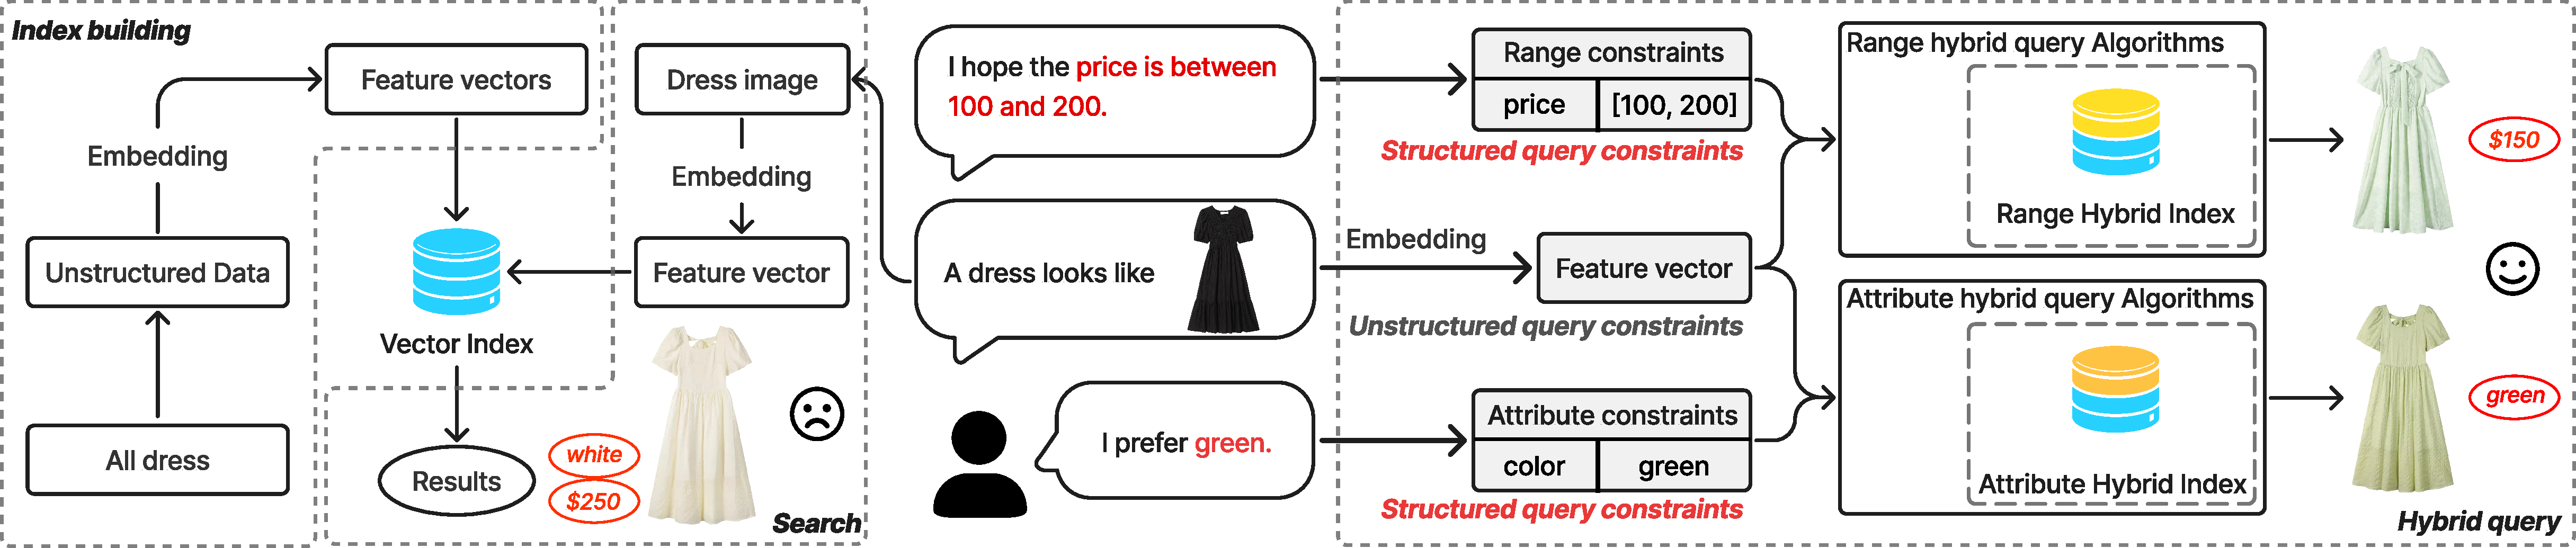
\includegraphics[width=0.92\textwidth]{figures/hybrid ANNS.pdf}
		\caption{Hybrid Query Example}
		
		\label{fig:hybrid ANNS}
	\end{figure*}
	\subsection{Motivation}
	
	In recent years, hybrid query algorithms develop rapidly, giving rise to numerous attribute filtering ~\cite{NHQ,diskann} and range filtering algorithms \cite{serf,iRangeGraph}. In practical applications, the performance of hybrid query algorithms is influenced not only by unstructured data but also closely related to structured data. For attribute filtering algorithms, factors such as the number of attributes, attribute distribution \cite{UNG}, and attribute  selectivity \textcolor{orange}{\cite{analyticdb,milvus}} significantly impact algorithm performance. As for range filtering algorithms, the size of the query range and the characteristics of different datasets  play an important role in determining algorithm performance.
	
	Despite BigANN 2023 \cite{bigann2023} evaluates the performance of some ANN algorithms, it presents several notable limitations:
	1) The evaluation covers a limited number of algorithms and fails to comprehensively include mainstream methods. 
	%	\sout{For instance, attribute filtering algorithms such as NHQ and UNG are not included in the evaluation. }
	2) It focuses only on single-attribute and dual-attribute query scenarios. 
	%	\sout{neglecting the more complex demands of multi-attribute queries. In real-world applications, an object typically involves multiple attributes.}\textcolor{blue}{ \sout{For example, in e-commerce scenarios, users often specify multiple attributes (e.g., color, brand, price range) simultaneously when searching.}}
	3) It does not evaluate algorithm performance under different attribute distributions. 
	%	\sout{However, variations in attribute distribution may directly affect the filtering strategies and index construction efficiency of hybrid query algorithms.}
	
%	Moreover, beyond BigANN, systematic evaluations of hybrid query algorithms remain limited.
%	To fill this gap, we conduct a comprehensive experimental evaluation of hybrid query algorithms, analyzing the index construction costs and query efficiency across different scenarios. Additionally, we further assess the robustness of each algorithm under varying conditions.
	
	Moreover, beyond BigANN, systematic evaluations of hybrid query algorithms remain limited. 
	\textcolor{orange}{%Although existing works \cite{compare,azizi2025graph} conduct benchmark evaluations or experimental analyses of ANN methods, existing work still lacks an experimental study specifically targeting hybrid query algorithms. 
	Although existing works\cite{compare,azizi2025graph} conduct benchmark evaluations of ANN methods, a dedicated experimental study on hybrid query algorithms is still lacking.
	To address this gap, we carry out the first comprehensive experimental evaluation of hybrid query algorithms, systematically analyzing their index construction costs and query efficiency across diverse scenarios. Furthermore, we rigorously assess the robustness of each algorithm under different experimental settings, thereby providing valuable insights for future research and practical applications.}
	
	\subsection{Our Contributions}
	
	Our study focuses on the problem of ANN search in hybrid query scenarios and provides a comprehensive review and evaluation of existing algorithms and systems. The main contributions are summarized in the following 5 aspects.
	
	(1)\textbf{ Systematic Classification and Overview.}
	We systematically classify 6 representative attribute filtering algorithms along multiple dimensions, including index organization, filtering strategies, Boolean logic support, and index construction methods. In addition, we survey 5 range filtering algorithms, and provide an overview of a vector library and three vector databases. These efforts offer a unified reference framework for future research.
%	\textcolor{orange}{%We systematically describe the distinct characteristics of 6 representative attribute filtering algorithms and 5 range filtering algorithms from various perspectives. We also provide an overview of these algorithms, along with a representative vector retrieval library and 3 vector databases, to help readers intuitively understand their design principles. This work offers a unified reference framework and technical foundation for future research in this field.}
%	We provide an overview of 6 representative attribute filtering algorithms and 5 range filtering algorithms from various perspectives, alongside a representative retrieval library and 3 vector databases. This work offers a unified reference framework and technical foundation for future research in this field.}
	
	(2) \textbf{Enhancing Datasets and Experimental Settings for Fair Evaluation.}
%		To ensure fair and reproducible evaluation, we generate attribute values based on real-world scenarios to enhance commonly used datasets. In addition to commonly used datasets, we also conduct experiments on a real-attribute dataset and a large-scale dataset (up to 100M records). Our benchmark design covers diverse selectivity levels and query conditions, establishing a unified and practical evaluation framework for hybrid query algorithms.}
%	To address the lack of standardized benchmarks in attribute filtering research, we generate attribute values based on real-world scenarios to enhance commonly used datasets. We also collect real attribute information from existing datasets and conduct experiments on a real attribute dataset to validate the plausibility of the generated attributes and the effectiveness of the results. To comprehensively reflect diverse real-world application needs, we design experiments covering varying attribute distributions, selectivity levels, and query conditions, ensuring representative and practical evaluation. \textcolor{cyan}{Furthermore, we test on a large-scale dataset containing 100 million records and a multi-modal dataset to analyze the scalability and performance of various algorithms.} These enhancements establish a unified evaluation framework that supports fair, consistent, and reproducible comparisons across different algorithms, laying a solid foundation for future research in hybrid query.
	To address the lack of standardized benchmarks in attribute filtering research, we enrich commonly used datasets by generating attribute values tailored to real-world scenarios. We design comprehensive experimental settings that reflect diverse application requirements, including varying attribute distributions, selectivity, and query conditions. \textcolor{cyan}{Furthermore, to investigate the scalability and adaptability of the algorithms, we conduct extended experiments on a large 100M dataset and a multi-modal dataset.} These enhancements provide a unified evaluation framework that supports fair, consistent, and reproducible comparisons across different algorithms, laying a solid foundation for future research in hybrid query.


%		To address the lack of standardized benchmarks in attribute filtering research, we enrich commonly used datasets by generating attribute values tailored to real-world scenarios. Furthermore, we design comprehensive experimental settings that reflect diverse application requirements, including varying attribute distributions, selectivity, and query conditions. These enhancements provide a unified evaluation framework that supports fair, consistent, and reproducible comparisons across different algorithms, laying a solid foundation for future research in hybrid query.

%	(3){ Evaluation of Attribute and Range Filtering Algorithms.}
%	\textcolor{cyan}{We conduct a comprehensive and integrated evaluation of 7 attribute filtering algorithms, 5 range filtering algorithms, 1 vector library, and 3 databases. We compare the index construction and query performance of each method across different scenarios using 5 core metrics. We identify the reasons for performance differences based on the design of the algorithms and summarize their respective strengths and weaknesses.}
	(3)\textbf{ Evaluation of Attribute Filtering Algorithms.}
	%We conduct a systematic evaluation of 13 attribute filtering algorithms on 7 real-world datasets. 
	We systematically evaluate 6 attribute filtering algorithms, 1 library, and 3 databases on 7 real-world datasets. By analyzing performance under varying numbers of attributes, we reveal the strengths and weaknesses of each method. We further examine their behavior under different attribute selectivity to assess robustness and adaptability in complex query scenarios. Evaluation metrics include index construction time, index size, peak memory usage, QPS, and search accuracy.
%	\textcolor{orange}{We conduct a comprehensive evaluation of 6 attribute filtering algorithms, 1 library, and 3 databases across 6 basic datasets, 2 real-world datasets, one 100M-scale dataset, and 2 multimodal datasets. By analyzing the query performance of each method under various scenarios, we reveal their respective strengths and weaknesses. We further examine their robustness by evaluating performance under different attribute distributions and selectivity levels. To ensure fairness and generality, we evaluate the methods on two different server environments. The evaluation metrics include index construction time, index size, peak memory usage, QPS, and search accuracy.}
%	

	(4)\textbf{ Evaluation of Range Filtering Algorithms.}
	We benchmark algorithms that support range filtering on 3 large-scale datasets, using varying query range settings in the experiments. The experimental results show the performance of these algorithms in terms of index construction efficiency, storage overhead, and query performance. We further analyze the factors that affect the performance of the range query algorithm.
%	\textcolor{orange}{
%		We conduct benchmark evaluations of range filtering algorithms on one synthetic and 2 real-world datasets, using various query range settings. Our experiments reveal and analyze the differences in time and query efficiency across these algorithms. Furthermore, we compare their performance on multimodal and large-scale datasets, and assess their adaptability across different server environments.
%	}
	
%	\textcolor{cyan}{{(4)\textbf{ Recommendations and Challenges.}
%	Based on the experimental results, we summarize a recommendation table in Section 5.1, which intuitively shows the suitable scenarios for each algorithm, allowing readers to select appropriate algorithms according to their own needs. In addition, we point out the challenges and the directions for future research in the field of hybrid querying.}}
	
	{(5)\textbf{ Recommendations and Challenges.}
%	Based on the experimental results, we provide a recommendation table that shows the performance of each algorithm in different scenarios. Readers can select suitable algorithms according to their specific application needs. In addition, we identify key challenges in the field of hybrid queries. These challenges include the lack of consideration for the correlation between attributes and vectors, limited support for Boolean logic, insufficient capability for multi-attribute range filtering, and sensitivity of algorithms to data distribution. Currently, few methods support both attribute filtering and range filtering at the same time. This indicates potential directions for future research.
%%}
	Based on the experimental results, we provide algorithm selection recommendations for common application scenarios and highlight key challenges in the field of hybrid queries. These challenges include limited Boolean logic support, the lack of multi-attribute range filtering capabilities, and the sensitivity of algorithms to data distribution. Currently, few methods simultaneously support both attribute filtering and range filtering, pointing to potential directions for future research.
	
	\section{PRELIMINARIES}
	
	\subsection{Problem Definition}
	
	We first define the Nearest Neighbor (NN) search problem.
	
	\begin{definition}[NN Search]
		
		Let \( D = \{v_1, \ldots, v_n\} \) be a dataset of \( n \) \( d \)-dimensional vectors. Given a query \( Q = (q_v, k) \), where \( q_v \) is the query vector and \( k \) is a positive integer, the NN search aims to return a set \( R \subseteq D \) with \( |R| = k \), such that for any \( x \in R \) and \( y \in D \setminus R \), \( \textit{dist}\!\left(q_v, x\right) \leq \textit{dist}\!\left(q_v, y\right) \). Here, \( \textit{dist}\!\left(\cdot, \cdot\right) \) denotes the distance metric, and we adopt Euclidean distance in this paper.
	\end{definition}
	
	However, to address the curse of dimensionality faced by NN search \cite{dimcurse}, existing studies focus on approximate solutions, known as ANN  search. We typically use $\text{Recall}@k = \frac{|R \cap \hat{R}|}{k}$ to evaluate the accuracy of ANN search algorithms, where $R$ denotes the true top-$k$ nearest neighbors of the query, and $\hat{R}$ denotes the approximate top-$k$ nearest neighbors returned by the ANN search algorithm.
	
	As the complexity of real-world application requirements increases, NN search has evolved into hybrid NN search with attribute constraints. Depending on the nature of the attribute constraints, hybrid NN search can be divided into 2 categories: 1) Attribute Filtering Nearest Neighbor (\textit{AF-NN}) search. 2) Range Filtering Nearest Neighbor (\textit{RF-NN}) search. We provide their formal definitions below.
	
	\begin{definition}[AF-NN Search]
		Let \( D = \{(v_1, s_1), \ldots, (v_n, s_n)\} \) be a dataset of \( n \) \( d \)-dimensional vectors, each associated with an attribute set \( s_i \). Given a query \( Q = (q_v, q_s, k) \), where \( q_s \) is the query attribute set, the AF-NN search aims to return a set \( R \subseteq D_s \) with \( |R| = k \), such that for any \( x \in R \) and \( y \in D_s \setminus R \), \( \textit{dist}(q_v, x) \leq \textit{dist}(q_v, y) \), where \( D_s = \{ v_i \mid (v_i, s_i) \in D \land q_s \subseteq s_i \} \).
	\end{definition}
	
	%	We further classify AF-NN search according to the number of the attribute set \( s_i \): 1) Single-Attribute Filtering Nearest Neighbor (\textit{SAF-NN}) search, where $\forall i,\, |s_i| = 1$. 2) Multi-Attribute Filtering Nearest Neighbor (\textit{MAF-NN}) search, where $\exists i,\, |s_i| > 1$.
	
	\begin{definition}[RF-NN Search]
		
		Let \( D = \{(v_1, \textcolor{cyan}{a}_1), \ldots, (v_n, \textcolor{cyan}{a}_n)\} \) be a dataset of \( n \) \( d \)-dimensional vectors, each associated with an attribute value \( a_i \). Given a query \( Q = (q_v, [a_{\min}, a_{\max}], k) \), where \( a_{\min} \) and \( a_{\max} \) denote the lower and upper bounds of the query range, respectively, the RF-NN search aims to return a set \( R \subseteq D_a \) with \( |R| = k \), such that for any \( x \in R \) and \( y \in D_a \setminus R \), \( \textit{dist}(q_v, x) \leq \textit{dist}(q_v, y) \), where \( D_a = \{ v_i \mid (v_i, a_i) \in D \land a_{\min} \leq a_i \leq a_{\max} \} \).
	\end{definition}
	
	
	
	Similar to the conventional ANN search, most existing studies focus on approximate solutions for hybrid NN search, referred to as hybrid ANN search, which includes both \textit{AF-ANN} search and \textit{RF-ANN} search.
	
	
	
%	\subsection{Index Organization in Hybrid ANN Search}
	\subsection{Index Organization}
	
	Current hybrid query methods mainly adopt graph-based ~\cite{nsw,kgraph,nsg,fanng,ngt} or Inverted File Index (IVF)-based \cite{PQ} index organization. 
	%We briefly introduce the fundamental principles of these two types in the following.
	\textcolor{violet}{Here, we briefly review the core concepts of these indexes and outline how attributes and range constraints are embedded to support hybrid query functionality.}
	
	\noindent\textbf{\underline{Graph.}}
	\textcolor{violet}{Graph structures accelerate ANN search by connecting each data point with its nearest neighbors, as shown in Figure~\ref{fig:graph}. During querying, algorithms start from an initial point and use a greedy strategy to progressively move towards closer neighbors until convergence (e.g., the path from $c$ to $j$ in the 1NN case).}
	
	\textcolor{violet}{Graph indexes are widely used in Hybrid ANN due to their efficiency. To support hybrid queries, in attribute filtering, a common practice involves attaching attribute metadata to nodes or edges, thereby skipping parts that do not satisfy query conditions during traversal (e.g., NHQ, Filtered-DiskANN, ACORN). In range filtering, edges typically store valid attribute intervals, and traversal proceeds only along edges that satisfy range constraints, thus narrowing the search space (e.g., SeRF, DSG).}
	
%	Graph-based ANN search algorithms accelerate queries by building graph indexes on datasets. As illustrated in Figure~\ref{fig:graph}, each data point in the dataset corresponds to a point in the graph, and neighboring vertices (e.g., $a$ and $b$) are connected via edges based on their distance $\textit{dist}(a, b)$. In the graph index, each point maintains connections only to its nearest neighbors to preserve query efficiency. For instance, in Figure~\ref{fig:graph}, the gray point $c$ is connected to 5 neighbors $(a, b, d, e, f)$ and can traverse to them via corresponding edges.
%	
%	Given a query point $q$, the graph-based ANN search typically follows a greedy search strategy to find the $k$ nearest neighbors. For illustration, consider the case where $k = 1$ (i.e., 1NN): The algorithm initiates the search from an entry point (the gray point $c$). If there exists a neighbor $n$ (the point $f$) of the current point such that $\textit{dist}(n, q) < \textit{dist}(c, q)$, the algorithm updates the current point to $n$. This process is iteratively repeated—always moving to the neighbor closest to $q$—until no neighbor is found that is closer than the current point. The final point reached (the blue point $j$) is returned as the approximate nearest neighbor of $q$.
%	
%	\textcolor{violet}{Graph-based indexes are widely adopted in Hybrid ANN search algorithms due to their excellent performance. To support hybrid queries, existing approaches usually augment the original graph structures by explicitly associating attribute or range information with vertices or edges. In attribute filtering, a common approach is to attach attribute metadata to vertices or edges, allowing the traversal process to skip nodes or edges that do not meet attribute conditions of the query (e.g., NHQ, Filtered-DiskANN, ACORN). In range filtering, edges typically store valid attribute intervals, and traversal proceeds only along edges satisfying the range constraints, effectively narrowing down the search space (e.g., SeRF, DSG).}
	
	
	\noindent\textbf{\underline{IVF.}} 
	\textcolor{violet}{IVF divides data into multiple clusters through clustering (e.g., K-Means), with each cluster represented by a center (Figure~\ref{fig:ivf}). During querying, algorithms search only within the few clusters closest to the query point, which reduces computational load.}
	
	\textcolor{violet}{IVF-based indexes also offer unique advantages in Hybrid ANN search scenarios, including natural support for pre-filtering, low memory footprint, and small index size. Efficient filtering is achieved by excluding vectors that do not satisfy attribute constraints before distance computation (e.g., Faiss, Milvus). Furthermore, hierarchical partitioning by attributes can form finer-grained sub-clusters to enhance filtering efficiency (e.g., CAPS, PUCK).}
%	IVF-based ANN search algorithms improve computational efficiency by partitioning the dataset into clusters and restricting the search to clusters nearest to the query point. Specifically, as shown in Figure~\ref{fig:ivf}, IVF first selects a subset of data points and applies a clustering algorithm (e.g., K-Means) to obtain a set of centroids $(C_0, C_1, ..., C_6)$, each representing a distinct cluster. Every data point (gray dots) is then assigned to the cluster corresponding to its nearest centroid based on the distance metric, thereby forming the index structure.
%	
%	During the query process, given a query point $q$, the algorithm computes distances between $q$ and all centroids, selects a small number of the closest centroids ($C_0, C_1, C_2$), and then performs a search only within the associated clusters to identify the approximate nearest neighbors.
%	
%	\textcolor{violet}{IVF-based indexes also offer unique advantages in Hybrid ANN search scenarios, such as naturally supporting pre-filtering and requiring significantly lower memory consumption and smaller index sizes compared to graph-based indexes. With minor modifications, IVF indexes achieve attribute and range filtering by directly excluding vectors that do not meet query constraints through pre-filtering, thus skipping irrelevant vectors during intra-cluster distance computations (e.g., Faiss, Milvus). Moreover, clusters can be further partitioned hierarchically based on attributes (hierarchical partitioning), resulting in finer-grained sub-partitions that significantly enhance the efficiency of attribute filtering (e.g., CAPS, PUCK).}
	
	\begin{figure}
		\begin{subfigure}{0.60\columnwidth}
			\centering
			
			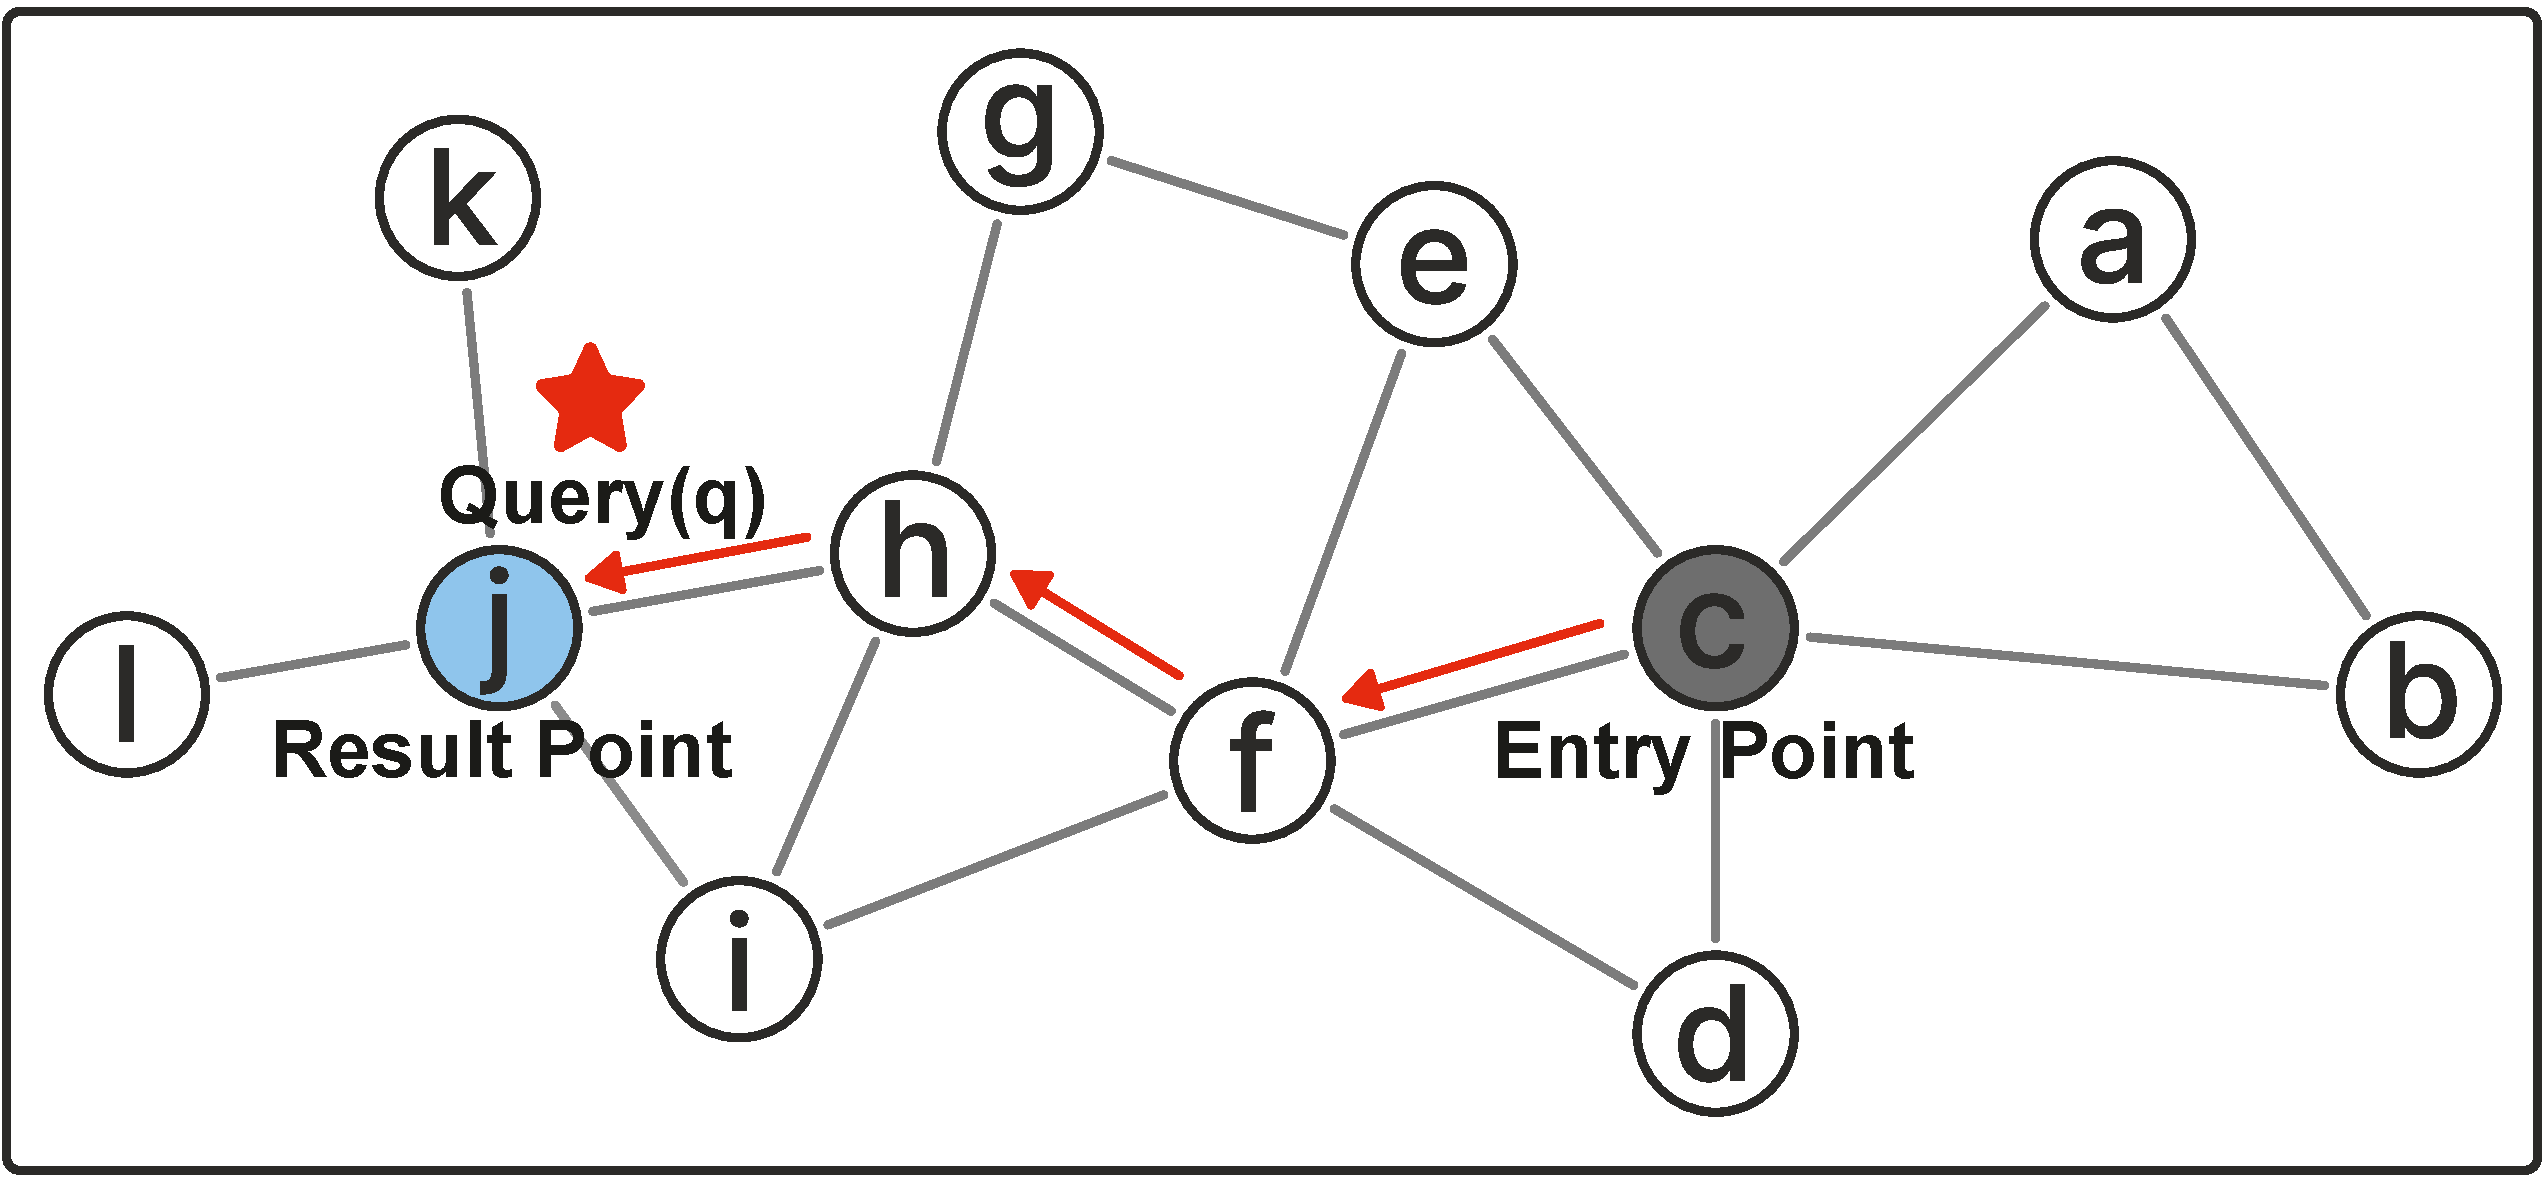
\includegraphics[width=\linewidth]{figures/graph.pdf}
			\caption{Graph Index}
			\label{fig:graph}
		\end{subfigure}
		\hfill
		\begin{subfigure}{0.38\columnwidth}
			\centering
			
			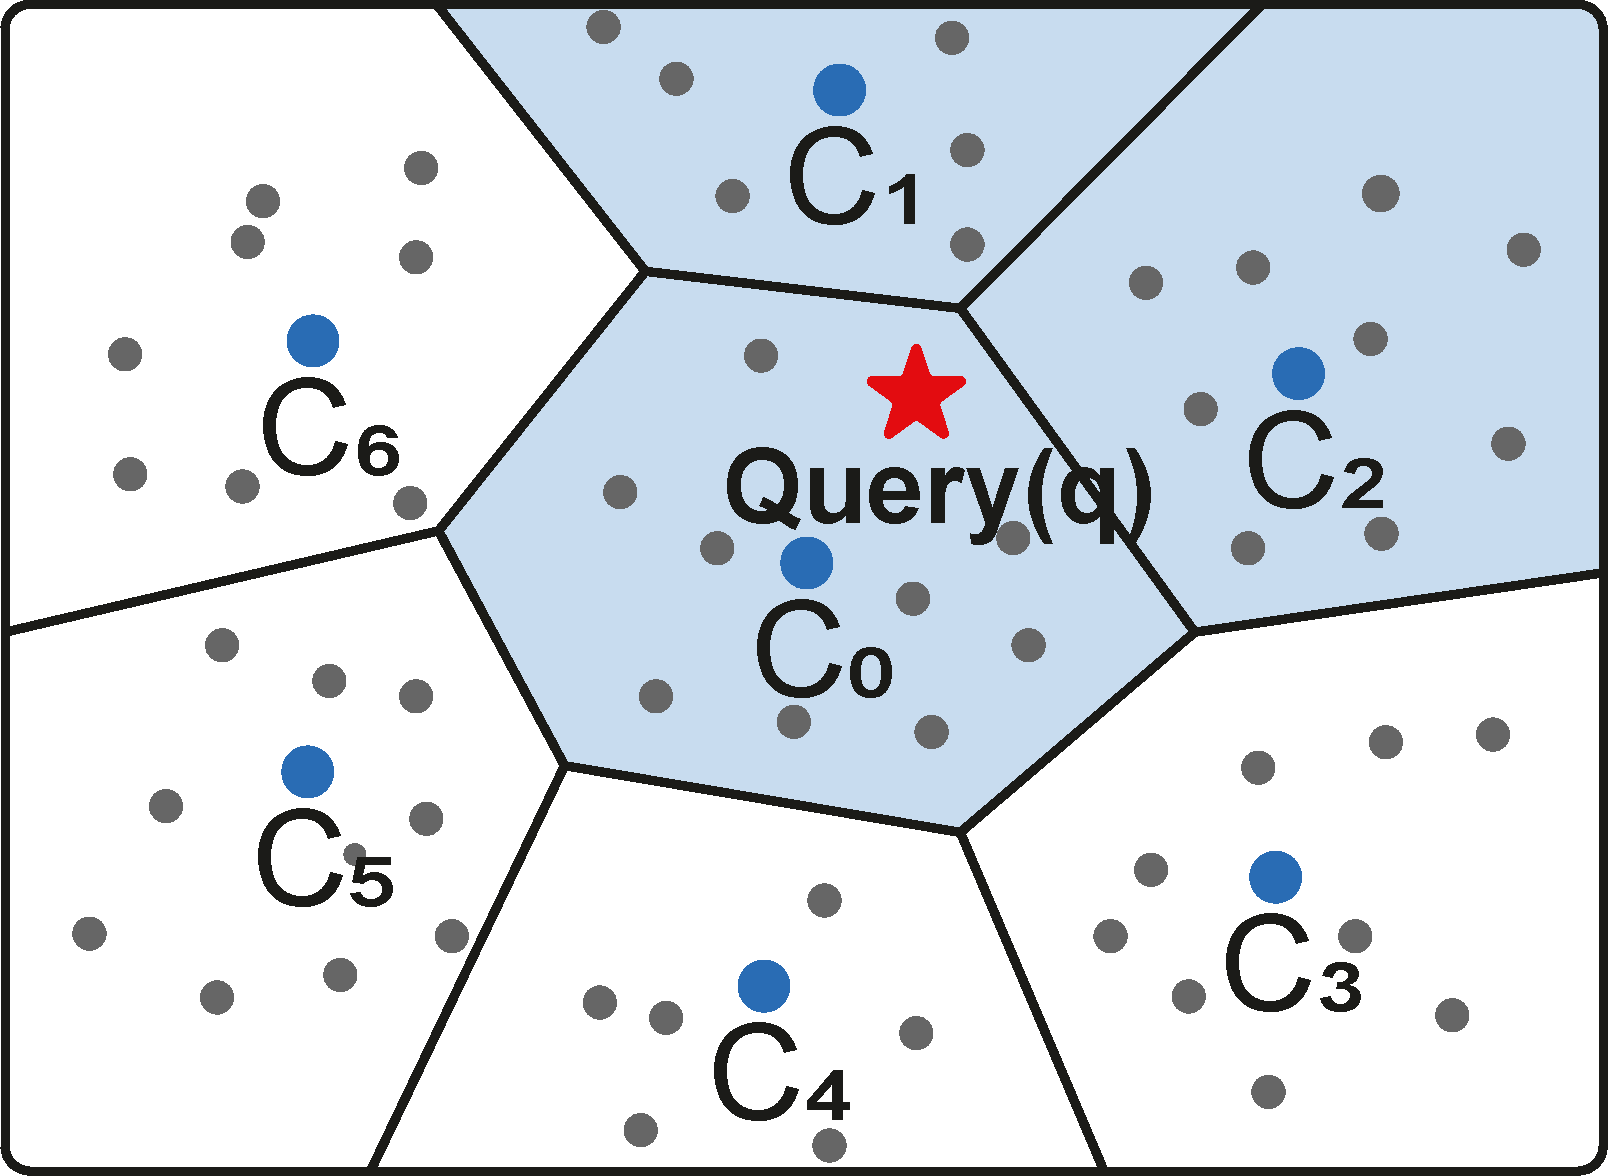
\includegraphics[width=\linewidth]{figures/ivf.pdf}
			\caption{IVF Index}
			\label{fig:ivf}
		\end{subfigure}
		
		
		\caption{Graph Index and IVF Index}
		
	\end{figure}
	
	
	\section{Hybrid query Algorithms}
	
	
	\renewcommand{\arraystretch}{0.9}
	\begin{table*}[t]
		\centering
		%\setlength{\belowcaptionskip}{-0.3cm}
		
		\caption{\textcolor{orange}{Comparison of AF-ANN and RF-ANN Search Algorithms}}
		\small
%		\label{tab:compair_1}
%		\begin{tabular}{|l|l|c|c|c|c|c|c|c|}
%			\hline
%			\textbf{Algorithm} & \textbf{Base} & \textbf{Filter Type} & \textbf{AND} & \textbf{OR} & \textbf{Flexible Attributes} & \textbf{Complex Boolean} & \textbf{Dynamic Insert} & \textbf{Multi Thread} \\
%			\hline
%			NHQ & Graph & C & Y & N& N& N & N & N \\
%			FilteredVamana & Graph & C & N & Y & Y & N & Y & Y \\
%			StitchedVamana & Graph & C & N & Y & Y & N & N & Y  \\
%			CAPS & IVF & C & Y & N & Y & N & Y & Y \\
%			ACORN & Graph & B & Y & Y & Y & Y & Y & Y \\
%			UNG & Graph & B & Y & Y & Y & N & Y & Y \\ 
%			Puck & IVF & B & Y & Y & Y & N & Y & Y \\
%			% ParlayANN & Graph+IVF & B & N & N & Y & N & N & Y \\
%			
%			\hline
%			
%		\end{tabular}
	\label{tab:compair_1}
	\begin{tabular}{|l|l|*{12}{c|}}
		\hline
		
	
		\multicolumn{2}{|c|}{\textbf{Characteristics/Algorithms}} & \textbf{NHQ} & \textbf{Filtered} & \textbf{Stitched} & \textbf{CAPS} & \textbf{ACORN} & \textbf{UNG} & \textbf{Puck} & \textbf{DSG} & \textbf{iRange} & \textbf{SeRF} & \textbf{UNIFY} & \textbf{Win}
		 \\ \hline
		\multirow{6}{*}{\textbf{AF}} 
		%& Filter Type         & C   & C   & C   & C   & B   & B   & B   & \multicolumn{5}{c|}{} \\ \cline{2-9}
		& AND                 & Y   & N   & N   & Y   & Y   & Y   & Y   & \multicolumn{5}{c|}{\multirow{4}{*}{\centering\shortstack{AF\\Not Support}}} \\ \cline{2-9}
		& OR                  & N   & Y   & Y   & N   & Y   & Y   & Y   & \multicolumn{5}{c|}{} \\ \cline{2-9}
		& Flexible Attributes & N   & Y   & Y   & Y   & Y   & Y   & Y   & \multicolumn{5}{c|}{} \\ \cline{2-9}
		& Complex Boolean     & N   & N   & N   & N   & Y   & N   & N   & \multicolumn{5}{c|}{} \\ \hline
		
		\multicolumn{2}{|l|}{\textbf{RF}}             & N & N & N & N & Y & N & N & Y & Y & Y & Y & Y \\ \hline
			\multicolumn{2}{|l|}{\textbf{Filter Type }}             & C & C & C & C & B & B & B & B & B & B & A/B/C & A \\ \hline
		\multicolumn{2}{|l|}{\textbf{Dynamic Insert}} & N & Y & N & Y & Y & Y & Y & N & Y & Y & Y & Y \\ \hline
		\multicolumn{2}{|l|}{\textbf{Multi Thread}}   & N & Y & Y & Y & Y & Y & Y & N & Y & Y & Y & Y \\ \hline
		\multicolumn{2}{|l|}{\textbf{Disk Support}}           &N  & Y& N & N & N & N & N & N & N & N & N & N \\ \hline
		\multicolumn{2}{|l|}{\textbf{Base}}           & Graph & Graph & Graph & IVF & Graph & Graph & IVF & Graph & Graph & Graph & Graph & Graph \\ \hline
	\end{tabular}
		
%		\begin{tabular}{|c|c|c|c|}
%			\hline
%			\textbf{Algorithm} & \textbf{Base} & \textbf{Dynamic Insert} & \textbf{Multi Thread} \\
%			\hline
%			DSG & Graph & Y & N \\
%			iRange & Graph & N & Y \\
%			SeRF & Graph & Y & Y \\
%			UNIFY & Graph & Y & Y \\
%			WinFilter & Graph & N & Y  \\
%			\hline
%		\end{tabular}
%		
		
		
		\centering
		%	 \setlength{\abovecaptionskip}{0cm}
		%	\setlength{\belowcaptionskip}{0.1cm}
		\footnotesize{
			\begin{minipage}{\linewidth}
				\vspace{0.1cm}
%				\textit{AND} and \textit{OR} indicate whether the algorithm supports the corresponding logical operations.
%				\textit{Flexible Attributes} indicates whether the number of query attributes can differ from the number of attributes used during index construction. 
%				\textit{Complex Boolean} indicates if the algorithm supports complex expressions, such as using the NOT operator or nested logic with parentheses.
%				\textit{Dynamic Insert} indicates whether the algorithm supports the operation of dynamically inserting data points.
%				\textit{Multi Thread} indicates whether the algorithm supports multi-threaded search.
%				\textit{Disk Support} indicates whether the algorithm supports disk storage.
%				\textit{Base} indicates the foundational ANN algorithm for the hybrid query method.
		\textcolor{orange}{
		\textit{Win}: WinFilter, \textit{Filtered}: FilteredVamana, \textit{Stitched}: StitchedVamana. 
		\textit{AND} / \textit{OR}: Whether the algorithm supports the corresponding logical operations.
		\textit{Flexible Attributes}: Allows the number of query attributes to differ from that in index construction.
		\textit{Complex Boolean}: Supports NOT or nested Boolean expressions.
		\textit{Dynamic Insert}: Supports dynamic data insertion.
		\textit{Multi Thread}: Supports multi-threaded search.
		\textit{Disk Support}: Supports disk-based storage.
		\textit{Base}: Underlying ANN index structure used.}
		\textsuperscript{A} Post-filtering, 
		\textsuperscript{B} Pre-filtering, 
		\textsuperscript{C} Simultaneous filtering, 
		\textsuperscript{Y} Support, 
		\textsuperscript{N} Unsupport. 
		\end{minipage}}
		
	\end{table*}
	
	
	%We provide an overview and analysis of 15 hybrid query methods, all drawn from recent studies, and collectively referred to as algorithms in the following. Specifically, Section~3.1 describes methods for attribute filtering, Section~3.2 discusses those for range filtering, and Section~3.3 introduces vector libraries and databases that support both attribute filtering and range filtering.
	Table~\ref{tab:compair_1} provides a comparative overview of six attribute filtering and five representative range filtering algorithms. 
	
	\subsection{Attribute Filtering Algorithms}
	

%	\noindent\textbf{\underline{NHQ \cite{NHQ}.}}  
%	\footnote{https://github.com/KGLab-HDU/TKDE-under-review-Native-Hybrid-Queries-via-ANNS}
	\noindent\textbf{\underline{NHQ} \footnote{\textcolor{blue}{https://github.com/KGLab-HDU/TKDE-under-review-Native-Hybrid-Queries-via-ANNS}} \cite{NHQ}}
	Traditional attribute filtering algorithms usually perform attribute constraints and ANN search separately. In contrast, NHQ is the first to implement simultaneous filtering, integrating both aspects into a unified framework. NHQ constructs an index based on a nearest neighbor graph and introduces a fusion distance that jointly captures vector similarity and attribute similarity. Leveraging this fusion distance, NHQ unifies vector similarity and attribute matching into a single comprehensive similarity measure and builds the graph accordingly. During the query process, NHQ efficiently prunes irrelevant edges via this composite index, enabling fast retrieval of results that satisfy both vector similarity and attribute constraints.
	
	\noindent\textbf{\underline{Filtered-DiskANN} \footnote{\textcolor{blue}{https://github.com/microsoft/DiskANN}} \cite{Filtered-diskann}}
	%\sout{The effectiveness of NHQ may degrade when the number of attributes changes, as it affects the fusion distance computation. Filtered-DiskANN addresses this limitation.}
	Filtered-DiskANN also supports simultaneous filtering. Built upon the Vamana \cite{diskann} graph-based ANN index, it incorporates attribute information directly into the graph during index construction. This integration ensures that the index reflects both vector similarity and attribute constraints. Moreover, Filtered-DiskANN supports SSD-based storage, improving scalability.
	Filtered-DiskANN proposes 2 indexes:  
	1) \textbf{FilteredVamana}, which incrementally builds the graph index by inserting data points and dynamically adding edges, allowing adaptive expansion.  
	2) \textbf{StitchedVamana}, which adopts a batch construction strategy—constructing separate Vamana subgraphs for each attribute, followed by merging and edge pruning.
	%	A key limitation of Filtered-DiskANN is that only supports the Boolean OR logic for multi-attribute filtering, lacking support for Boolean AND logic.
	
	
	\noindent\textbf{\underline{CAPS} \footnote{\textcolor{blue}{https://github.com/gaurav16gupta/constrainedANN}} \cite{CAPS}}
	%\sout{Different from the above graph-based simultaneous filtering algorithms,}
	CAPS is the first simultaneous filtering algorithm based on spatial partitioning.
	It introduces a hierarchical sub-partitioning algorithm inspired by Huffman trees, termed the Attribute Frequency Tree (AFT), to overcome the coarse granularity of traditional IVF-based methods. CAPS adopts a two-level partitioning strategy:  
	1) The first level clusters vectors based on similarity using K-Means or learning-based methods such as BLISS. 2) Within each cluster, AFT partitions data further based on attribute frequencies, enabling finer-grained indexing and improving query efficiency.
	
	\noindent\textbf{\underline{ACORN} \footnote{\textcolor{blue}{https://github.com/stanford-futuredata/ACORN}} \cite{ACORN}}
	%	Above simultaneous filtering algorithms struggle with large-scale, unbounded, or unknown predicate sets.
	%	%The above simultaneous filtering methods are less effective in scenarios involving large-scale, unbounded, or unknown predicate sets, where a predicate refers to a condition or rule used for filtering. 
	%	ACORN addresses this issue by introducing a predicate-agnostic indexing framework.
	%	ACORN is built upon Hierarchical Navigable Small World (HNSW) \cite{hnsw}. It supports high-cardinality and unrestricted predicate sets, overcoming the limitations of methods restricted to small-scale equality filters. It constructs a denser hierarchical graph by expanding node neighborhoods and prunes edges at lower levels to control index size. During the query process, ACORN eliminates unnecessary distance computations by filtering out nodes that violate attribute constraints. This effectively maintains a nearest neighbor graph over valid nodes only. 
	%	%During the query process, ACORN avoids unnecessary distance computations by filtering out nodes that do not meet attribute constraints, effectively simulating a nearest neighbor graph over valid nodes only.
	%	ACORN includes 2 indexes: 1) \textbf{ACORN-$\gamma$}, which expands neighbor lists during construction, increasing memory usage for higher performance.  
	%	2) \textbf{ACORN-1}, which extends neighbor lists by considering second-hop neighbors during search, reducing index size with minor performance loss.
	%Above simultaneous filtering algorithms struggle with large-scale, unbounded, or unknown predicate sets. ACORN addresses this by introducing a predicate-agnostic indexing framework.
	Pre-filtering methods apply attribute constraints prior to ANN search. As a pre-filtering approach, ACORN adopts a predicate-agnostic indexing framework to overcome the limitations of the aforementioned simultaneous filtering methods in handling large-scale or unknown predicate settings.
	Based on Hierarchical Navigable Small World (HNSW) \cite{hnsw}, ACORN constructs a denser hierarchical graph with neighborhood expansion and edge pruning. During search, it filters out nodes violating constraints, maintaining a valid nearest neighbor graph.
	ACORN includes two indexes: 1) \textbf{ACORN-$\gamma$}, which expands neighbor lists during construction, trading memory for higher performance; 
	2) \textbf{ACORN-1}, which extends neighbor lists via second-hop neighbors during search, reducing index size with minor performance loss.
	
	\noindent\textbf{\underline{UNG} \footnote{\textcolor{blue}{https://github.com/YZ-Cai/Unified-Navigating-Graph}} \cite{UNG}} 
	%\sout{The above simultaneous filtering algorithms may not guarantee the completeness of the results and perform poorly when the attribute selectivity is low. UNG is proposed to overcome these limitations.It is a unified framework that integrates diverse graph-based ANN indexes for hybrid query.}
	Similar to ACORN, UNG adopts a pre-filtering strategy and serves as a unified framework that integrates various graph-based ANN indexes to support hybrid queries. It first groups the dataset by attribute sets, ensuring that vectors in each group share identical attributes. Then, it constructs a Label Navigating Graph (LNG) to encode inclusion relationships among attribute sets. Within each group, UNG builds graph-based ANN indexes (e.g., Vamana, HNSW) and connects them via cross-group edges to enable efficient cross-group search.
	%UNG supports Boolean filtering with 2 modes:  1) The query attribute set is a subset of the data attribute set.  2) The query attribute set exactly matches the data attribute set.
	
	
	
	\noindent\textbf{\underline{Puck} \footnote{\textcolor{blue}{https://github.com/baidu/puck}} \cite{puck}} 
	%While simultaneous filtering algorithms perform well in most scenarios, it may underperform when only a small portion of data satisfies attribute constraints. In such cases, a pre-filtering strategy—applying attribute constraints prior to ANN search—can be more effective.
	Puck also adopts a pre-filtering strategy. Developed by Baidu, Puck utilizes two-level quantization for indexing. It maintains an attribute set for each cluster to track vector attributes. During the query process, it employs pre-filtering to exclude clusters without required attributes, thereby reducing the search space.
	%Developed by Baidu, Puck adopts a pre-filtering approach and employs a multi-level filtering mechanism for hybrid query. Its index structure comprises four layers: the first two use vector quantization for training, while the latter two leverage product quantization.
	
	
	
%	\renewcommand{\arraystretch}{0.9}
%	\begin{table}[t]
%		\centering
%		
%		\setlength{\textfloatsep}{0.1cm}
%		\caption{Comparison of RF-ANN search algorithms}
%		\small	% 只会影响当前组的内容
%		\label{tab:range_algo}
%		\begin{tabular}{|c|c|c|c|}
%			\hline
%			\textbf{Algorithm} & \textbf{Base} & \textbf{Dynamic Insert} & \textbf{Multi Thread} \\
%			\hline
%			DSG & Graph & Y & N \\
%			iRange & Graph & N & Y \\
%			SeRF & Graph & Y & Y \\
%			UNIFY & Graph & Y & Y \\
%			WinFilter & Graph & N & Y  \\
%			\hline
%		\end{tabular}
%		
%		
%		\footnotesize{
%			\begin{minipage}{\linewidth}
%				\centering
%				The indicators are consistent with those in Table ~\ref{tab:compair_1}.
%				%				\textsuperscript{Y} Support, 
%				%				\textsuperscript{N} Unsupport.
%				%				\textit{Base} indicates that the hybrid query algorithm is an improvement based on a specific ANN search algorithm. 
%				%				\textit{Dynamic Insert} indicates whether the algorithm supports the operation of dynamically inserting data points.
%				%				\textit{Multi Thread} indicates whether the algorithm supports multi-threaded search.
%			\end{minipage} 
%			
%		}
%		
%	\end{table}
	
	\subsection{Range Filtering Algorithms}
	
	\noindent\textbf{\underline{SeRF} \footnote{\textcolor{blue}{https://github.com/rutgers-db/SeRF}} \cite{serf}} Conventional RF-ANN search approaches typically follow one of two paradigms: 1) Conducting ANN search first followed by attribute-based filtering. 2) Filtering the dataset based on attribute ranges before performing ANN search. Building a separate neighbor graph (e.g., HNSW) for each attribute range could ensure efficient querying but incurs an $O(n^2)$ cost in constructing and storing $n$ graphs. Since many edges are shared across these graphs, SeRF introduces a validity-range aware design where each edge records the interval in which it is valid, indicating in which subgraphs the edge remains valid. This compresses $n$ graphs into a single unified graph, maintaining search effectiveness while significantly reducing memory and index construction overhead.
	
	\noindent\textbf{\underline{WinFilter} \footnote{\textcolor{blue}{https://github.com/JoshEngels/RangeFilteredANN}} \cite{winFilter}}
	Unlike SeRF, which focuses on graph compression, WinFilter proposes a structural partitioning framework called the $\beta$-Window Search Tree ($\beta$-WST). After the dataset is sorted by attribute values, it is partitioned into multiple intervals and organized into a tree structure. Each node in the tree corresponds to an attribute range and maintains a local ANN index (e.g., Vamana). For a range filtering query, WinFilter only searches within nodes overlapping the query range and merges partial results. With a tree height of $O(\log n)$, each query accesses at most $O(\log n)$ sub-indexes, resulting in significant speedups.
	
	\noindent\textbf{\underline{iRange} \footnote{\textcolor{blue}{https://github.com/YuexuanXu7/iRangeGraph}} \cite{iRangeGraph}}
	To address the query efficiency degradation caused by the graph compression in SeRF, iRange adopts a more flexible strategy.
	%Rather than prebuilding indexes for all possible ranges, it dynamically assembles a query-specific subgraph at runtime.
	iRange partitions the dataset into intervals based on attribute values and independently constructs a local graph for each interval, storing only edge information. During the query process, the relevant local graphs overlapping with the query range are merged into a temporary search graph, and a pruning strategy is applied to enable efficient search.
	
	\noindent\textbf{\underline{DSG} \footnote{\textcolor{blue}{https://github.com/rutgers-db/DynamicSegmentGraph}} \cite{DSG}}
	Most RF-ANN search methods, such as iRange and WinFilter, are designed for static datasets. SeRF allows incremental insertion but requires ordered attributes. DSG introduces the first dynamic RF-ANN framework supporting data insertion with unordered attributes while maintaining efficient range filtering.
	DSG relies on two data structures: 1) A rectangle tree partitions query space into rectangular regions, each corresponding to a group of queries sharing nearest neighbors. 2) A dynamic segment graph is a neighbor graph where each edge is annotated with its valid attribute range.
	With these structures, only few regions need updates when inserting new data. The system considers only edges valid for current attribute range to boost efficiency during search.
	
	\noindent\textbf{\underline{UNIFY} \footnote{\textcolor{blue}{https://github.com/sjtu-dbgroup/UNIFY}} \cite{UNIFY}}
	Unlike DSG, which relies on rectangle trees and range-aware edges, UNIFY adopts a segmentation-based approach and proposes a range query index structure. UNIFY introduces the Segmented Inclusive Graph (SIG), which partitions the dataset into segments by attribute and constructs an independent neighbor graph for each segment. These segment graphs are then integrated into a unified global graph. Its hierarchical variant, HSIG, enhances SIG by incorporating the multilayer design of HNSW, skip lists, and edge bitmaps for efficient range localization and post-filtering pruning. UNIFY supports 3 filtering strategies—pre-filtering, post-filtering, and  simultaneous filtering—enabling robust and flexible performance.
	
	
	
	\subsection{Vector Libraries and Databases}
	
	The vector libraries and databases discussed in the following are not explicitly designed for hybrid query, but they support both attribute filtering and range filtering. Additionally, all the functionalities shown in Table 1 are also supported.
	
	\noindent\textbf{\underline{Faiss} \footnote{\textcolor{blue}{https://github.com/facebookresearch/faiss}} \cite{Faiss}}
	Faiss is a library designed for efficient similarity search. It supports various indexing structures, including IVF, Product Quantization (PQ) \cite{PQ}, and HNSW. In hybrid query scenarios, Faiss supports vector search with an ID selector, which is a bitmap aligned with the dataset size. Users can generate this selector by first applying custom attribute filtering methods. During the query process, Faiss excludes vectors based on the selector, enabling efficient integration of attribute filtering with ANN search. In addition, we adopt the batch optimization strategy of HQI~\cite{HQI} for the IVF index in Faiss. This strategy groups queries with the same filter conditions, performs filtering once per group, and then uses efficient matrix operations to perform batch vector similarity calculations.
	
	
	\noindent\textbf{\underline{PASE} \footnote{\textcolor{blue}{https://github.com/alipay/PASE}} \cite{pase}}
	PASE is a vector indexing plugin for the PostgreSQL database \cite{postgresql13.4}, supporting two index types: IVF\_Flat \cite{johnson2019billion} and HNSW. By leveraging database capabilities, PASE enables both attribute filtering and range filtering. We focus on the post-filtering strategy based on HNSW, which facilitate comparison with other methods. When a query request is received, PASE first obtains a candidate set using the HNSW index. It then applies the filtering conditions from the WHERE clause to refine the results. However, since the candidate set has a fixed size, low-selectivity filters may result in fewer than $k$ results being returned.
	
	
	\noindent\textbf{\underline{VBASE} \footnote{\textcolor{blue}{https://github.com/microsoft/MSVBASE}} \cite{vbase}}
	Similar to PASE, VBASE is a PostgreSQL-based vector indexing plugin supporting HNSW, SPTAG~\cite{sptag}, and SPANN~\cite{spann}. We focus on HNSW-based search because SPTAG and SPANN have poorer performance and their source code does not fully implement index-building functionality. VBASE adopts a post-filtering strategy. However, it employs an iterative filtering mechanism: during index traversal, each node is checked against the WHERE clause, and non-matching nodes are discarded. This avoids the issue in PASE where the final result set may contain fewer than $k$ results.
	
	\noindent\textbf{\underline{Milvus} \footnote{\textcolor{blue}{https://github.com/milvus-io/milvus}} \cite{milvus}}
	Unlike PASE and VBASE, which are database extensions, Milvus is an vector database purpose-built for large-scale similarity search. It supports multiple index types, including HNSW, IVF\_Flat, and IVF\_PQ, and provides extensive optimization for real-world deployment. Among its indexes, IVF\_Flat is commonly used due to its balance between performance and simplicity. In hybrid queries, Milvus first pre-filters the dataset using user-specified conditions, then traverses only the corresponding clusters for ANN search—similar to the ID selector mechanism of Faiss.
	
	\section{Experiments}
	\subsection{Experimental Setup}
	\subsubsection{Datasets}
	
	\textcolor{violet}{Our experiments employ 12 real-world datasets covering diverse domains: Audio~\cite{audio_unknown}, Deep1M~\cite{yandex_deep_dataset}, Enron~\cite{enron2015}, GIST1M~\cite{sift2010}, GloVe~\cite{GloVe2015}, Msong~\cite{msong2011}, SIFT1M~\cite{sift2010}, WIT-Real~\cite{wit_dataset}, YT-Audio-Real~\cite{youtube8m_dataset}, Text2image~\cite{texttoimage}, Text2image-Mix, and Deep100M.}
	
	\textcolor{violet}{The first seven datasets are widely used in existing works. As they do not inherently come with attributes, we generate attributes for them to precisely control attribute quantity and distribution.}
	
	\textcolor{violet}{WIT-Real and YT-Audio-Real datasets use real attributes. For the WIT-Real dataset, we use the CLIP model to encode the page title into vectors, and extract the language type and the length of the context page description  as real attributes. The YT-Audio-Real dataset uses YouTube8M data, employing the video category ID and view counts as real attributes for this dataset.}
	
	\textcolor{violet}{Additionally, we use the Out-of-Distribution (OOD) dataset Text2Image and the large-scale dataset Deep100M to evaluate the generalization capability of the algorithms. The Text2Image dataset includes two versions. The original version contains 1 million image embeddings as the base dataset and uses 10 thousand text embeddings as the query set. The Text2Image-Mix version is composed of 0.5 million image embeddings and 0.5 million text embeddings as the base dataset, with a query set of 5 thousand image embeddings and 5 thousand text embeddings.}
	
	Table~\ref{tab:datasets_combined} summarizes the key characteristics of all datasets and their applicable filtering scenarios. In particular, we report the Local Intrinsic Dimensionality (LID)~\cite{Lid}, which is a commonly used metric to quantify dataset hardness. Following the standard evaluation protocol~\cite{LID2}, we randomly sample 10,000 data points from each dataset to compute LID. The higher the LID value, the harder the dataset.
	
	%For attribute filtering tasks, we employ 6 real-world datasets widely adopted in existing literature: Msong~\cite{msong2011}, Audio~\cite{audio_unknown}, SIFT1M~\cite{sift2010}, GIST1M~\cite{sift2010}, GloVe~\cite{GloVe2015}, Enron~\cite{enron2015}, covering a diverse range of domains. We independently generate attribute for each dataset.
	
	%\textcolor{violet}{For range filtering queries, we evaluate 1 widely used dataset: WIT~\cite{wit_dataset}. Following prior work~\cite{DSG}, we use the data point ID within each dataset as its attribute. This ensures that the data is initially sorted.}
	
	%\textcolor{violet}{Additionally, we introduced two datasets with real attributes for a more comprehensive evaluation of various attribute filtering and range query algorithms: The YT-Audio-Real dataset leverages URLs provided by the YouTube8M dataset to crawl corresponding video category IDs and view counts as its real attributes; whereas for the WIT-Real dataset, we used the \texttt{clip-vit-base-patch32} model to encode the \texttt{page\_title} field into vectors, and used the language type and the length of the \texttt{context\_page\_description} field as real attributes. It should be noted that, during range filtering, due to the limitations of some algorithms, we uniformly sorted the vectors according to the query attribute.}
	
	%\textcolor{violet}{To validate the algorithm generalization capability, we also further evaluated the performance of various algorithms on the Out-of-Distribution (OOD) dataset Text2Image~\cite{texttoimage} and the large-scale dataset Deep100M. Specifically, the Text2Image dataset comprises two versions: the original version contains 1 million image embeddings as the base dataset and uses 10 thousand text embeddings as the query set; the Text2Image-Mix version is composed of 0.5 million image embeddings and 0.5 million text embeddings as the base dataset, with a query set of 5 thousand image embeddings and 5 thousand text embeddings.}
	
%	In addition, we evaluate the performance of different algorithms on the Out-of-Distribution (OOD) dataset Text2Image~\cite{texttoimage}.		
	
	%Table~\ref{tab:datasets_combined} summarizes the key characteristics of all datasets. In particular, we report the Local Intrinsic Dimensionality (LID)~\cite{Lid}, a commonly used metric to quantify dataset hardness. Following the standard evaluation protocol~\cite{LID2}, we randomly sample 10,000 data points from each dataset for LID computation.The higher the LID value, the harder the dataset.
	
	
	\renewcommand{\arraystretch}{0.9}
	\begin{table}[t]
		\centering
		
		
		
		\caption{Datasets}
		
		\label{tab:datasets_combined}
		\resizebox{\columnwidth}{!}{
			\begin{tabular}{ccccccc}
				\toprule
				Dataset & Dimension & Base Data & Queries & LID & Type& Used \\
				\midrule
				
				Audio & 192 & 53,387 & 200 & 14& Audio& AF \\
				Enron & 1369 & 94,987 & 200 & 23& Text& AF \\
				GIST1M & 960 & 1,000,000 & 1,000 & 45& Image& AF \\
				GloVe & 100 & 1,183,514 & 10,000 & 47& Text& AF \\
				Msong & 420 & 992,272 & 200 & 23& Audio& AF \\
				SIFT1M & 128 & 1,000,000 & 10,000 & 19& Image& AF \\
				
				%YT-Audio& 128 & 1,000,000 & 10,000 & 15& Audio \\
				Deep1M & 96 & 1,000,000 & 10,000 & 22 & Image& RF \\
				YT-Audio-Real& 128 & 1,000,000 & 10,000 & 15& Audio& Both \\
				WIT-Real & 512 & 1,000,000 & 40,300 & 48& Image& Both \\
				Text2Image & 200 & 10,000,000 &10,000 & 59& Text,Image& Both \\
				Text2Image-Mix & 200 & 1,000,000 &10,000 & 59& Text,Image& Both \\
				Deep100M & 96 & 100,000,000 & 10,000 & 22& Image& Both \\
				\bottomrule
			\end{tabular}
		}
	\end{table}
	
	
	
	
	
	
	\subsubsection{Evaluation Metrics}
	
	To assess the overall performance of different algorithms, we adopt a multi-dimensional quantitative evaluation framework~\cite{compare}, including the following 5 core metrics:
	
	\begin{enumerate}
		
		\item \textbf{Recall@k}: The proportion of overlap between the returned approximate $k$ nearest neighbors and the ground-truth $k$ nearest neighbors.
		\item \textbf{QPS (Queries Per Second)}: The number of queries processed per second.
		\item \textbf{Index Construction Time}: The total time required to transform the raw dataset into a queryable index structure.
		\item \textbf{Index Size}: The storage size of the persisted index on disk.
		\item \textbf{Peak Memory Usage}: The maximum memory consumption observed during index construction \textcolor{cyan}{and search}.
	\end{enumerate}
	
	%\subsubsection{Parameter Settings}
	
	%\textcolor{blue}{For all algorithms, we adopt recommended settings from the original study and adjust the parameters related to search in order to obtain different Recall and QPS.}
	
	
	
	\subsubsection{\textcolor{cyan}{Setting}}
	
	
	We conduct most experiments on a server running Ubuntu 20.04, equipped with an AMD EPYC 7K62 processor (2.6GHz) featuring 256GB of RAM and 192 MiB of L3 cache.  
%	\textcolor{cyan}{Additionally, to investigate the impact of different server configurations on algorithm performance, we also conducted partial experiments on a server equipped with dual Intel(R) Xeon(R) Gold 6330 CPU @ 2.00GHz and 128GB of RAM. For clarity and conciseness, we hereafter refer to the former as Server A and the latter as Server B. Unless otherwise specified, all experiments were conducted on Server A.} 
	Unless otherwise stated, we execute index construction with 32 threads to accelerate the process~\cite{benchmarkindex}. By default, queries run on a single thread. We also report results for 16-thread parallelism in specific scenarios. We summarize the multi-threading capabilities of each algorithm in Table~\ref{tab:compair_1}. For vector database systems, we adopt a multi-process evaluation scheme (rather than multi-threaded execution), following the methodology proposed in VectorDBBench~\cite{VectorDBBench}, to better reflect their real-world performance.
	
	\textcolor{cyan}{
	Regarding experimental parameter selection, we adopted the recommended settings from original papers when available. For datasets without suggested parameters, we experimented with different configurations and selected the optimal one for final evaluation. Due to the extensive number of datasets and algorithms involved, specific parameters are not listed individually but are provided in our code repository.
}
%	\textcolor{blue}{
%	\subsubsection{Parameters}
%	In the experiments, for datasets with recommended parameters in the original paper, we use the recommended settings. For datasets without recommended parameters, we conduct experiments with different parameter settings and select the one that performs best for the final experiment. Due to the large number of datasets and algorithms involved, the parameters are not listed individually, but they are provided in the code repository.
%}
	
	
	%4.2
	\subsection{Attribute Filtering}
	
	
	%4.2.1
	\subsubsection{\textcolor{violet}{Time and Space overhead}}
	% \subsubsection{\textbf{Attribute Filtering}}
	\begin{figure}[t]
		\centering
		
		
		% 上面的图例,居中并可通过 hspace 调整左右位置
		\hspace*{8pt} % 可调整的参数,负值左移,正值右移,例如 -20pt 或 20pt
		
\includegraphics[width=0.95\columnwidth]{figures/indexData/legend_only.pdf} % 图例图片路径
		
		
		\begin{subfigure}{\columnwidth}
			\centering
			
			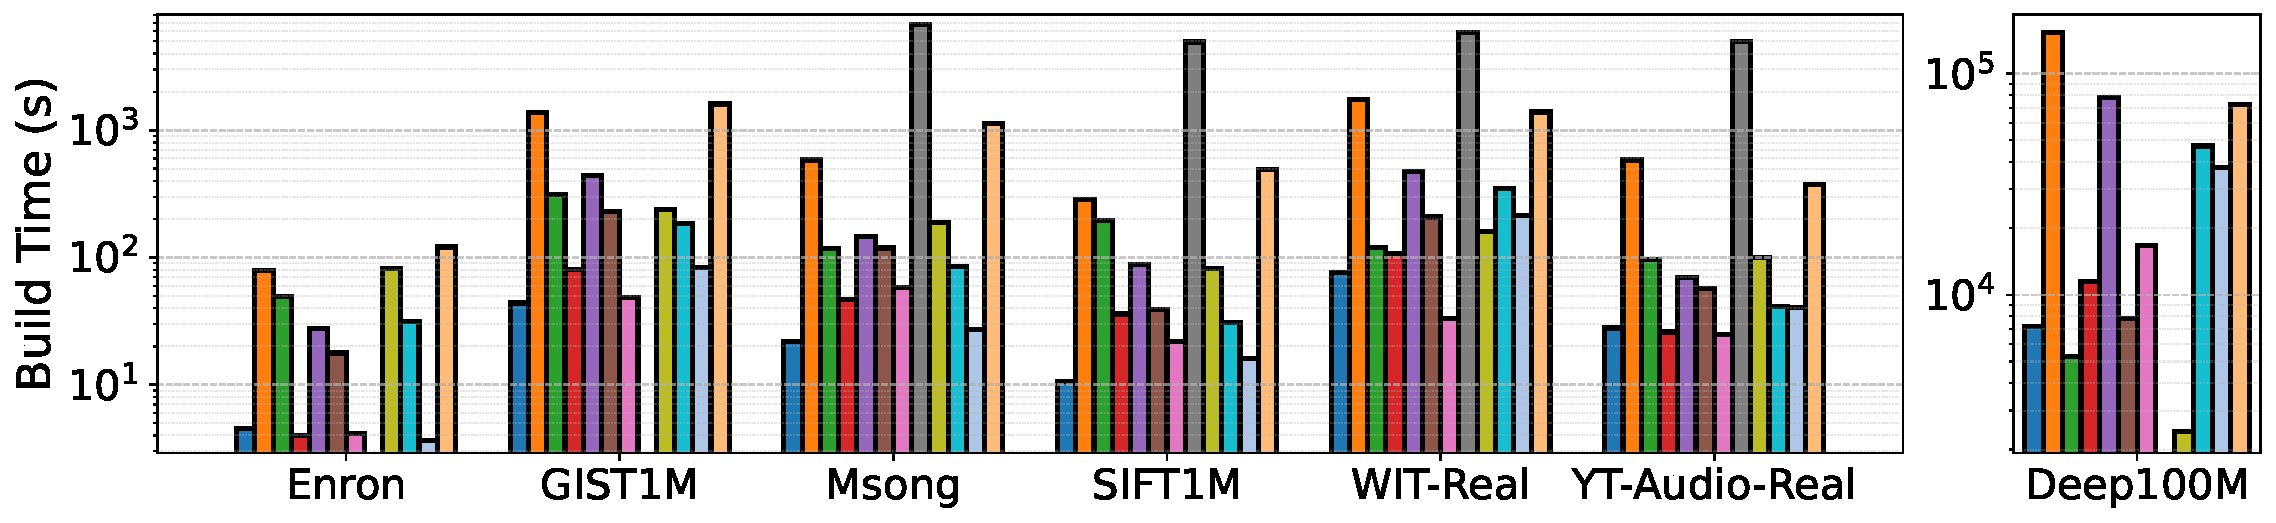
\includegraphics[width=0.99\linewidth]{figures/indexData/exp_7_build_time_comparison_query1.pdf}
			\caption{Construction Time}
			\label{fig:build_time_comparison_query1}
		\end{subfigure}
		
		
		
		\begin{subfigure}{\columnwidth}
			\centering
			
			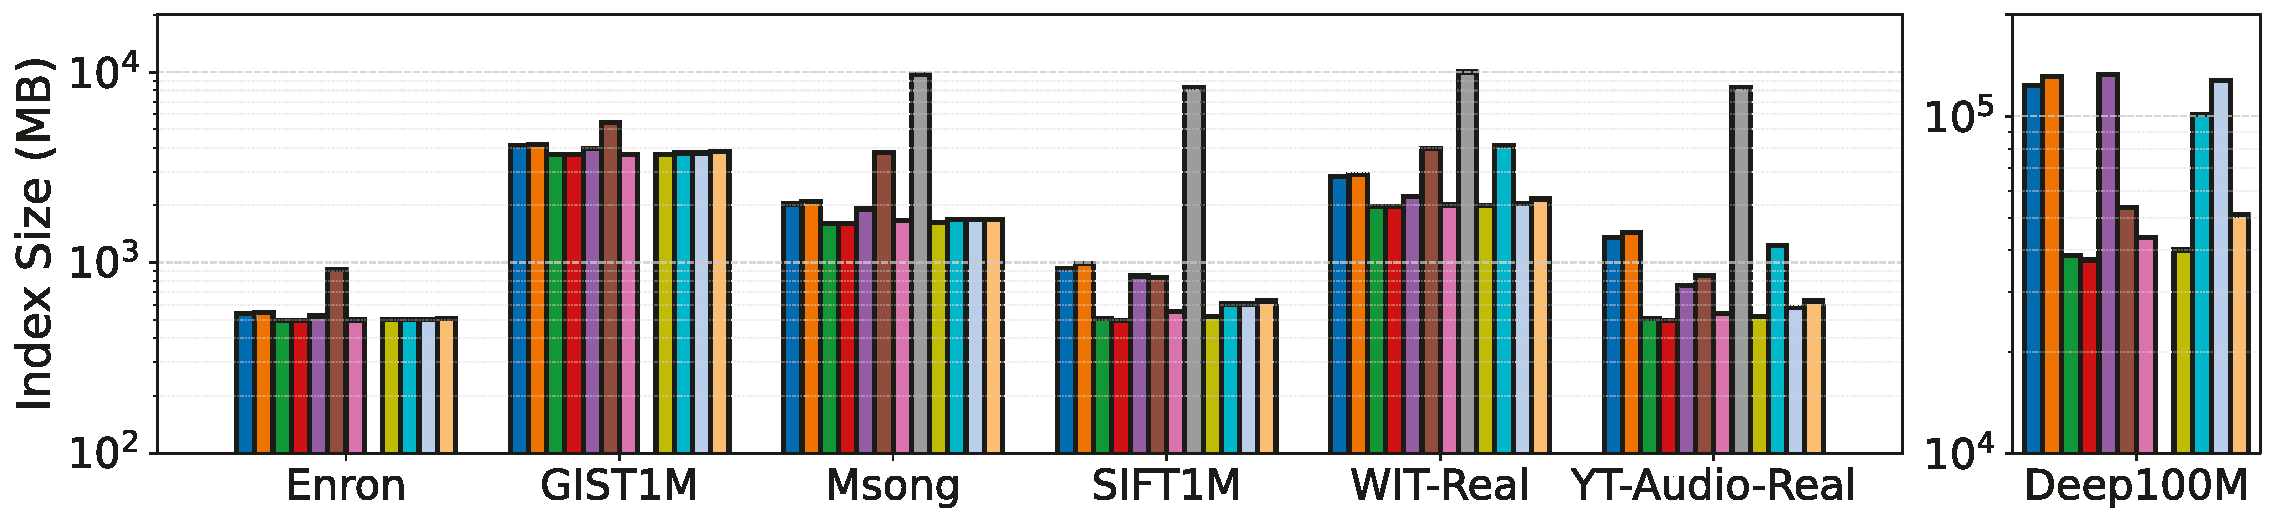
\includegraphics[width=0.99\linewidth]{figures/indexData/exp_7_index_size_mb_comparison_query1.pdf}
			\caption{Index Size (Including Original Dataset)}
			\label{fig:index_size_mb_comparison_query1}
		\end{subfigure}
		
		
		
		\begin{subfigure}{\columnwidth}
			\centering
			
			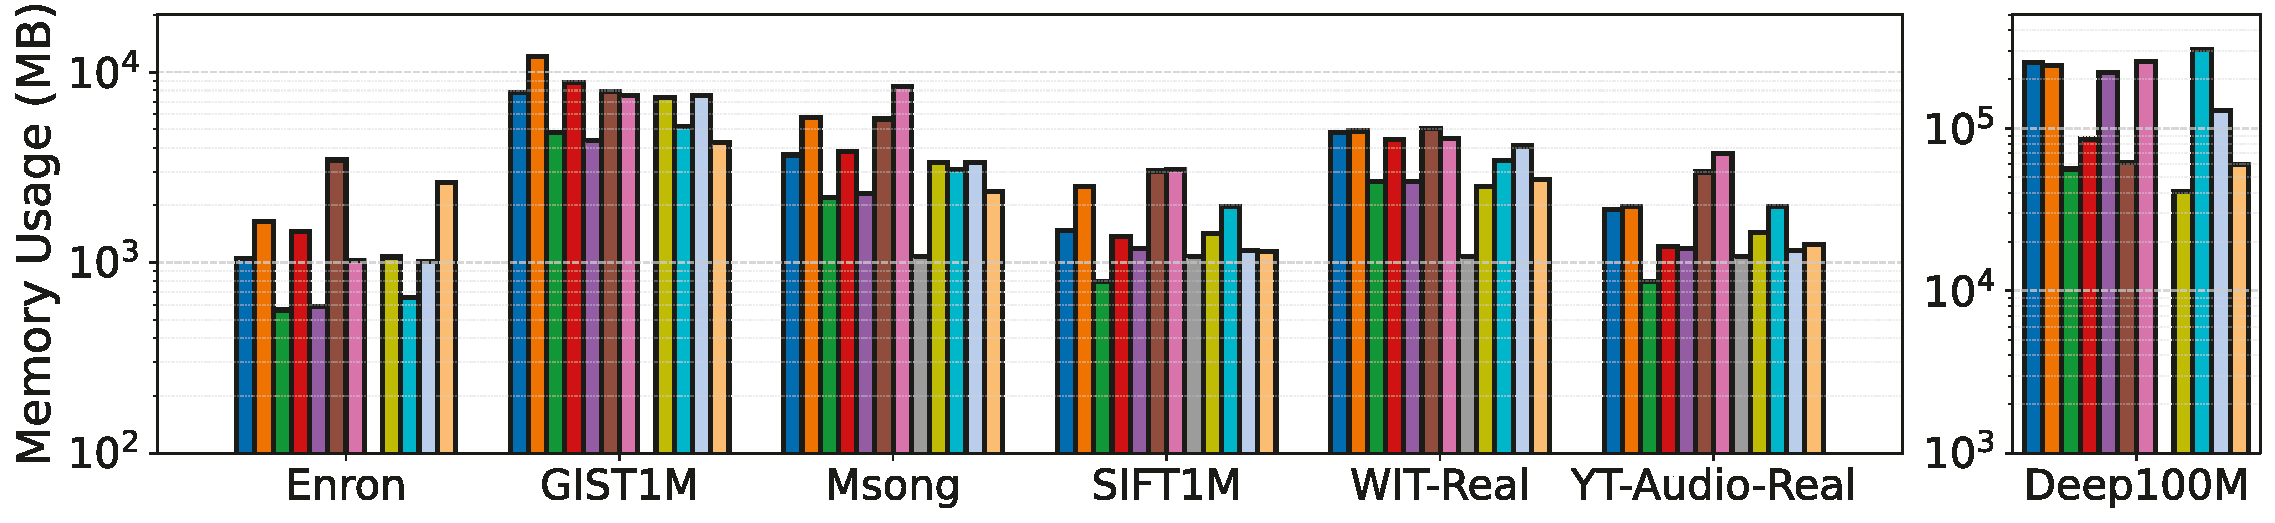
\includegraphics[width=0.99\linewidth]{figures/indexData/exp_7_memory_mb_comparison_query1.pdf}
			\caption{Build Peak Memory }
			\label{fig:build_memory_mb_comparison}
		\end{subfigure}
		
		\begin{subfigure}{\columnwidth}
			\centering
			
			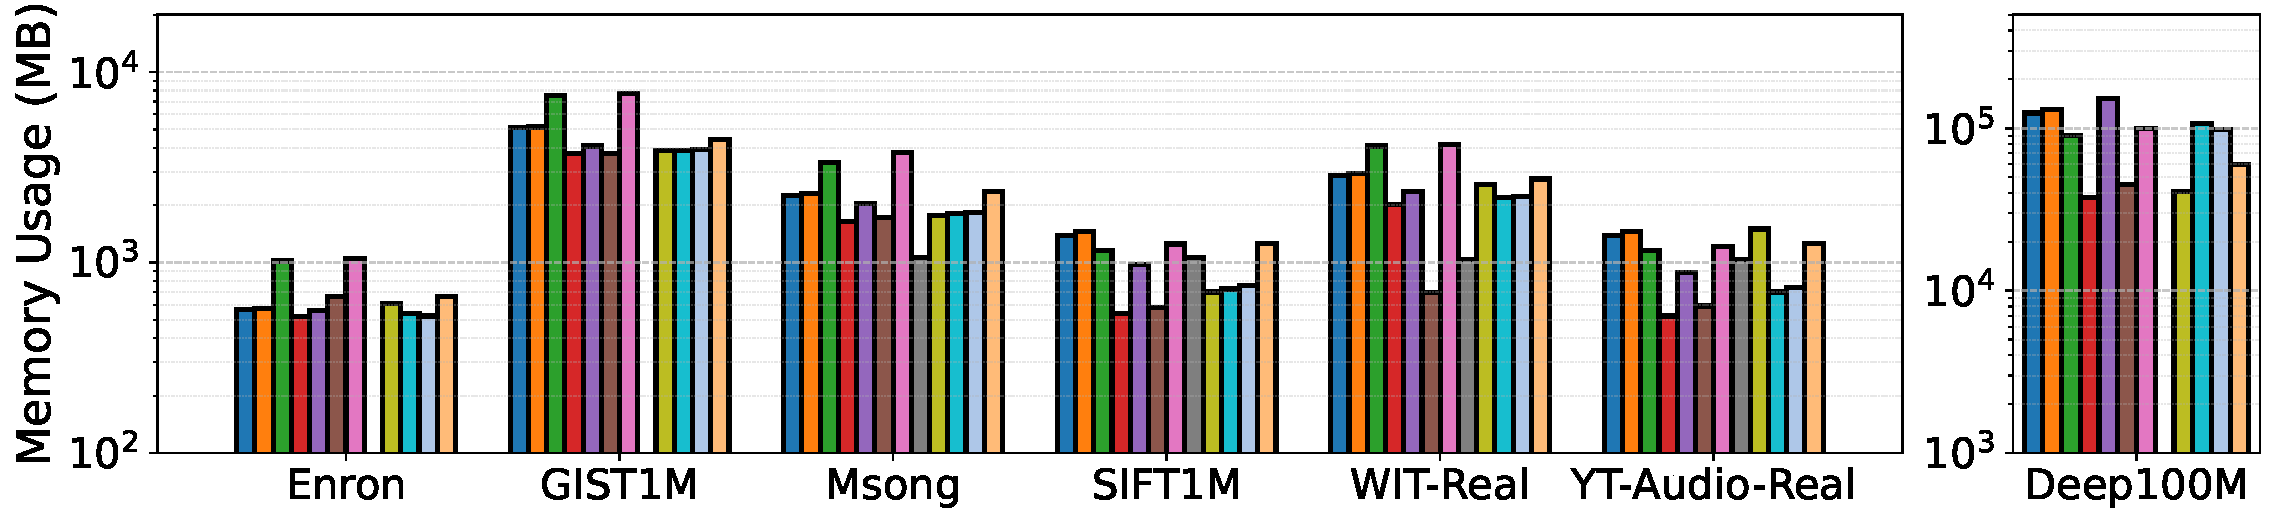
\includegraphics[width=0.99\linewidth]{figures/searchMem/label_memory_comparison.pdf}
			\caption{Search Peak Memory}
			\label{fig:search_memory_mb_comparison}
		\end{subfigure}
		
		%		\caption{Time and space overhead of attribute filtering index construction}
		\caption{\textcolor{violet}{Time and Space Overhead}}
		\label{fig:build_index_comparison}
	\end{figure}
	
	
	
	\textcolor{violet}{To investigate the time and space overhead of different algorithms,} we evaluate \textcolor{orange}{4} key metrics in the single-attribute scenario: index construction time, index size, \textcolor{orange}{build peak memory and search peak memory}. Notably, PASE on GIST1M and Enron is omitted, as it supports only data with dimensionality less than 512. \textcolor{orange}{Except for algorithms that only support single-threaded construction, all other algorithms are built using 32 threads on the 6 datasets shown in the left figure, and 64 threads on the large-scale Deep100M dataset.}
	
	
	\begin{figure*}
		\centering
		
		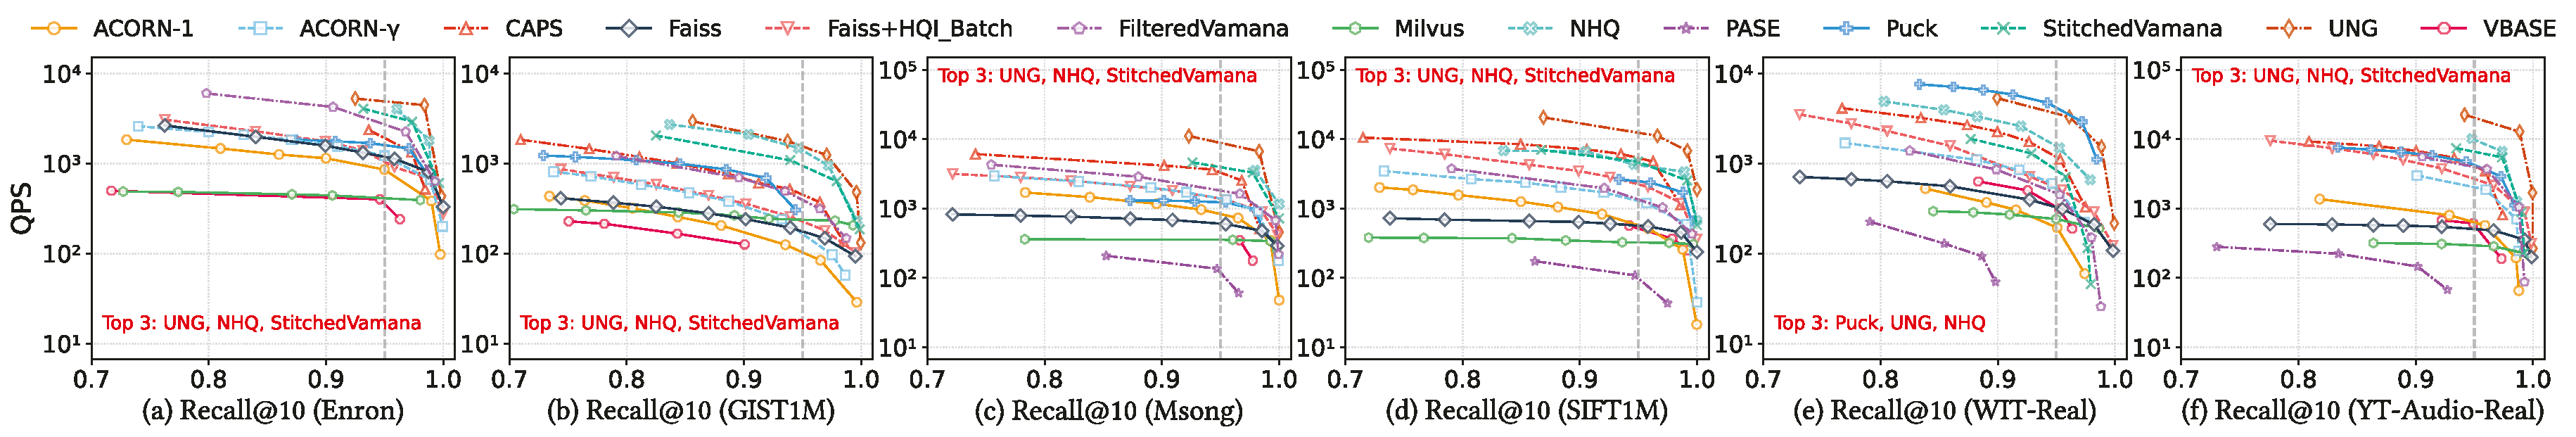
\includegraphics[width=0.95\textwidth]{figures/exp/exp_1_1_SingleLabel_1thread.pdf}
		\caption{Performance of Single-Attribute Index Construction and Single-Attribute Query (Single Thread) }
		\label{fig:exp_1_1_SingleLabel_1thread}
	\end{figure*}
	
	\begin{figure*}
		\centering
		
		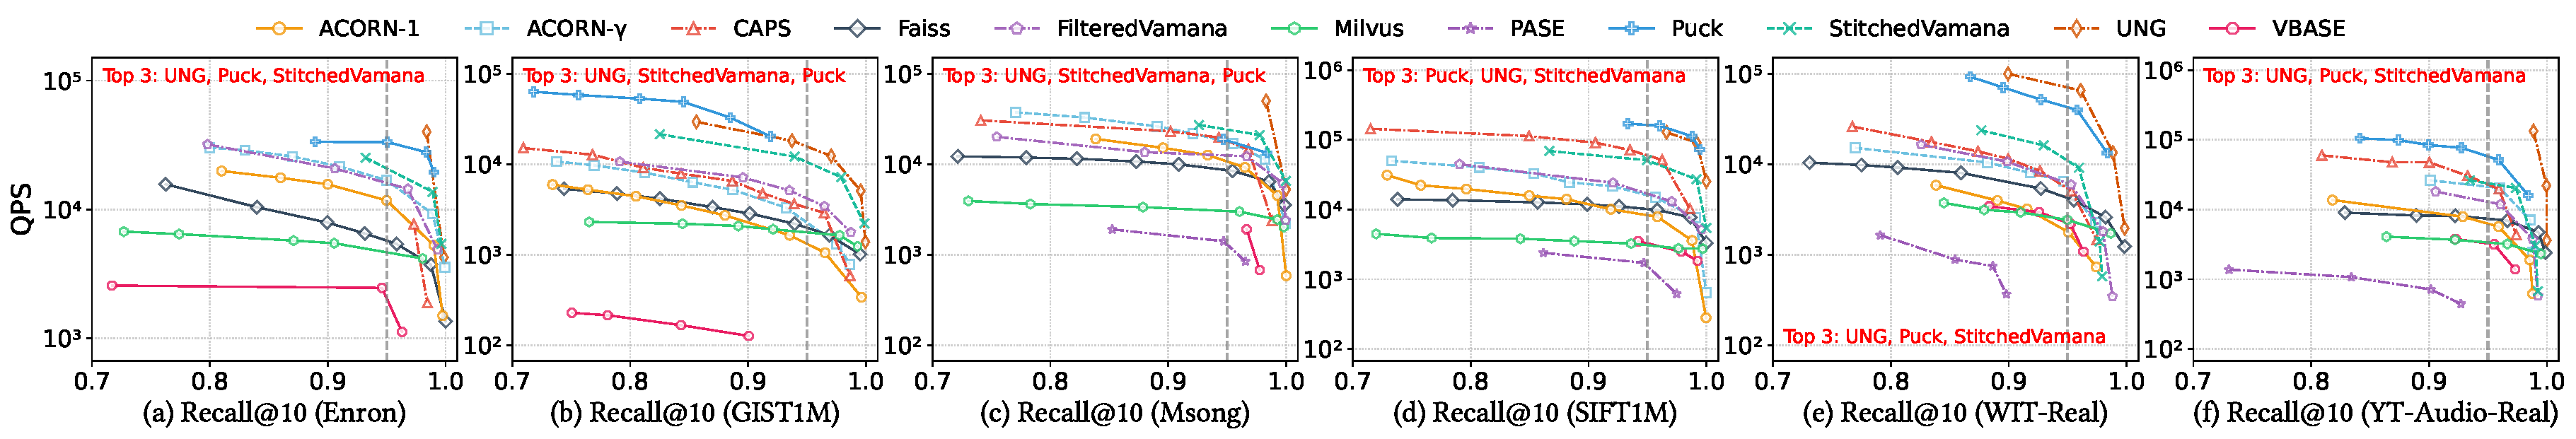
\includegraphics[width=0.95\textwidth]{figures/exp/exp_1_2_SingleLabel_16thread.pdf}
%		\caption{Single-Attribute Building and Query performance (16 threads)}
		\caption{Performance of Single-Attribute Index Construction and Single-Attribute Query (16 Threads)}
		\label{fig:exp_1_2_SingleLabel_16thread}
	\end{figure*}
	
\textit{\textbf{Index construction time.}}
\textcolor{orange}{Among the regular-scale datasets shown in the left part of Figure~\ref{fig:build_time_comparison_query1}, the methods with longer build times are mainly PASE, VBASE, and ACORN-$\gamma$. PASE and VBASE only support single-threaded builds, and PASE is the slowest because its on-demand loading and caching strategies frequently trigger disk I/O and page scheduling, which seriously affects efficiency; VBASE uses full-memory builds and is relatively faster. ACORN-$\gamma$  has a large computational overhead because it needs to expand the neighbor list and evaluate a large number of candidates. The build time on some datasets even exceeds that of single-threaded VBASE. }

\textcolor{orange}{On large-scale dataset Deep100M, besides the three methods already mentioned, we also observe that algorithms based on Vamana (such as FilteredDiskANN and UNG) exhibit significantly increased construction time. Vamana adopts a two-pass graph construction and optimization strategy (greedy search + robust pruning), resulting in extremely high computational overhead. 
In contrast, the construction time of IVF-based algorithms grows much more slowly with dataset size, thanks to their shard-based design and high parallel efficiency, making them more scalable and advantageous in large-scale scenarios.}

%ACORN-1 achieves the fastest index construction. This efficiency stems from its similarity to the original HNSW construction process and the use of a limited number of candidate neighbors.

%\textcolor{orange}{As shown in Figure~\ref{fig:build_time_comparison_query1}, in the above datasets, both PASE and VBASE are single-threaded indexing methods, with PASE having the longest construction time. The on-demand loading and caching strategy used by PASE results in frequent disk I/O and page scheduling, which significantly slow down the construction process. In contrast, VBASE uses full in-memory construction, leading to faster indexing.}
%
%
%For algorithms supporting 32-thread, ACORN-1 achieves the fastest index construction. This efficiency stems from its similarity to the original HNSW construction process and the use of a limited number of candidate neighbors. In contrast, ACORN-$\gamma$ incurs the highest index construction time, as it expands neighbor lists and evaluates a large candidate pool, leading to increased computational overhead. \textcolor{orange}{Its construction time on some datasets is even slower than that of the single-threaded VBASE.}
%
%On large dataset Deep100M, VBASE takes longer to build because it only supports single-threaded construction. The other time-consuming algorithms are all graph-based methods, which employ complex pruning strategies during construction to optimize query performance, leading to significantly increased build times.


\textit{\textbf{Index size.}}
\textcolor{orange}{
	As shown in Figure~\ref{fig:index_size_mb_comparison_query1}, PASE exhibits significantly larger index sizes across all supported datasets, mainly due to its reliance on a large amount of metadata. For regular-scale datasets, other methods show moderate variation. However, on large-scale dataset, Graph-based algorithms such as ACORN, FilteredDiskANN, and UNG tend to exhibit a sharp increase in index size, primarily due to the large number of candidate neighbors they maintain. Overall, IVF-based methods tend to produce more compact indexes.
}

%As shown in the Figure~\ref{fig:index_size_mb_comparison_query1}, PASE exhibits significantly larger index sizes across all supported datasets. This overhead stems primarily from its extensive metadata requirements. The index sizes of other methods show moderate variation.
%\textcolor{orange}{Among these, we observe a trend that IVF-based methods tend to produce more compact indexes compared to graph-based methods.}


%\underline{Faiss generates slightly smaller indexes due to its efficient index design}.
\textit{\textbf{Build peak memory.}}
% As shown in Figure~\ref{fig:build_memory_mb_comparison}, 
% %on small-scale datasets, all methods except NHQ exhibit low memory usage. 
% \textcolor{orange}{NHQ has the highest peak memory usage on almost all datasets.}
% This is because NHQ adopts the kgraph approach for index construction, which requires loading the entire graph data into memory and maintaining a complete graph structure, leading to relatively high memory overhead. 
% 
% On large-scale datasets, CAPS exhibits slightly lower memory usage compared to other algorithms. \textcolor{orange}{The reason is that CAPS avoids redundant storage and graph structure overhead through hierarchical partitioning and AFT, and achieves a compact, sparse and controllable index. }.
\textcolor{orange}{As shown in Figure~\ref{fig:build_memory_mb_comparison}, the build peak memory usage is generally correlated with the sum of the index size and the dataset size. Algorithms that consume more peak memory during construction typically produce larger index sizes, and this trend holds across different datasets. However, PASE breaks this pattern due to its on-demand loading strategy, resulting in peak memory usage even lower than the final index size.}

\textcolor{orange}{
In addition, NHQ generates a large number of candidate neighbors during the construction phase, but retains only a small subset for each point in the final index. This leads to high peak memory usage during construction, despite the relatively small size of the final index.}

\textit{\textbf{ \textcolor{orange}{Search peak memory.}}}
%  \textcolor{orange}{As shown in Figure~\ref{fig:search_memory_mb_comparison}, we can find that the peak memory usage of each algorithm during search does not differ significantly. Among them, CAPS and NHQ have relatively higher peak memory usage, while the peak memory usage of database is comparatively lower.}
%\textcolor{orange}{For most algorithms, the query phase requires loading both the index and the dataset into memory, so its peak memory usage is usually comparable to that of the construction phase. However, as shown in the Figure~\ref{fig:search_memory_mb_comparison}, CAPS exhibits significantly higher peak memory during querying due to the need to dynamically maintain large candidate sets. In contrast, Milvus has lower peak memory usage because it does not fully load the index and incurs additional metadata overhead during construction.
\textcolor{orange}{
Most algorithms load both the index and the dataset into memory during the build and query phases, and the construction process typically generates a large amount of temporary data. As a result, peak memory usage during querying is generally slightly lower than during construction. However, exceptions exist. As shown in Figure~\ref{fig:search_memory_mb_comparison}, CAPS incurs significantly higher peak memory usage during querying due to the need to dynamically maintain a large candidate set.}
	
	\subsubsection{Performance Evaluation}
	
	
	%4.2.2
	
	
	We next evaluate the query performance of AF-ANN search methods, focusing on 3 main scenarios.
	
	\textit{\textbf{Single-Attribute Index Construction and Single-Attribute Query.}}
	In this scenario, we construct the index using an attribute and apply filtering conditions on the same attribute.
	
	
	\textit{Single-Thread Search.}  
	\textcolor{violet}{As shown in Figure~\ref{fig:exp_1_1_SingleLabel_1thread}, under near-perfect recall (recall approaching 1) conditions, search often requires traversing larger candidate sets or deeper graph paths. This leads to increased computational cost and a sharp QPS drop for most methods. Despite this, UNG consistently maintains high QPS due to its LNG structure, which eliminates unnecessary online filtering of irrelevant attributes and searches only within the subgraph formed by points satisfying the filtering conditions, thereby improving query efficiency.}
	
	\textcolor{violet}{NHQ and StitchedVamana also perform well and show similar and stable performance across all datasets. This indicates that joint filtering and search strategies can achieve consistent effectiveness under high-recall requirements.}
	
	\textcolor{violet}{StitchedVamana outperforms FilteredVamana in query efficiency. This difference stems from their pruning strategies: StitchedVamana applies pruning after merging graphs, allowing nodes to accumulate a richer candidate set; while FilteredVamana applies early pruning, potentially eliminating useful candidates prematurely.}
	
	%	Puck and CAPS perform relatively well. Partition-based methods have limitations regarding different vector data distributions, and how to configure different partitions for different datasets remains a challenge. However, this also demonstrates that IVF-based methods remain very promising for hybrid queries.
	
	\textcolor{violet}{Puck and CAPS perform relatively well, indicating that IVF-based methods remain very promising for hybrid query.}
	
	\textcolor{violet}{Among all methods, vector database systems (PASE, VBASE, Milvus) show the worst performance. These systems target general-purpose scenarios but incur communication latency from network I/O and experience high query processing overhead due to complex query parsing. Additionally, we observe that Faiss+HQI\_Batch outperforms original Faiss, indicating that batch querying via HQI can effectively enhance query performance.}
	
	\textcolor{violet}{\textit{Multi-Thread Search.} As shown in Figure~\ref{fig:exp_1_2_SingleLabel_16thread}, under multi-threading, all algorithms except Puck show similar improvements, with UNG continuing to maintain the best performance. Puck achieves significant performance improvements in multi-threaded scenarios, delivering near-linear speedup by processing each query independently with a thread-local search context. This design eliminates synchronization overhead, enabling efficient parallel execution.}
	
	%	\textit{Single-Thread Search.}  
	%	As shown in Figure~\ref{fig:exp_1_1_SingleLabel_1thread}, under full-recall conditions (recall = 1), search often requires traversing larger candidate sets or deeper graph paths, leading to increased computational cost and a sharp QPS drop for most methods. Despite this, UNG maintains high QPS due to its LNG structure, which eliminates unnecessary online filtering of irrelevant attributes, thereby improving query efficiency. But, UNG slightly underperforms on high-LID datasets such as GloVe. In contrast, CAPS performs better on high-LID datasets but is more sensitive to dataset characteristics. CAPS leverages multi-level spatial partitioning and attribute filtering to efficiently explore sparse spaces, whereas UNG relies on structured attribute organization, which limits its adaptability to sparse high-dimensional distributions.
	%	
	%	NHQ, StitchedVamana, and FilteredVamana show similar and stable performance across all datasets. This indicates that joint filtering and search strategies can achieve consistent effectiveness under high-recall requirements. As observed in Figure~\ref{fig:exp_1_1_SingleLabel_1thread}, StitchedVamana outperforms FilteredVamana in query efficiency. The difference arises from their pruning strategies: StitchedVamana applies pruning after merging graphs, allowing nodes to accumulate a richer candidate set; while FilteredVamana applies early pruning, potentially eliminating useful candidates prematurely.
	%	
	%	Among all methods, vector database systems (PASE, VBASE, Milvus) perform the worst. These systems target general-purpose scenarios but incur communication latency from network I/O and experience high query processing overhead due to complex query parsing. Additionally, we observe that Faiss+HQI\_Batch outperforms original Faiss, indicating that batch querying via HQI can effectively enhance query performance.
	%	
	%	\textit{Multi-Thread Search.}
	%	As shown in Figure~\ref{fig:exp_1_2_SingleLabel_16thread}, UNG continues to achieve the best performance. 
	%	%Puck performs well on large-scale datasets, but its performance degrades on small datasets. Puck is tailored for large-scale scenarios, and optimizations such as two-level inverted indexing and hierarchical quantization introduce unnecessary overhead on small datasets. 
	%	Puck performs well on large datasets but degrades on smaller ones due to overhead from optimizations like two-level inverted indexing and hierarchical quantization. CAPS maintains a relatively high throughput under multi-threads but exhibits limited adaptability to different datasets. The vector distribution of the dataset affects the construction of its partitioned index.
	%	 ACORN performs poorly overall, primarily due to the sensitivity of its hyperparameter $\gamma$ to attribute selectivity. Without careful tuning based on dataset characteristics, it is challenging to construct an effective index.
	
	\textit{\textbf{Multi-Attribute Index Construction and Single-Attribute Query.}}
	In this scenario, the index is constructed using 8 attributes but applies filtering condition on only 1 attribute during the query.
	
	Faiss offers an ID filtering mechanism, it operates solely during query execution and does not influence index building. ACORN is   designed for single-attribute indexing. In database systems (VBASE, PASE, Milvus), 
	%\sout{when the system builds both B+ tree and vector indexes, queries typically utilize only the B+ tree.} 
	attributes do not participate in index construction.
	Hence, they are excluded from this comparison.
	
	\begin{figure}[t]
		\centering
		
		% 上面的图例,居中并可通过 hspace 调整左右位置
		\hspace*{15pt} % 可调整的参数,负值左移,正值右移,例如 -20pt 或 20pt
		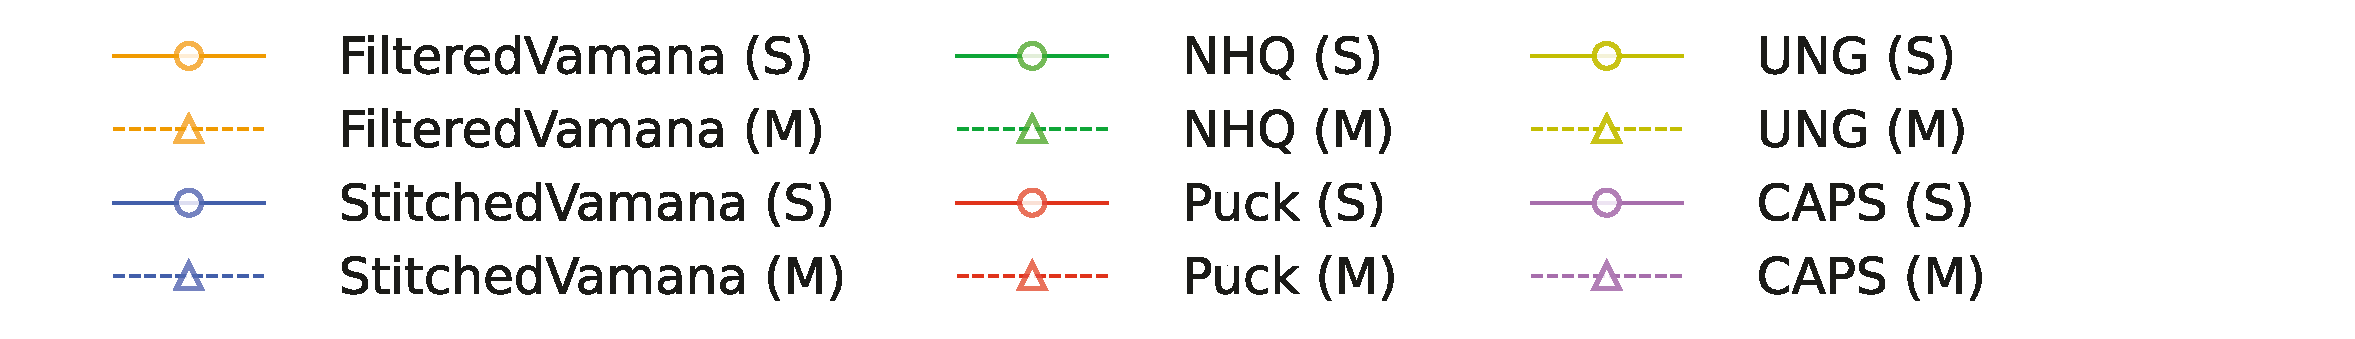
\includegraphics[width=0.85\columnwidth]{figures/exp/exp_2_legend.pdf} % 图例图片路径
		
		
		% 下面的子图,居中显示
		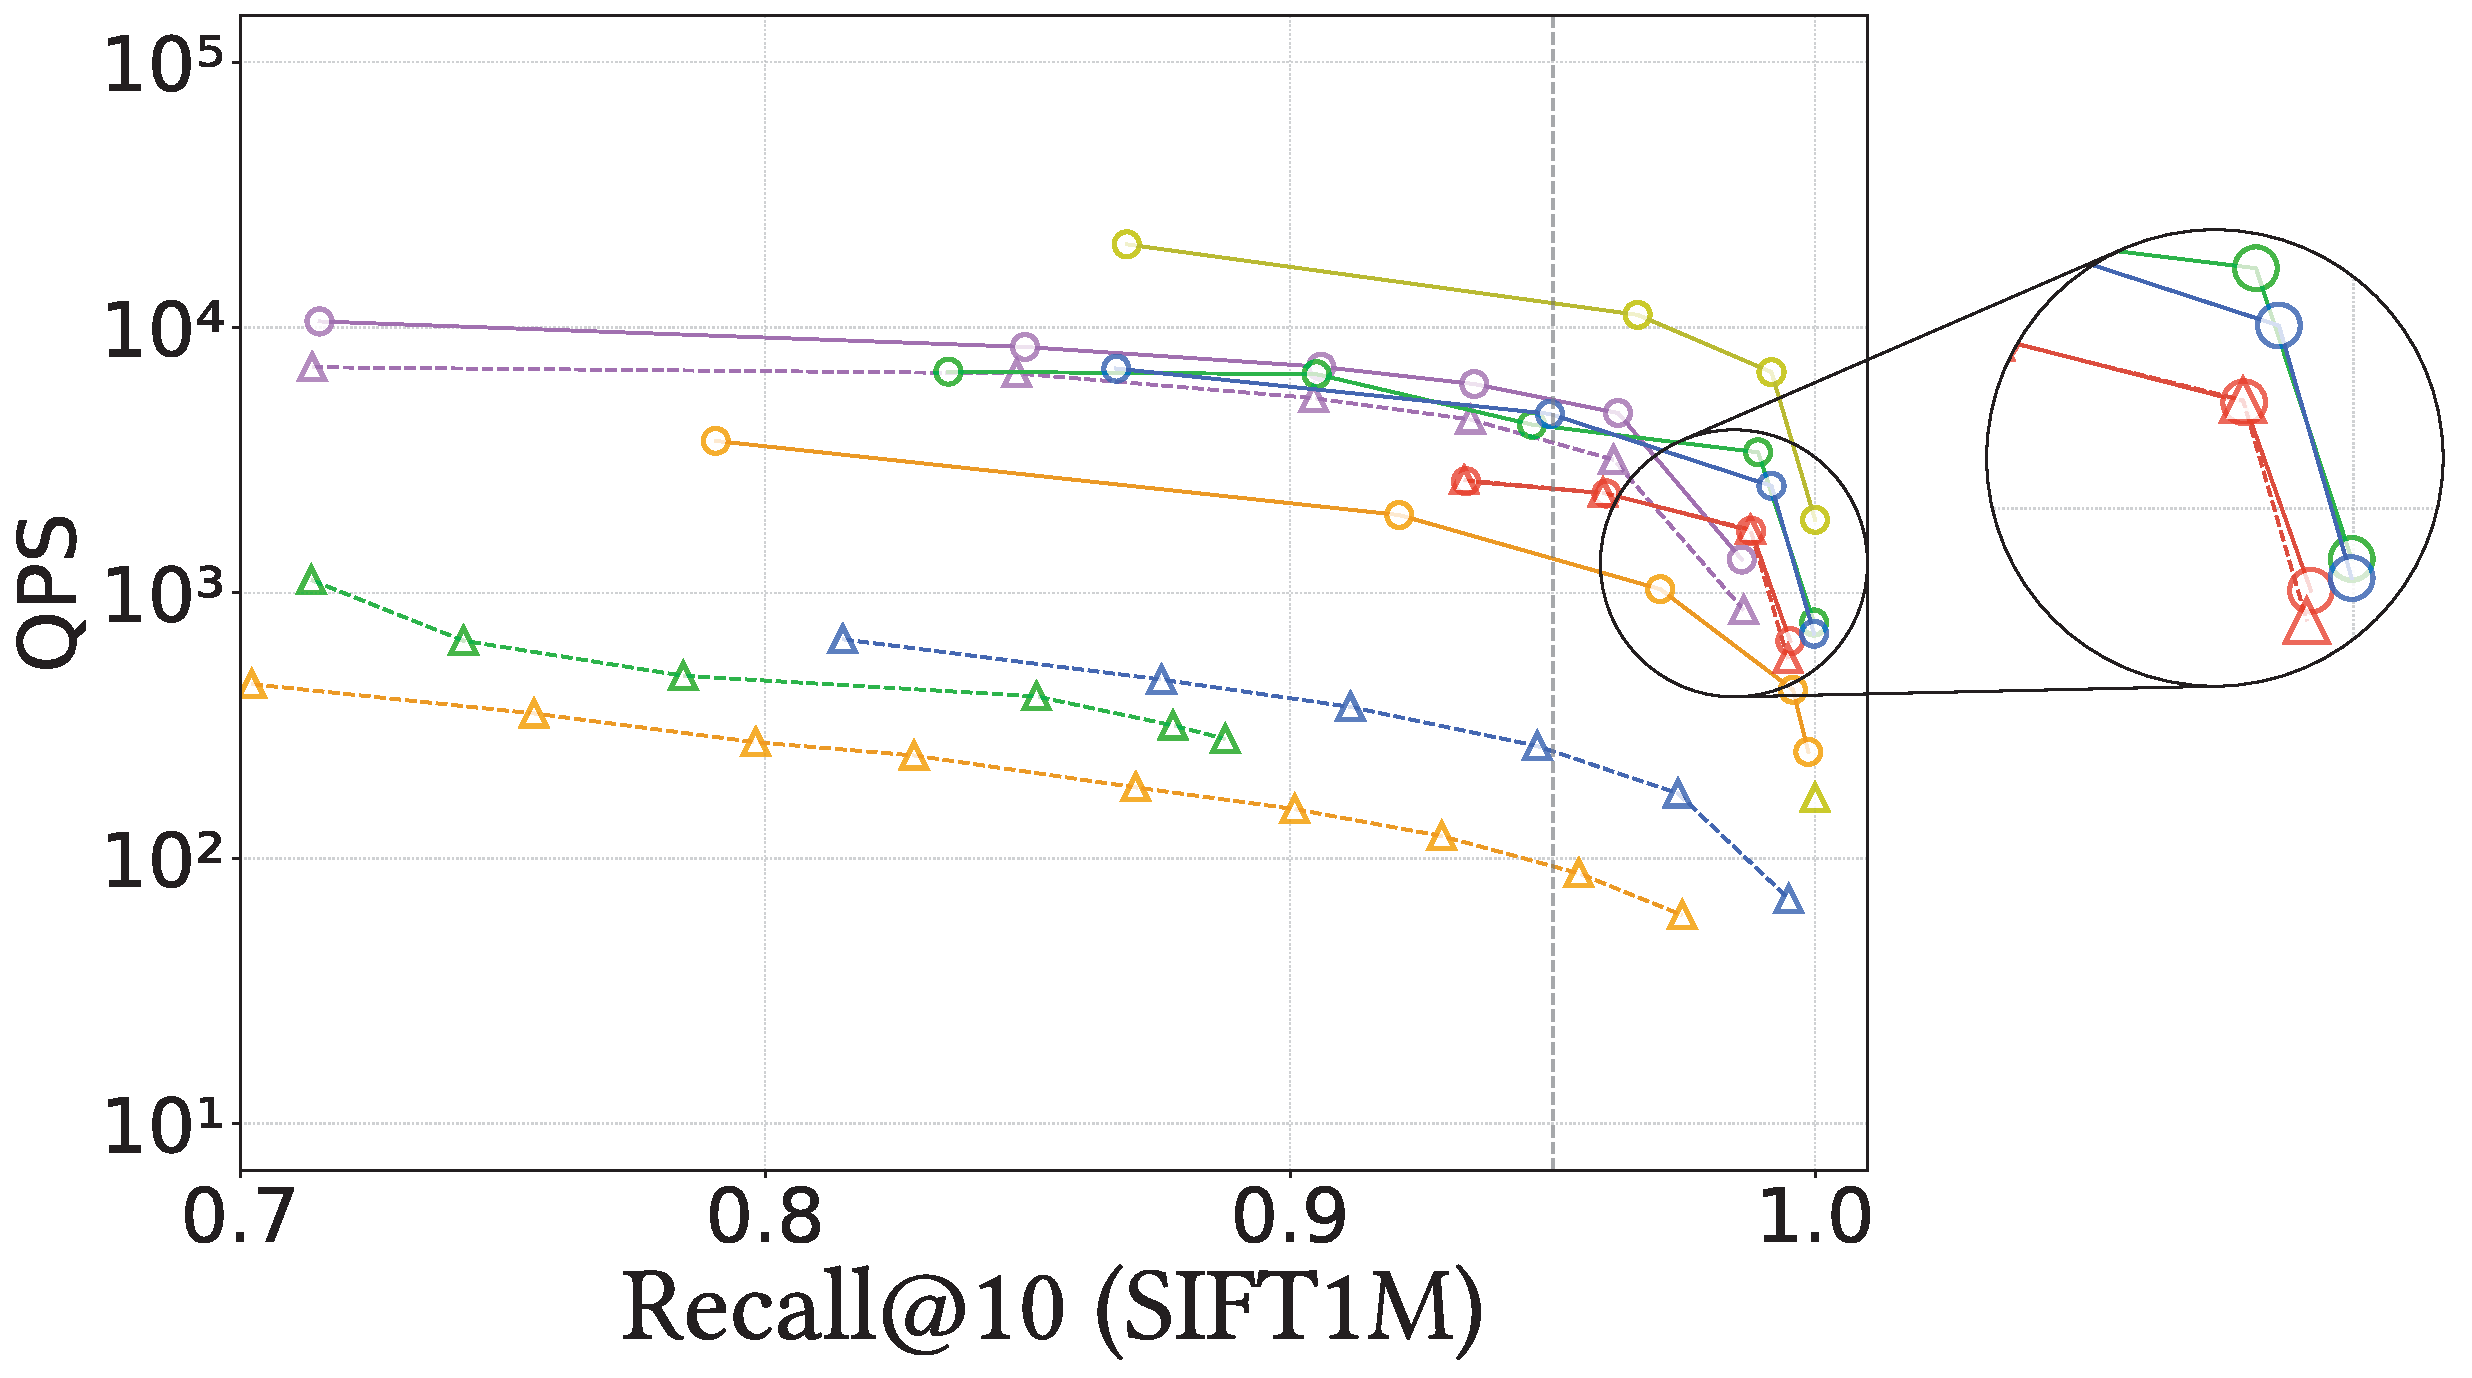
\includegraphics[width=0.7\columnwidth]{figures/exp/exp_2_1.pdf}
		\caption{Effect of Multi-Attribute Index Construction on Single-Attribute Query Performance ($S$ denotes single-attribute index construction and single-attribute query, $M$ denotes multi-attribute index construction and single-attribute query)}
		\label{fig:exp_2_1}
		
	\end{figure}
	
	\textit{Effect of Multi-Attribute Building on Algorithm Performance (M vs. S).}
	As shown in Figure \ref{fig:exp_2_1}, \textcolor{red}{Puck demonstrates nearly no performance degradation, because it accurately identifies the nearest clusters during a search, keeping the number of candidates constant, no matter how many attributes were used to build the index}. CAPS shows a slight performance decline due to the increased query overhead caused by excessive attribute-based grouping. In contrast, the performance of StitchedVamana, FilteredVamana, NHQ, and UNG drops significantly, with the following reasons: 1) FilteredVamana increases the complexity introduced by retaining attribute during index construction. 2) The complexity of StitchedVamana increases because data points may duplicate across multiple subgraphs. 3) The fusion distance of NHQ exhibits sensitivity to the number of attributes, which degrades its effectiveness. 4) UNG has poor performance because large number of entry points that need to be traversed. It is difficult for a graph with multiple entries to have good connectivity, degenerating into a situation closer to inverted retrieval, and the effect may be greatly impaired.
	
	
	
	\textit{Performance of Algorithms under Multi-Attribute Building (M vs. M).}  
	As shown in Figure \ref{fig:exp_2_1}, IVF-based methods (Puck and CAPS) significantly outperform graph-based methods. The reason for the superior performance of Puck is that it filters out irrelevant results during the retrieval process rather than searching for more candidates. CAPS performs as well as Puck. In contrast, FilteredVamana performs the worst because its multi-attribute indexing forces neighbor selection to cover multiple attributes, reducing the efficiency of single-attribute queries. This results in excessive traversal of irrelevant nodes, making it slower than other methods.
	
	
	\begin{figure*}
		\centering
		
		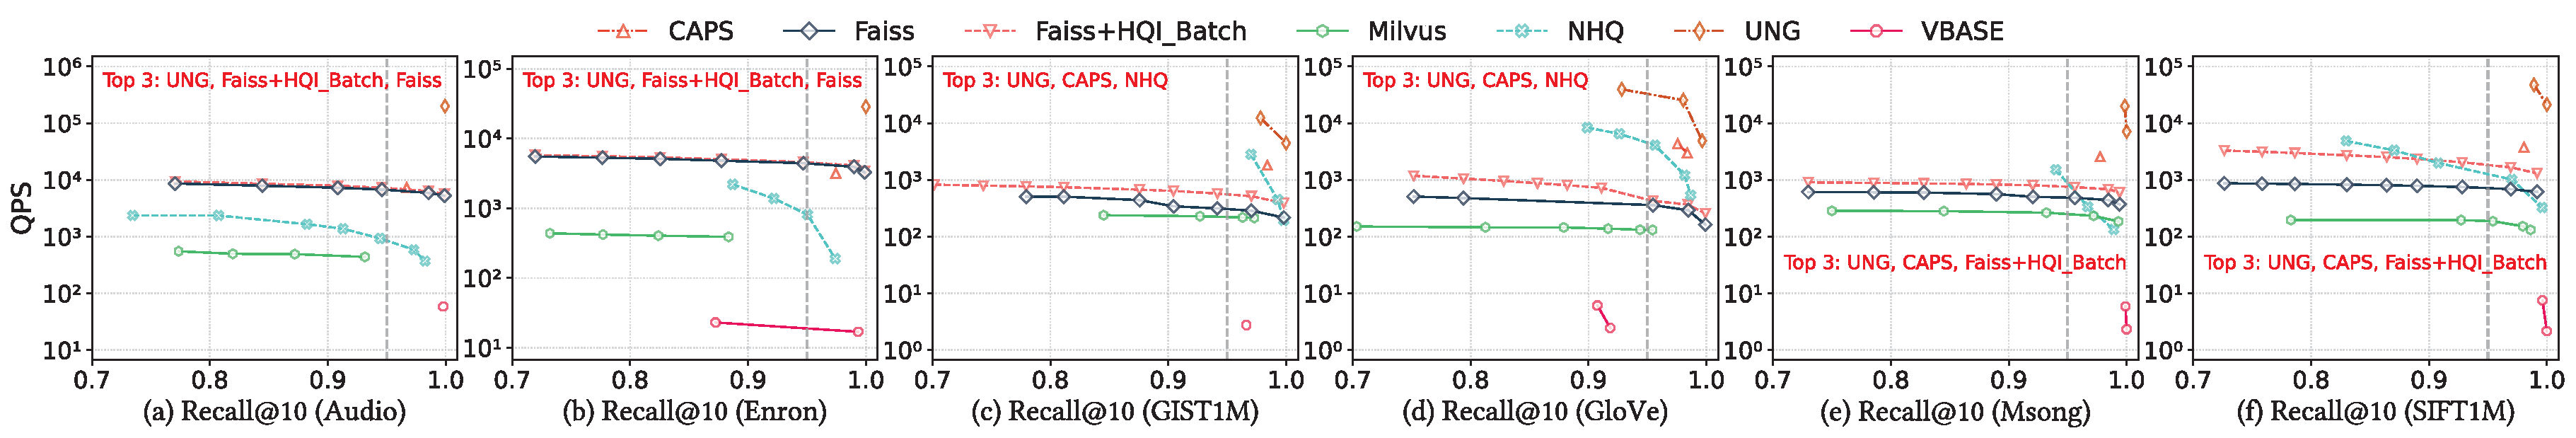
\includegraphics[width=0.95\textwidth]{figures/exp/exp_4_1_MultiLabel_1thread.pdf}
		\caption{Performance of Multi-Attribute Index Construction and Multi-Attribute Query}
		\label{fig:exp_4_1_MultiLabel_1thread}
	\end{figure*}
	
	
%	\begin{figure*}
%		\centering
%		
%		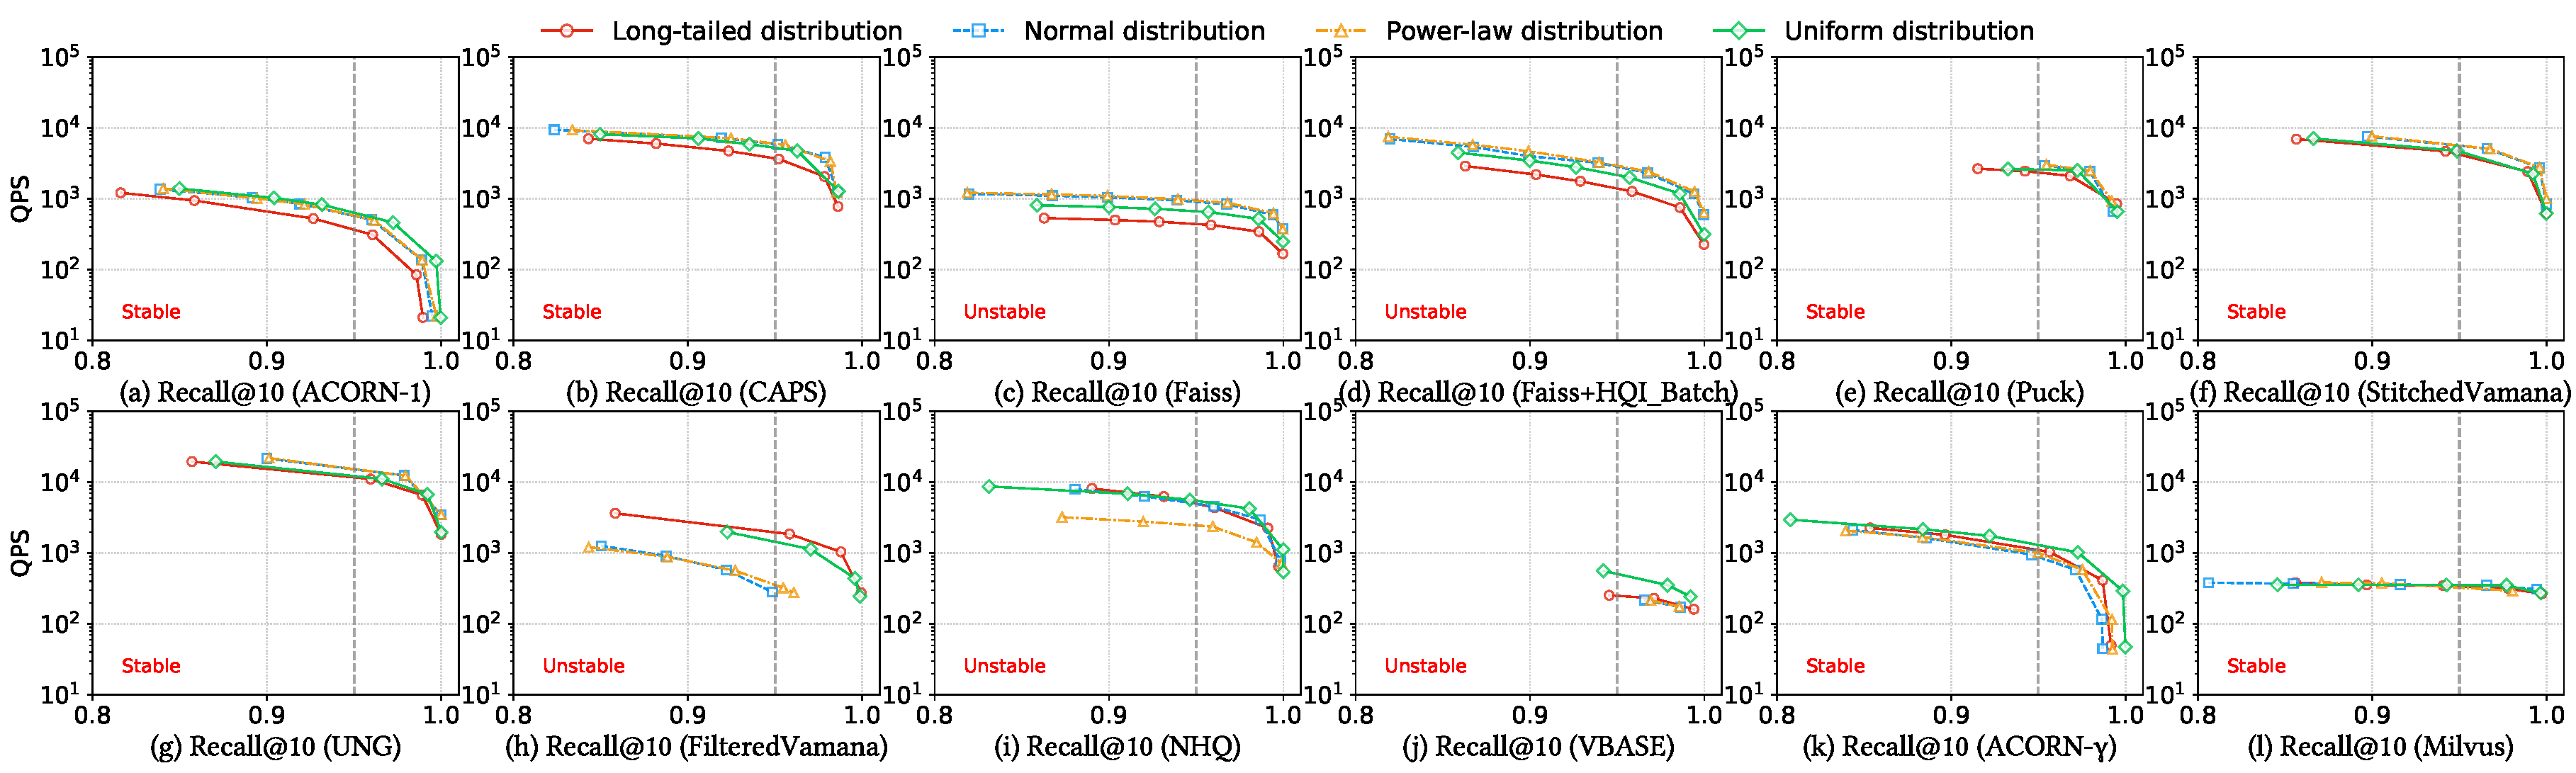
\includegraphics[width=0.95\textwidth]{figures/exp/exp_3_1.pdf}
%		\caption{Effect of Attribute Distribution on Query Performance (Strong is robust to attribute distribution shifts, Weak is sensitive to attribute distribution shifts)}
%		\label{fig:exp_3_1}
%		
%%		\footnotesize{
%%		\begin{center}
%%			\begin{minipage}{\linewidth}
%%				\centering	
%%				\textit{Strong} : robust to attribute distribution shifts,  \textit{Weak} : sensitive to attribute distribution shifts
%%			\end{minipage}
%%		\end{center}
%%		}
%	\end{figure*}
	
	
	
	
	
	\textit{\textbf{Multi-Attribute Index Construction and Multi-Attribute Query.}}  
	Compared to single-attribute filtering, multi-attribute joint filtering better reflects real-world scenarios. To evaluate algorithm performance under this setting, we construct the index using 3 uniformly distributed attributes and apply filtering on all 3 attributes simultaneously during queries. \textcolor{violet}{In this experiment, we only evaluate algorithms that support this multi-attribute query scenario.}
	
	As shown in Figure~\ref{fig:exp_4_1_MultiLabel_1thread}, UNG still maintains the best performance across all datasets. Since some strong competing algorithms do not support multi-attribute querying, CAPS becomes the second-best algorithm, but its performance on small datasets is relatively poor. This is because CAPS performs multi-level partitioning based on attributes on top of the IVF index, which introduces additional overhead. While this overhead negatively impacts performance on small datasets, on large datasets, the overhead is amortized, and the increasing dataset scale makes the advantages of attribute-aware partitioning evident.
	
	NHQ performs moderately overall in multi-attribute joint filtering scenarios but poorly on small datasets. Its reliance on fusion distance computations makes it highly sensitive to the number of attributes, impacting both efficiency and accuracy under multi-attribute filtering.
	
	For IVF-based methods not specifically optimized for hybrid queries (Faiss and Milvus), their QPS shows a similar and relatively stable trend as recall varies. Among them, Milvus, as a general-purpose system, exhibits comparatively poor performance.
	
%	Compared to single-attribute filtering, multi-attribute joint filtering better reflects real-world scenarios. To evaluate algorithm performance under this setting, we construct the index using 3 uniformly distributed attributes and apply filtering on all 3 attributes simultaneously during queries. \textcolor{orange}{Note that FilterDiskANN only supports Boolean OR logic and does not support Boolean AND. Therefore, its two Vamana-based methods are excluded from the multi-attribute construction and search experiments.}
%	%	\textcolor{red}{As Filtered-DiskANN does not support the AND rule used in our multi-attribute queries, it is excluded.}
%	%	Compared to single-attribute filtering, multi-attribute joint filtering better reflects real-world application scenarios. To evaluate algorithm performance under such scenario, we construct the index using 3 uniformly distributed attributes and apply filtering conditions on all 3 attributes simultaneously during the query process.
%	
%	As shown in Figure~\ref{fig:exp_4_1_MultiLabel_1thread}, UNG achieves the best performance across all datasets. For IVF-based methods not specifically optimized for hybrid queries (Faiss\_IVF and Milvus), their QPS remains relatively stable as recall varies. Milvus, as a general-purpose system, exhibits comparatively poor performance. 
%	
%
%	The IVF-based algorithm Faiss---especially when combined with HQI\_Batch---achieves moderate performance. It naturally supports pre-filtering and remains unaffected by the increasing number of attributes. In fact, filtering can reduce the effective candidate set, thereby improving search efficiency. In contrast, the IVF-based algorithm CAPS, which is optimized for hybrid queries, employs a multi-level partitioning strategy that introduces additional overhead. This overhead negatively impacts performance on small datasets. However, on large datasets, the overhead is amortized, and the advantages of attribute-aware partitioning become evident, making CAPS the second-best performer after UNG.
%	
%	NHQ performs moderately overall but poorly on small datasets. Its reliance on fusion distance computations makes it highly sensitive to the number of attributes, impacting both efficiency and accuracy under multi-attribute filtering.
	
	
	
	%	In contrast, Faiss—especially when combined with HQI\_Batch—achieves medium-level performance. Its original IVF implementation naturally supports pre-filtering and does not suffer from the complexity introduced by an increased number of attributes. In fact, filtering can reduce the effective candidate set, improving efficiency.
	%	As shown in Figure~\ref{fig:exp_4_1_MultiLabel_1thread}, UNG achieves the best performance across all datasets. For IVF-based methods that are not specifically optimized for hybrid query scenarios (Faiss\_IVF and Milvus), their QPS remains relatively stable as the recall varies. Milvus, being a general-purpose system, exhibits comparatively poor performance. In contrast, Faiss—especially when combined with HQI\_Batch—achieves medium-level performance. Its original IVF implementation naturally supports pre-filtering and does not suffer from the complexity introduced by an increased number of attributes. In fact, filtering can reduce the effective candidate set, improving efficiency.
	
	%	The IVF-based algorithm CAPS, optimized for hybrid queries, employs a multi-level partitioning strategy that introduces additional overhead. This overhead negatively impacts performance on small datasets. However, on large datasets, the overhead is amortized, and the benefits of attribute-aware partitioning become evident, making CAPS the second-best performer after UNG.
	
	%	NHQ exhibits mediocre performance overall and performs particularly poorly on small datasets. It relies on fusion distance calculations. The fusion distance computation is highly sensitive to the number of attributes involved, thus impacting both efficiency and accuracy under multi-attribute filtering.
	
	
	
	
	\subsubsection{Robustness}In the following, we evaluate the robustness of these algorithms.
	
%	\textit{\textbf{Attribute Distribution.}} To evaluate performance across different attribute distributions, we generate base and query attribute sets with 4 representative distributions—long-tailed, normal, power-law, and uniform—across the 6 datasets described in Section~4.1.1. We evaluate all algorithms under these distributions on each dataset. The performance differences observed for the same algorithm across different datasets are relatively minor. Thus, due to space constraints, we present only the results on SIFT1M.
%	
%	As illustrated in Figure~\ref{fig:exp_3_1}, the evaluated algorithms exhibit varying degrees of sensitivity to attribute distribution shifts. \textcolor{cyan}{The proximity of the 4 curves in the figure reflects algorithm sensitivity to distributional variations. When the curves converge closely, the algorithm demonstrates strong resilience against attribute distribution shifts.} Specifically, ACORN, Milvus, Puck, CAPS, StitchedVamana, and UNG demonstrate strong robustness to such shifts. In contrast, Faiss, FilteredVamana, NHQ, VBASE, and PASE show notable sensitivity.
%	
%	{\color{blue}{
%		Algorithms that are highly sensitive to attribute distribution tend to rely passively on the statistical characteristics of the attributes in their design. For instance, graph-based indexing methods like FilteredVamana and NHQ are prone to degraded connectivity or distorted structures under power-law distributions, where label frequencies are highly imbalanced. Similarly, VBASE, which employs a post-filtering strategy, shows efficiency that directly correlates with attribute selectivity—the more selective the filter, the more computational resources are wasted on retrieving irrelevant vectors. Faiss, which searches within the nearest clusters, may need to traverse more clusters to find sufficient results when relevant data points are unevenly distributed across clusters due to attribute skew, which impacts performance.
%		
%		In contrast, algorithms with low sensitivity to attribute distribution incorporate smarter indexing designs or adaptive query strategies to mitigate these challenges. Milvus, for example, leverages a built-in query optimizer that dynamically determines whether to filter by attributes or search vectors first, based on the selectivity of the query, thus ensuring more robust performance. Other approaches enhance robustness by separating attribute and vector indexing into distinct stages: UNG uses a logical graph to navigate attribute relationships, while CAPS employs an attribute frequency tree to adapt to power-law patterns. In ACORN--\(\gamma\), during index construction, attributes are primarily used for pruning in the lowest-layer graph, while the upper-layer hierarchical navigation graphs remain largely unaffected. Consequently, changes in attribute distribution have minimal impact on overall performance.}}
		
%	Among all algorithms, ACORN-\(\gamma\) shows the highest robustness. During index construction, attribute is mainly used for pruning in the lowest layer graph, while the upper-layer hierarchical navigation graphs remain largely unaffected. As a result, changes in attribute distribution have a limited impact on overall performance.
%	
%	\textcolor{cyan}{In contrast, FilteredVamana achieves optimal performance under long-tail and uniform distributions, as these enable construction of balanced label subgraphs with minimal inter-label interference, thus improving search accuracy and efficiency. However, its performance declines under power-law and normal distributions: power-law distributions cause excessive concentration of popular labels and fragmentation of niche labels, disrupting search path connectivity, while normal distributions produce ambiguous graph structures due to label frequency similarities, leading to search divergence. 
%	Under the power-law distribution, when the NHQ algorithm constructs an index based on fusion distance, points corresponding to high-frequency attribute values make the graph connections extremely dense, while points corresponding to low-frequency attribute values tend to become isolated due to sparse connections. This extreme imbalance in connectivity severely distorts the structure of the graph, ultimately significantly impairing the overall performance of the algorithm.
%	The search performance of VBASE exhibits a direct dependence on attribute selectivity. As selectivity decreases, search speed declines. Notably, only uniform distribution maintains sufficient selectivity among the tested cases; the other three distributions consistently show low selectivity levels that significantly degrade the operational efficiency of VBASE.}
	
%	\begin{figure}
%		\centering
%		\setlength{\abovecaptionskip}{0.1cm}
%		\setlength{\belowcaptionskip}{-0.1cm}
%		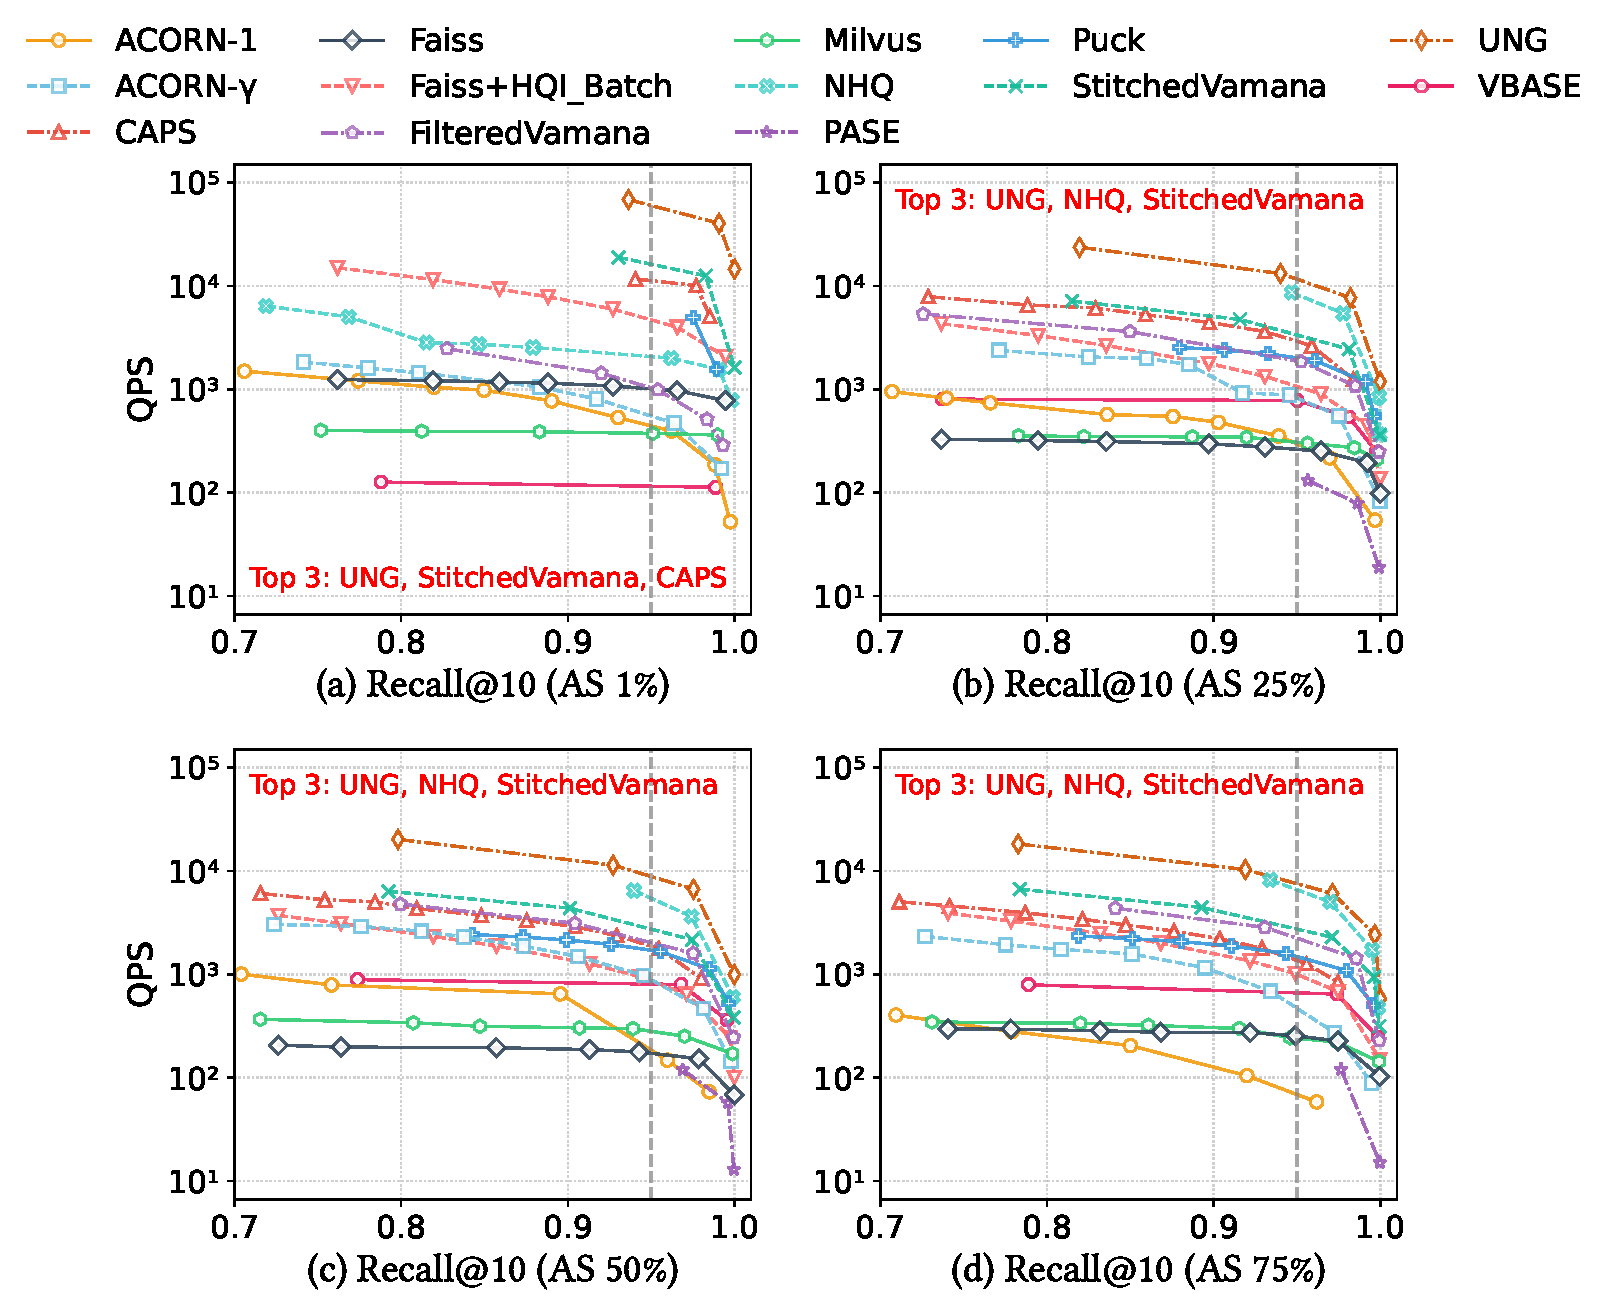
\includegraphics[width=0.95\columnwidth]{figures/exp/exp_5_1_1_SingleLabel_1thread.pdf}
%		\caption{Effect of Single-Attribute Selectivity on Query}
%		\label{fig:exp_5_1_1_SingleLabel_1thread}
%	\end{figure}
	
	
	\textit{\textbf{Single-Attribute Selectivity.}}
	In hybrid queries, varying attribute selectivity (AS) can significantly impact computational cost and query efficiency, as the algorithm must efficiently identify data points matching specific attributes within large datasets. AS is defined as the proportion of data points sharing a given attribute value. For example, AS of 1\% indicates that only 1\% of the dataset meets the given attribute. 
	
	To investigate this effect, we evaluate 4 AS settings (1\%, 25\%, 50\%, and 75\%) on the SIFT1M dataset using single-thread execution. 
%	We compare the query performance of attribute filtering algorithms across these settings, as shown in Figure~\ref{fig:exp_5_1_1_SingleLabel_1thread}.
	Based on the query performance trends of different algorithms under varying AS, we categorize the algorithms into 3 groups:
	
%	Experimental results show that UNG achieves the best performance across all AS settings, especially at extremely low AS (1\%). 
%	This advantage stems from its pre-filtering strategy. Pre-filtering strategy significantly reduces the ANN search space by narrowing down candidates prior to vector computation. In contrast, VBASE performs the worst at 1\% AS due to its post-filtering strategy. Post-filtering strategy first retrieves a large number of candidates and then applies filtering, incurring substantial computational overhead.
	
	
	
	
	\begin{figure*}
		\centering
		
		% 第一行:单独一张大图
		\begin{subfigure}{\textwidth}
			\centering
			
			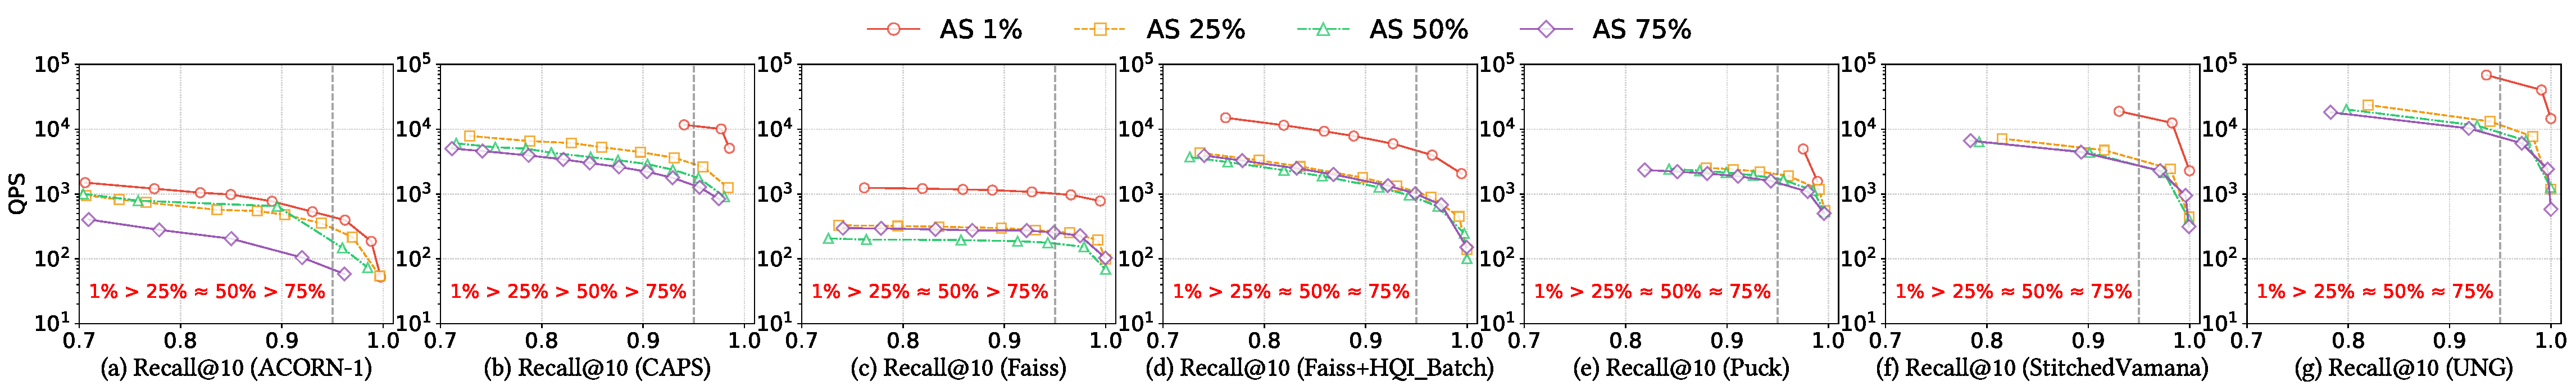
\includegraphics[width=0.95\textwidth]{figures/exp/exp_5_2_1.pdf}
			\caption{Algorithms Optimized for Low AS}
			\label{fig:exp_5_2_1}
		\end{subfigure}
		
		\vfill % 增加垂直间距
		
		% 第二行:两张子图,左侧宽度是右侧的两倍
		\begin{subfigure}{0.627\textwidth} % 2/3 宽度
			\centering
			
			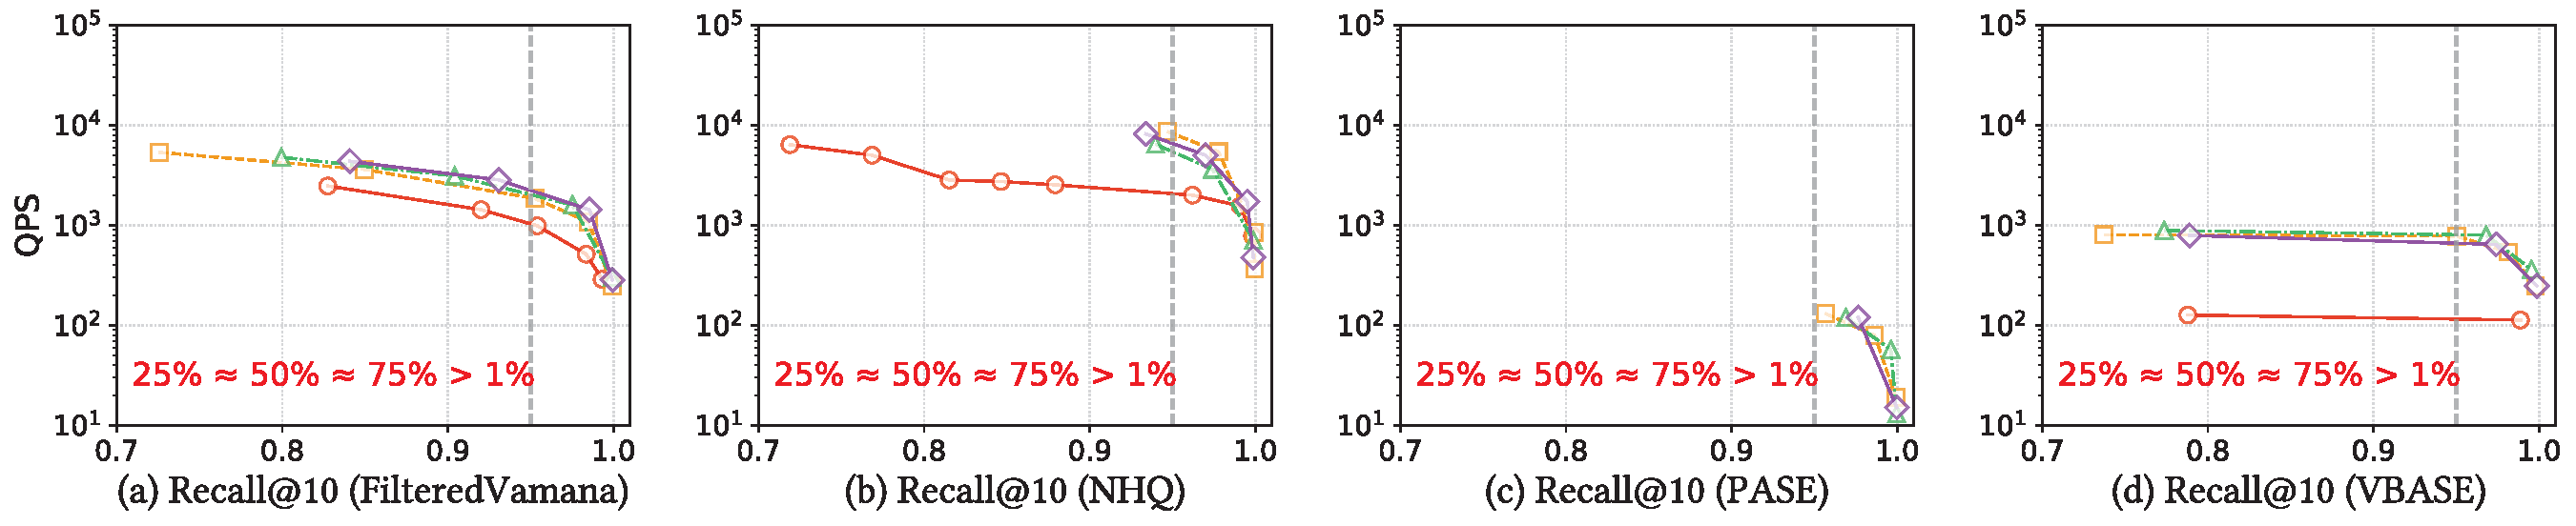
\includegraphics[width=0.96\textwidth]{figures/exp/exp_5_2_2.pdf}
			\caption{Algorithms Optimized for High AS}
			\label{fig:exp_5_2_2}
		\end{subfigure}
		\hspace{1mm} % 增加水平间距
		\begin{subfigure}{0.33\textwidth} % 1/3 宽度
			\centering
			
			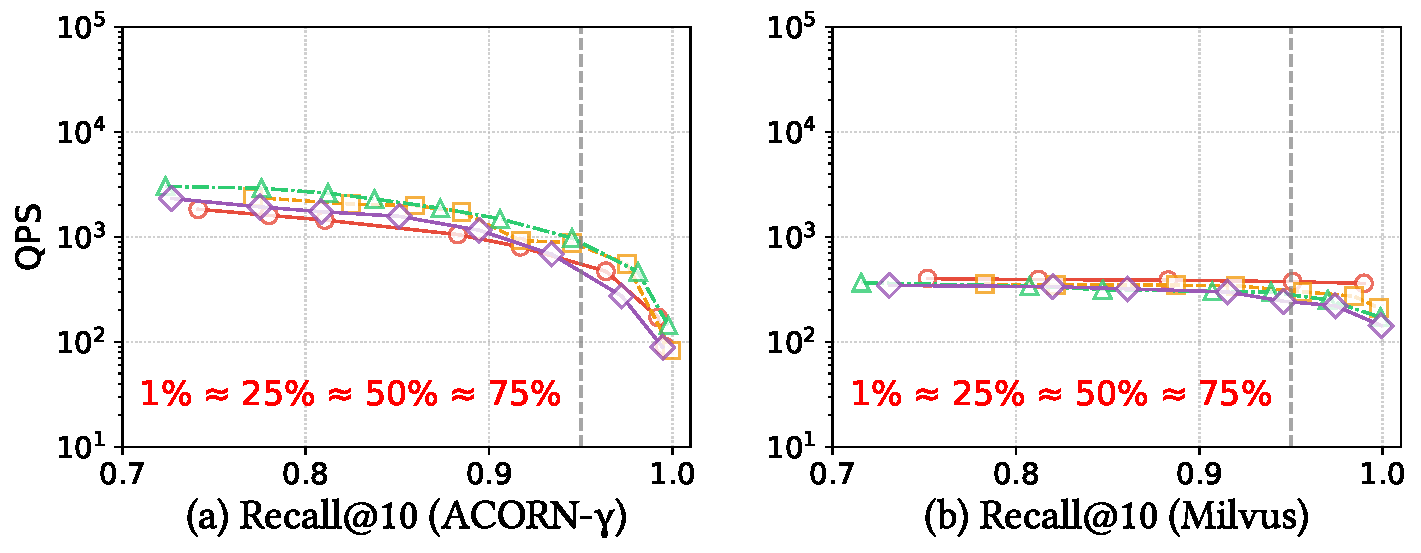
\includegraphics[width=0.96\textwidth]{figures/exp/exp_5_2_3.pdf}
			\caption{Algorithms Insensitive to AS}
			\label{fig:exp_5_2_3}
		\end{subfigure}
		
		
		\caption{Different AS under the Same Algorithm}
		\label{fig:exp_5_2_combined}
	\end{figure*}
	
	
	
	
	(1) \textit{Algorithms optimized for low AS.}  
%	This group includes ACORN-1, CAPS, Faiss, Faiss+HQI\_Batch, Puck, StitchedVamana and UNG, as illustrated in Figure~\ref{fig:exp_5_2_1}.
	\textcolor{orange}{Figure~\ref{fig:exp_5_2_1} shows the algorithms suitable for low AS.}
	\textcolor{orange}{ACORN-1}, Faiss, Puck and UNG all use pre-filtering strategies to shrink the search space in low AS, leading to better performance. \textcolor{orange}{Pre-filtering strategies significantly reduce the number of candidate points under low AS, thereby lowering the cost of  computations. As a result, such strategies tend to perform better in low AS scenarios.}CAPS efficiently skips irrelevant subpartitions, reducing computational overhead. However, as AS increases, it must process more subpartitions and handle a larger dataset. StitchedVamana optimizes local adjacency using independent subgraphs, enabling fast localization at low AS. However, at higher AS, it requires broader global exploration. 
	
%	ACORN-1 performs well in low AS because fewer nodes share the same attribute. This increases the average degree of retained nodes and improves graph connectivity. UNG, Faiss, and Puck all use pre-filtering strategies to shrink the search space in low AS, leading to better performance.
	
%	Interestingly, Faiss and Faiss+HQI\_Batch perform worst at the 50\% AS instead of 75\%.
%	%, which might seem unexpected. 
%	This happens because, when AS decreases from 75\% to 50\%, fewer data points are filtered out. As a result, more clusters must be searched, increasing computational cost.
	
	\par
	(2) \textit{Algorithms optimized for high AS.}  
%	This group includes FilteredVamana, NHQ, PASE and VBASE, as shown in Figure~\ref{fig:exp_5_2_2}.
	\textcolor{orange}{Figure~\ref{fig:exp_5_2_2} shows the algorithms suitable for high AS.}
	At low AS, FilteredVamana performs poorly in these scenarios. Its dynamic pruning strategy makes it difficult to balance vector distance and attribute relevance, resulting in overly restricted search paths. NHQ struggles to locate relevant regions efficiently, leading to excessive computations on non-matching nodes. 
	 PASE performs poorly at extremely low AS (e.g., 1\%), with recall dropping below 0.2. Its fixed candidate set may not contain enough valid results after filtering, leading to incomplete top-$k$ results and significantly reducing recall. VBASE relies on post-filtering, which increases computational overhead at low AS.
	
	\par
	(3) \textit{Algorithms insensitive to AS.}  
	This group includes Milvus and ACORN-\(\gamma\), as illustrated in Figure~\ref{fig:exp_5_2_3}.
	\textcolor{orange}{Figure 1 shows algorithms that are insensitive to AS.}
	Milvus is mainly limited by system-level communication overhead, such as API latency. As a result, its query performance remains largely unaffected by AS variations. ACORN-\(\gamma\) maintains stable performance across different AS settings by using a higher index construction parameter $\gamma$. This ensures a relatively stable average node degree, even after attribute pruning, minimizing the impact of AS changes on query efficiency.
	
%	\begin{figure*}
%		\centering
%		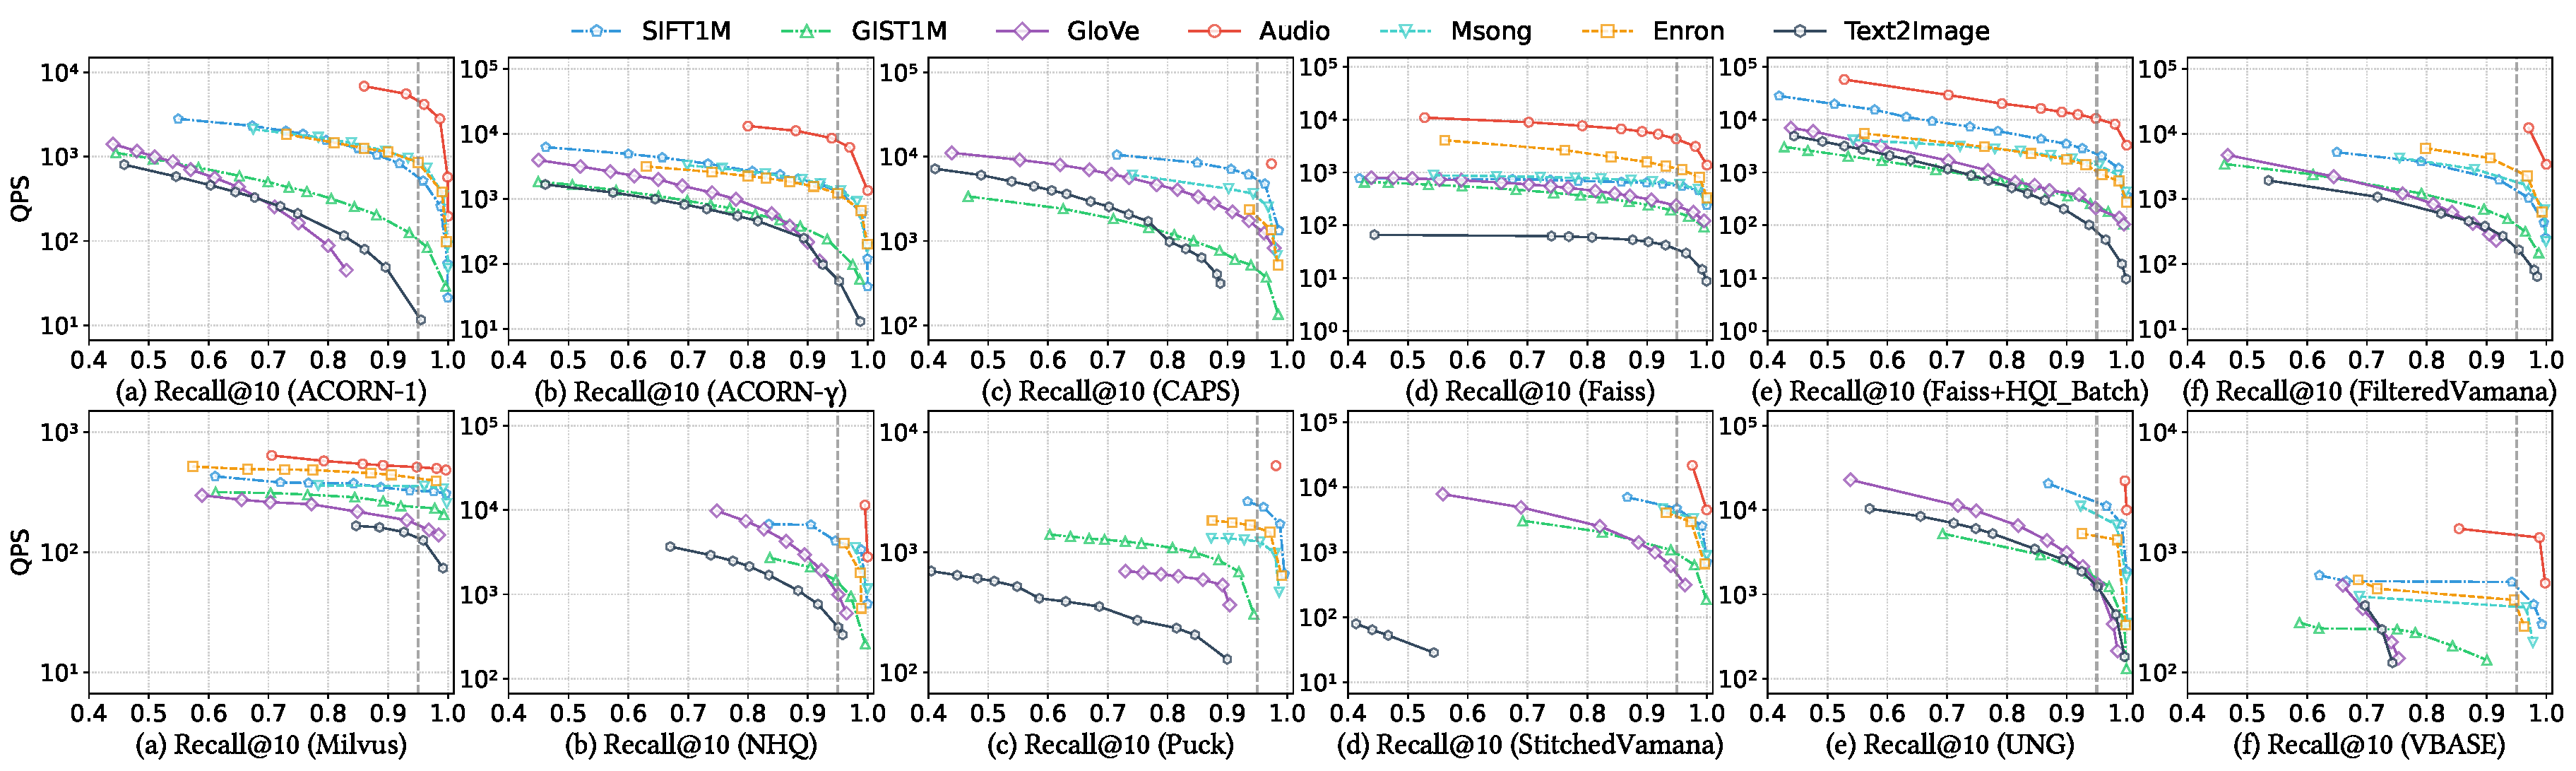
\includegraphics[width=0.95\textwidth]{figures/exp/exp_6_1.pdf}
%		\caption{Effect of Different Datasets on AF-ANN Search}
%		\label{fig:exp_6_1}
%	\end{figure*}
	
	%4.2.7
	
	% \begin{table}[t]
		% 	\centering
		% 	\setlength{\abovecaptionskip}{0.05cm}
		% 	\caption{Time and space overhead of range filtering index construction}
		
		% 	\label{tab:Range Filtered}
		% 	\resizebox{\columnwidth}{!}{
			% 		\begin{tabular}{l l c c c c c }
				% 			\toprule
				% 			\textbf{Dataset} & \textbf{Metric} & \textbf{DSG} & \textbf{iRange} & \textbf{SeRF} & \textbf{UNIFY} & \textbf{WinFilter} \\
				% 			\midrule
				% 			\multirow{3}{*}{DEEP} 
				% 			& Index time(s)  & 4156 & 1128 & \textbf{189.89} & 7510 & 32843 \\
				% 			& Index size(GB)  &  4.6 & 0.92 & \textbf{0.80} & 1.43 & 2.41  \\
				% 			& Peak memory(GB) &  7.78 & 3.54 & \textbf{1.38} & 2.61 & 7.08   \\
				% 			% \cmidrule{1-7}
				% 			\midrule
				% 			\multirow{3}{*}{YT-Audio} 
				% 			& Index time(s)   & 15314 & 1039 & \textbf{187.20} & 5905 & 30904    \\
				% 			& Index size(GB)    & 4.3 & \textbf{0.7} & 1.04 & 1.55 & 1.32  \\
				% 			& Peak memory(GB)   & 7.5 & 3.16 & \textbf{1.57} & 2.97 & 6.95  \\
				% 			\midrule
				% 			\multirow{3}{*}{WIT} 
				% 			& Index time(s)  & 29492 & 7068 & \textbf{828.12} & 28759 & 94909\\
				% 			& Index size(GB) &  4.2 & \textbf{1.5 }& 15.34 & 8.71 & 1.59  \\
				% 			& Peak memory(GB)  & 21.7 & \textbf{12.32} & 15.87 & 24.38 & 15.29\\
				% 			% \cmidrule{1-7}
				% 			\bottomrule
				% 		\end{tabular}
			% 	}
		% \end{table}
	
	%\textit{\textbf{Different Datasets.}}  
	%\sout{To evaluate the performance of various methods across different datasets, we conduct experiments on 7 datasets, including one dataset Text2Image for OOD queries. Our analysis focuses on performance variations concerning dataset size, LID, and vector dimensionality.
	
%ykw: 这段话看着有问题
	%As shown in Figure~\ref{fig:exp_6_1}, all methods achieve their highest QPS and recall on Audio dataset. Because Audio has small scale, low dimensionality, and low LID. In contrast, all methods exhibit the lowest QPS and recall on the GIST1M and GloVe dataset besides the OOD dataset Text2Image. Because these two datasets have the largest scale and highest LID.
	
	%SIFT1M and Msong are similar datasets, with the key difference being that SIFT1M has lower dimensionality. The 4 algorithms (ACORN, Faiss, PASE, and NHQ) perform similarly on these two datasets, suggesting strong robustness to high dimensional datasets. In contrast, the remaining algorithms exhibit degraded performance on Msong, revealing a lack of adaptability to high dimensional datasets.
	
	%Most algorithms struggle to achieve high recall on GloVe, because it has the highest LID. Compare to other algorithms, the 4 algorithms (UNG, Faiss, CAPS, and Milvus) manage to maintain relatively high recall, demonstrating better adaptability to complex datasets. Notably, although vanilla Faiss performs worse on SIFT1M compared to Enron dataset, Faiss+HQI\_Batch outperforms on SIFT1M. Because batch optimization in HQI reduces query overhead and increases throughput.	}
	
	%\textcolor{green}{Most algorithms exhibit the worst performance on the OOD dataset Text2Image. However, ACORN, UNG, and FilteredVamana show relatively stable performance on Text2Image. Their performance drops less compared to in-distribution (ID) datasets such as GIST1M and GloVe, indicating better adaptability to OOD queries.}
	
\begin{figure*}[t]
	\centering
	
	% 1. 全局图例 (Legend) - 位置保持不变
	
\includegraphics[width=0.9\textwidth]{figures/exp/attribute_legend.pdf}
	
	% --- 主要改动:将以下三个 subfigure 全部放在同一行 ---
	
	% 2. 第一部分:两张图,共用标题
	% [b]表示按底部对齐,在一行内通常比顶部对齐[t]效果好
	% 宽度从\textwidth缩小到0.32\textwidth
	\begin{subfigure}[b]{0.39\textwidth}
		\centering
		% 内部图片宽度使用\linewidth,它会自适应为容器宽度(0.32\textwidth)
		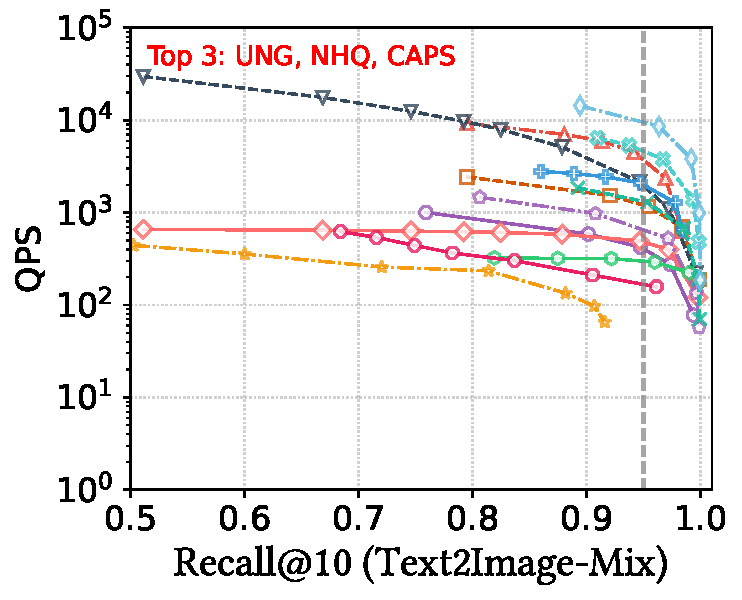
\includegraphics[width=0.495\linewidth]{figures/exp/attribute_multimodel.pdf}
		\hfill 
		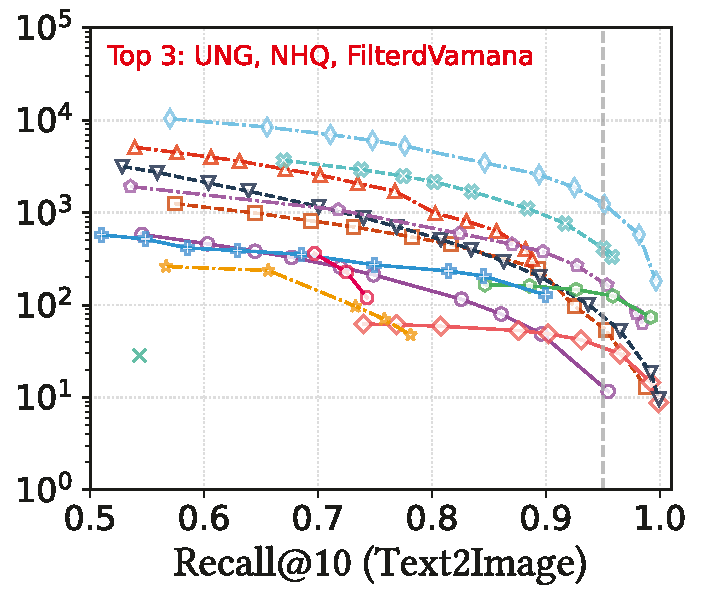
\includegraphics[width=0.47\linewidth]{figures/exp/attribute_multimodel_1.pdf}
		\caption{Multi-Modal}
		\label{fig:attribute-multimodal} 
	\end{subfigure}
	\hfill % 在第一部分和第二部分之间添加弹性间距
	% 3. 第二部分:两张图,共用标题
	\begin{subfigure}[b]{0.39\textwidth}
		\centering
		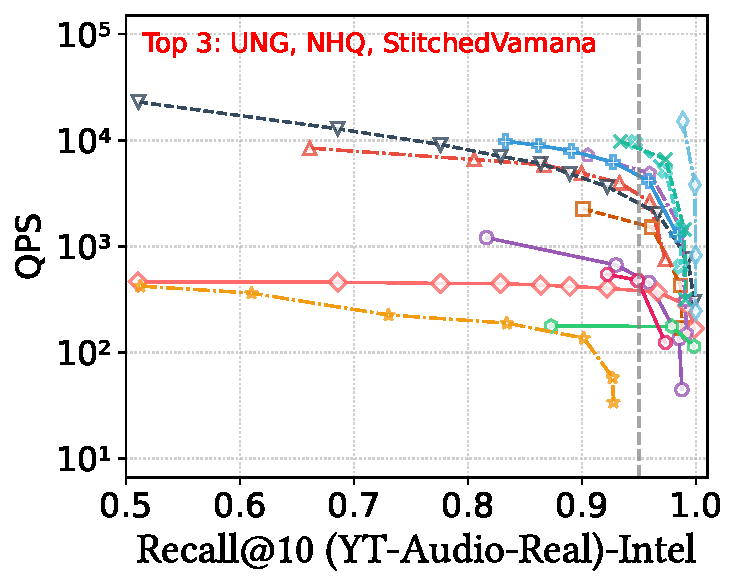
\includegraphics[width=0.495\linewidth]{figures/exp/attribute_85.pdf}
		\hfill
		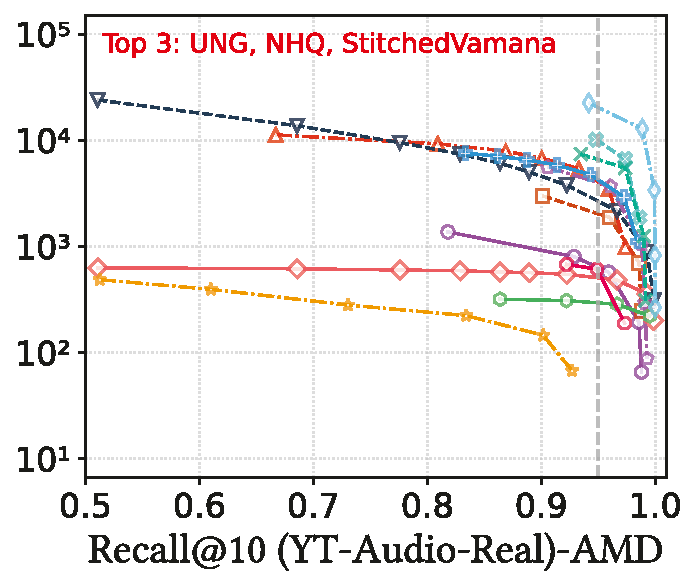
\includegraphics[width=0.47\linewidth]{figures/exp/attribute_71.pdf}
		\caption{Cross-Platform}
		\label{fig:attribute-cross-platform}
	\end{subfigure}
	\hfill % 在第二部分和第三部分之间添加弹性间距
	% 4. 第三部分:只有一张图
	\begin{subfigure}[b]{0.203\textwidth}
		\centering
		% !!! 注意:这是一个占位符,请替换成您自己的第五张图 !!!
		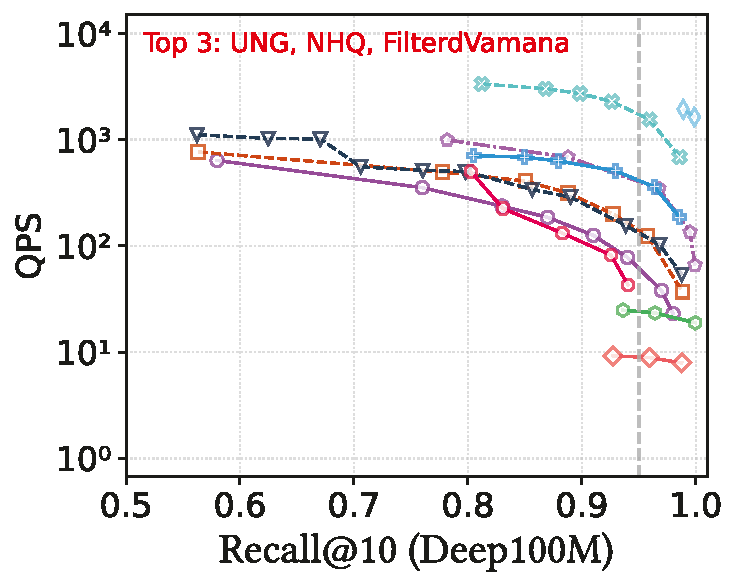
\includegraphics[width=0.96\linewidth]{figures/exp/attribute_100M.pdf} 
		\caption{Big Dataset}
		\label{fig:attribute big dataset}
	\end{subfigure}
	
	% 5. 全局总标题
	\caption{\textcolor{violet}Scalability Study——Attribute}
	\label{fig:TrinityExtension——Attribution_main}
\end{figure*}
	
%	\subsubsection{Scalability Study}
	\textit{\textbf{\textcolor{blue}{Multi-Modal Queries.}}} \textcolor{blue}{
		We conduct experiments on the text2image-mix dataset. This dataset contains image and text vectors and is a hybrid multimodal dataset. As shown in Figure~\ref{fig:attribute-multimodal}, UNG and NHQ consistently perform best, followed by CAPS.
		Although this dataset mixes two modalities, the vector space distributions of different modalities often differ significantly. In practice, this means that the experiments effectively treat the image and text subsets as separate datasets, since the ground truths for each query belong to the same modality. Therefore, the performance on this dataset is similar to the results shown in Figure~\ref{fig:exp_1_1_SingleLabel_1thread}.
		In contrast, the text2image dataset shown in Figure~\ref{fig:attribute-multimodal} is different. The query set and the base dataset belong to two completely different modalities. Queries are far from the dataset points, and the ground truths are more dispersed and not clustered together. To find the ground truths, algorithms typically need to examine more points, which leads to degraded performance.
		%	We conduct experiments on the text2image-mix dataset. This dataset contains both image and text vectors. It is a more complex multimodal dataset. As shown in Figure~\ref{fig:attribute-multimodal}, although the queries are more complex, UNG and NHQ still perform the best. CAPS is the next best.
		%	Since the dataset mixes two modalities, the ground truth of the query set usually corresponds to the same modality. The nearest neighbors in the index are often from the same modality because they are closer in distance. Therefore, the search results on this dataset are similar to those in Figure~\ref{fig:exp_1_1_SingleLabel_1thread}. UNG and NHQ perform the best. CAPS clusters based on vector similarity. It actually clusters the vectors into the same modality. Then it uses attribute filtering to divide the data further. This allows CAPS to quickly find nearest neighbors that meet the filter conditions.
		%	In contrast, the text2image dataset shown in Figure~\ref{fig:exp_6_1} is different. The queries and the dataset are from different modalities. The queries are far from the dataset. The ground truths are also scattered and not clustered together. To find the ground truths, the algorithm often needs to traverse more points. This is a greater challenge for the algorithms.
		%	We conducted extensive scalability experiments on the Text2Image-Mix dataset. This dataset contains both image and text vectors. It represents a more complex multimodal query scenario. As shown in Figure 12, the UNG and NHQ algorithms still achieve the best performance, followed closely by CAPS.
		%	In the Text2Image-Mix dataset, the ground truth of the query vector is usually the corresponding vector in the same modality. Since the neighbor relationships in the graph are often based on vector distance, vectors of similar modalities naturally form closer connections in the graph. Therefore, during the search process, the algorithm tends to traverse efficiently within the same modality. This makes the search mechanism similar to our experiments on single-modality datasets, thus maintaining high performance.
		%	The good performance of the CAPS algorithm is due to its unique hierarchical space partitioning strategy. It first clusters vectors based on similarity. In multimodal data, this clustering naturally groups vectors of similar modalities into the same cluster. Then, CAPS further partitions these clusters using attributes. This allows it to quickly find the nearest neighbors that meet the filtering conditions.
		%	It is worth noting that, compared to the OOD dataset discussed in the "Dataset Impact" section, the Text2Image-Mix dataset also involves modality differences. However, its complexity lies in modality mixing. The OOD dataset, on the other hand, has a modality gap. This often requires traversing a broader and more sparse search space to find the ground truth. It poses a more severe challenge to the algorithm.
	}
	
	\textit{\textbf{\textcolor{blue}{Different Hardware Environments.}}} 
%	\textcolor{cyan}{To investigate the impact of different server configurations on the performance of the algorithms, we conducted additional experiments on Server B using the YT-Audio-Real dataset, and the results are shown in Figure~\ref{fig:Different Computer}. Compared with the experimental results on Server A shown in Figure~\ref{fig:exp_1_1_SingleLabel_1thread}f, the relative ranking of the algorithms remains largely unchanged, indicating that the performance of these methods is not significantly affected by differences in CPU configurations. Due to the lower CPU frequency and smaller RAM capacity of Server B compared to Server A, the QPS values are slightly lower across all methods.}
	\textcolor{red}{To investigate the impact of different server configurations on the performance of the algorithms, we conduct additional experiments on an Ubuntu 20.04 server equipped with dual Intel(R) Xeon(R) Gold 6330 CPUs @ 2.00GHz featuring 128GB of RAM and 84 MiB of L3 cache using the YT-Audio-Real dataset, and the results are shown in Figure~\ref{fig:attribute-cross-platform}. It is not difficult to see that the relative ranking of the algorithms under the two servers essentially remains unchanged, indicating that the performance of these methods is not significantly affected by differences in CPU configurations. Due to the lower CPU frequency, reduced RAM capacity, and smaller L3 cache, all methods demonstrate slightly lower QPS values.}

	\textit{\textbf{\textcolor{blue}{Large-scale Datasets.}}} 
	\textcolor{violet}{As shown in the Figure~\ref{fig:attribute big dataset}, on the 100M dataset, UNG and NHQ still exhibit excellent performance, demonstrating good adaptability to large-scale datasets. However, this also comes with significant memory overhead. The clustering-based algorithm Faiss+HQI\_Batch shows moderate performance but has very low memory overhead, which also has certain practical significance. Furthermore, we do not present the results of StitchedVamana and CAPS, as their recall remained consistently low. StitchedVamana sets the search entry point to 0 by default, which makes it prone to getting stuck in local optima when the entry is far from the target region, hindering effective navigation. CAPS, on the other hand, is limited by its implementation and achieves a recall of only around 0.2.}
%		we do not present the experimental results for StitchedVamana because its recall consistently remains at a very low level. This is due to its search starting point being set to 0 by default, when the entry point is far from the target area, it easily gets stuck in a local optimum, making it difficult to navigate to the vicinity of the correct point.}
	
	
	
%	\textit{\textbf{Multimodel, 85 and Deep100M.}} \textcolor{red}{The fig is Figure \ref{fig:TrinityExtension——Attribution}}
	
% 使用 figure* 环境来实现图片横跨双栏
% 使用 figure* 环境来实现图片横跨双栏


	\begin{figure}[t]
		\centering
		
		
		\hspace*{5pt}
		% 放大的图例(占满单栏)
		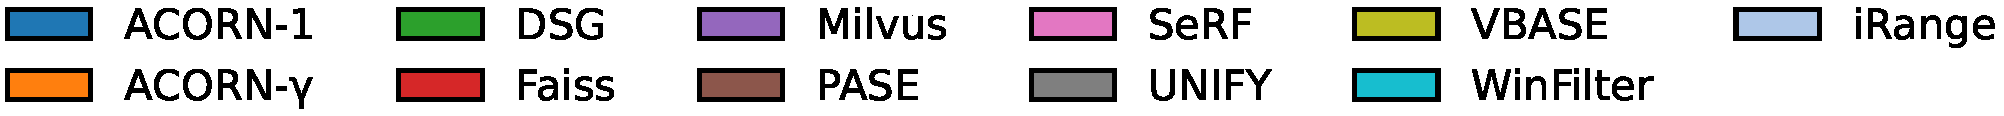
\includegraphics[width=0.98\columnwidth]{figures/indexData/rangeFilter_legend_only.pdf}
		
		%\vspace{0.1cm}
		
		% 三图横排
		\begin{subfigure}[t]{0.495\columnwidth}
			\centering
			\captionsetup{font=small}
			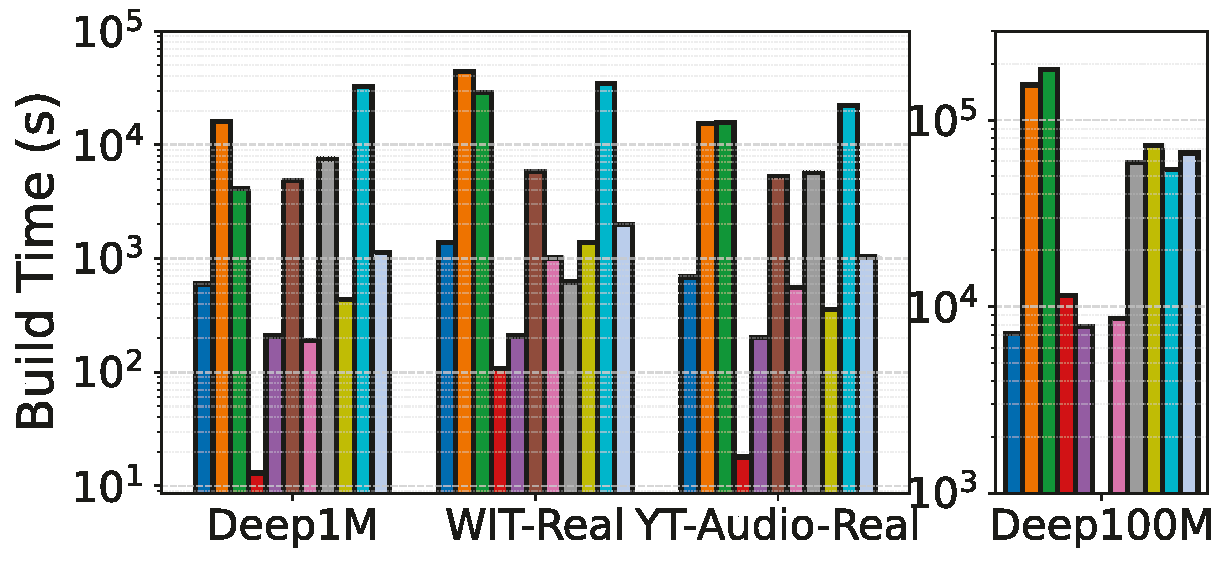
\includegraphics[width=\linewidth]{figures/indexData/rangeFilter_build_time_comparison_query.pdf}
			\caption{\footnotesize Construction Time}
			\label{fig:rangeFilter_build_time}
		\end{subfigure}
		\hfill
		\begin{subfigure}[t]{0.495\columnwidth}
			\centering
			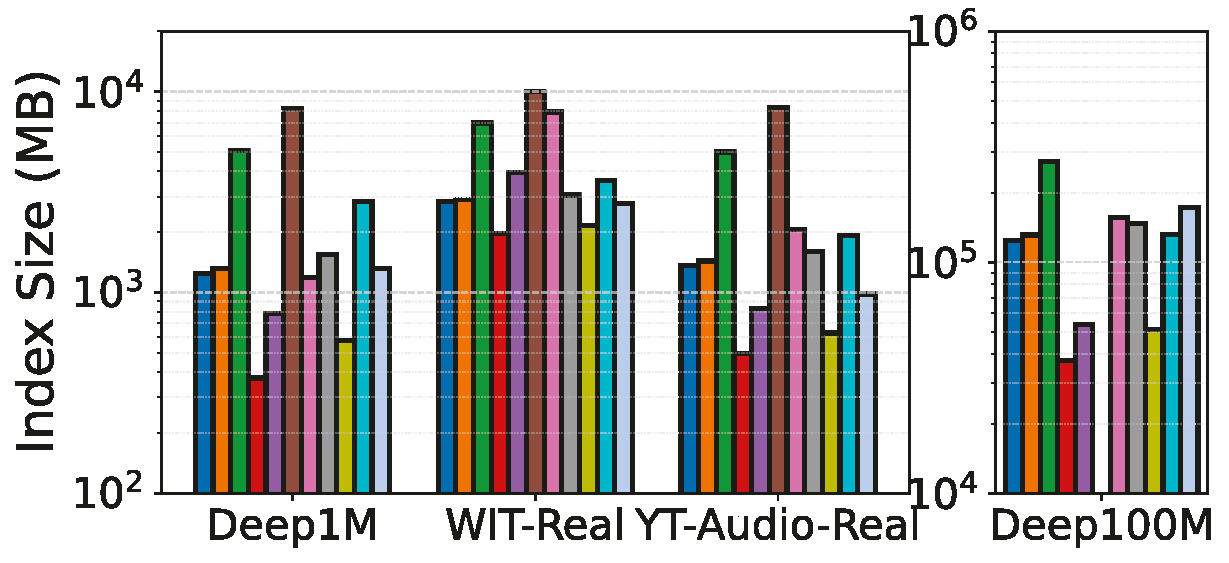
\includegraphics[width=\linewidth]{figures/indexData/rangeFilter_index_size_mb_comparison_query.pdf}
			\caption{\footnotesize Index Size}
			\label{fig:rangeFilter_index_size_mb}
		\end{subfigure}
		\hfill
		\begin{subfigure}[t]{0.495\columnwidth}
			\centering
			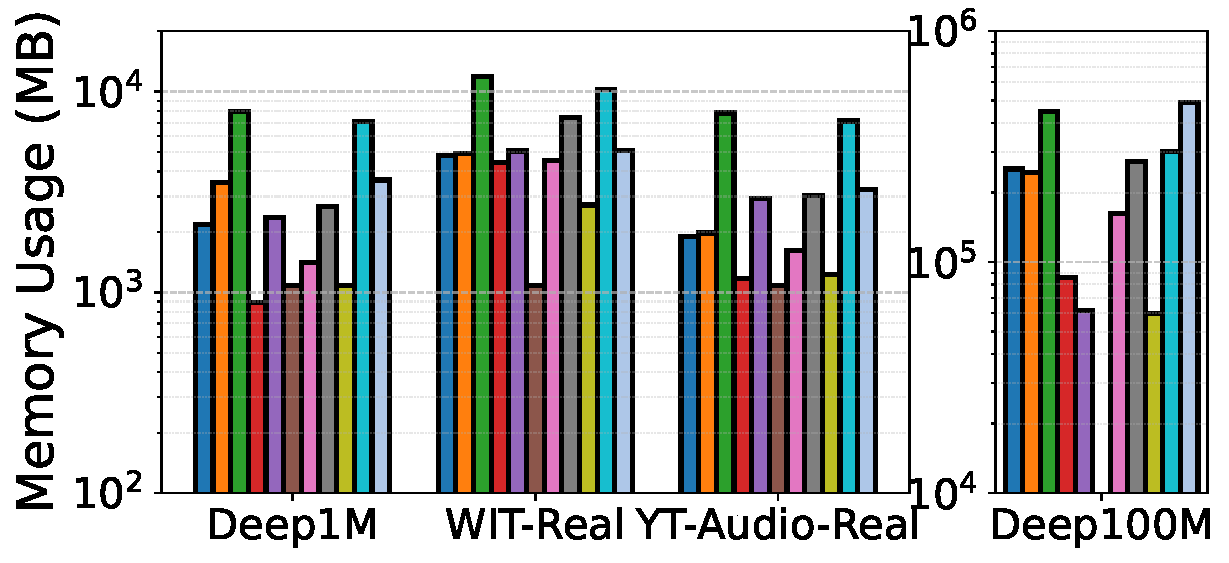
\includegraphics[width=\linewidth]{figures/indexData/rangeFilter_memory_mb_comparison_query.pdf}
			\caption{\footnotesize Build Peak Memory}
			\label{fig:rangeFilter_build_memory_mb}
		\end{subfigure}
		\hfill
		\begin{subfigure}[t]{0.495\columnwidth}
			\centering
			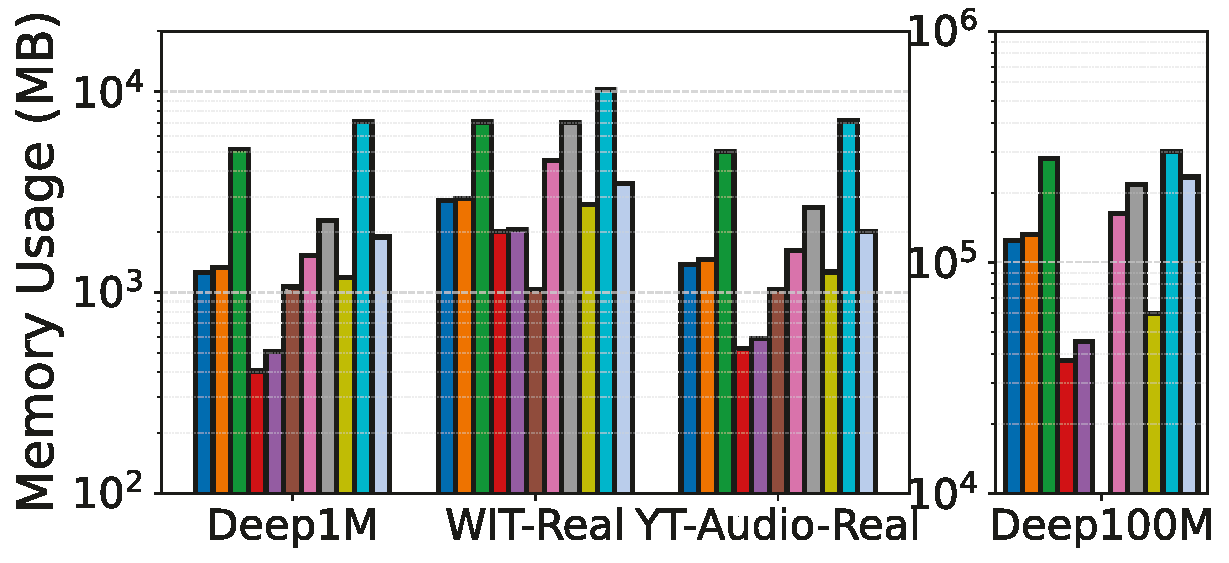
\includegraphics[width=\linewidth]{figures/searchMem/range_memory_comparison.pdf}
			\caption{\footnotesize Search Peak Memory}
			\label{fig:rangeFilter_search_memory_mb}
		\end{subfigure}
		
		%		\caption{Time and space overhead of range filtering index construction}
%		\caption{Time and space overhead of index construction}
		\caption{\textcolor{violet}{Time and Space Overhead}}
		\label{fig:rangeFilter_build_index_comparison}
	\end{figure}
	\subsection{Range Filtering}
	\textcolor{blue}{Due to the limitations of existing range filtering algorithms, our experiment uses only a single attribute, with the dataset sorted in ascending order by value. The WIT-Real and YT-Audio-Real datasets use real attribute values, while the rest use randomly generated ones. }
	\subsubsection{\textcolor{violet}{Time and Space overhead.}}
	
	%Similar to the evaluation of \textit{Attribute Filtering} algorithms, 
	Similarly, we also evaluate \textcolor{orange}{4} key metrics mentioned above in \textit{Range Filtering} algorithms. \textcolor{orange}{Note: For regular-scale datasets, all algorithms build indexes using a single thread. For the large-scale dataset Deep100M, all algorithms use 64 threads for index construction to improve efficiency, except DSG, which only supports single-threaded construction.}
	
	\textit{\textbf{Index construction time.}}
%	As shown in the Figure~\ref{fig:rangeFilter_build_time}, for regular-scale datasets, Faiss builds the index fastest. As Faiss obtains subsamples through sampling and calculates the cluster centroid, the computational complexity is significantly reduced.
%
%	WinFilter and ACORN-\(\gamma\) take the longest.
%	WinFilter relies on a tree structure, requiring separate nearest-neighbor graphs per node. This causes redundant computation and high costs, especially for large datasets.
%	ACORN-\(\gamma\) expands the neighbor list of each node to provide more candidate paths, which increases both computation and storage costs. It also prunes distant neighbors to save storage space. However, this introduces additional overhead and slows down the construction process.
%	
%	\textcolor{orange}{On large-scale datasets, ACORN-1 achieves the fastest index construction, primarily due to its similarity to the original HNSW construction process and its use of fewer candidate neighbors in the upper layers. SeRF, another HNSW-based method, also exhibits very short construction time by losslessly compressing multiple HNSW graphs into a unified structure and accelerating the process through dynamic pruning and skip-connection optimizations.
%	As two methods both based on IVF\_Flat, Milvus and Faiss achieve short indexing times. Milvus is even faster, mainly due to its cache-aware optimization, which significantly reduces CPU cache misses.}
%	\textcolor{orange}{
%	DSG only supports single-threaded construction, resulting in the longest build time.}
	\textcolor{orange}{
	As shown in Figure~\ref{fig:rangeFilter_build_time}, Faiss, based on the IVF\_Flat architecture, achieves fast index construction through subset sampling and centroid computation, which lowers the computational cost. 
	As another IVF\_Flat-based method, Milvus performs even better on large-scale datasets, mainly due to its cache-aware optimization that greatly reduces CPU cache misses.}
	
		\textcolor{orange}{
	ACORN-1 also achieves highly efficient index construction, especially on large-scale datasets. This efficiency stems from its construction process, which closely resembles that of the original HNSW, and from reducing the number of candidate neighbors in the upper layers, thereby lowering computational cost. SeRF, another HNSW-based method, also exhibits very short construction time. During construction, it attaches timestamp information to edges, keeping the total time comparable to building a single HNSW graph, which enables efficient construction even on large datasets.}
	
		\textcolor{orange}{
	In contrast, WinFilter relies on a tree-based structure, where a separate nearest neighbor graph must be built for each node. This design introduces redundant computation and high construction cost. However, on large-scale datasets, the preprocessing phase of WinFilter was replaced with a base algorithm in the experiments, thus avoiding significant time overhead.}
	
		\textcolor{orange}{
	ACORN-\(\gamma\)  extends the neighbor list of each node to provide more candidate paths, which increases both computational and memory overhead. Although it prunes distant neighbors to save storage, the additional construction logic still incurs substantial time cost.}
	
%	The reason for the high construction time of ACORN-$\gamma$ has been explained in the attribute filtering section and is therefore omitted here.
	
		\textcolor{orange}{
	DSG is an optimization over SeRF, incorporating a rectangular tree structure for index management. This makes the construction process more complex and costly. In addition, on Deep100M, DSG uses single-threaded construction, resulting in the longest build time.}
	
	\textit{\textbf{Index size.}} 
	As shown in Figure~\ref{fig:rangeFilter_index_size_mb}, Among all algorithms, Faiss has the smallest index size. Because IVF only adds centroid data and partition information to the vector dataset, the IVF index is only slightly larger than the vector dataset.

	
	PASE requires the most storage. Its implementation likely wastes space due to alignment padding and inefficient encoding. %(e.g., Base64).
	\textcolor{orange}{Additionally, DSG also results in a large index size, especially on large-scale datasets. As an enhancement over SeRF, DSG stores additional metadata for each edge in its index structure. While this design improves retrieval accuracy, it significantly increases the index size on massive datasets.}
%	\textcolor{orange}{DSG is an improvement over SeRF. Compared to SeRF, DSG stores additional information for each edge in its index structure, resulting in a significant increase in index size on large-scale datasets.
%	}
	
	%SeRF maintains a compact index for low-dimensional data. However, for high-dimensional dataset (WIT), SeRF stores more edges and dynamic range data, significantly increasing its size.
	
	\textit{\textbf{Build peak memory.}}  
	\textcolor{orange}{As explained in the attribute filtering analysis, algorithms with larger index sizes (including the dataset) tend to exhibit higher build peak memory consumption. As shown in Figure~\ref{fig:rangeFilter_build_memory_mb}, range filtering also adheres to this pattern, while PASE deviates due to reasons discussed earlier.}  
	
	\textcolor{orange}{WinFilter also presents an exception:  its peak memory usage is also affected by the level of parallelism. Although the final index size remains relatively small, the peak memory usage increases significantly during both construction and search. During construction, this is caused by the parallel building of local indices for each tree node, which results in substantial temporary memory usage. Similarly, during search, WinFilter needs to load multiple local indices in parallel for different tree nodes, further contributing to high peak memory consumption.}
	

	
%	As Figure~\ref{fig:rangeFilter_build_memory_mb} shows, Faiss uses the least memory on low-dimensional datasets. It stores minimal temporary data during index construction.
%	
%	On low-dimensional datasets, DSG and WinFilter exhibit higher peak memory usage compared to other algorithms. This suggests that their index structures suffer from severe structural redundancy and are difficult to compress in low-dimensional scenarios.
%	
%	For high-dimensional dataset WIT, iRange achieves the lowest peak memory usage. It pre-builds graphs only for a limited number of intervals, avoiding explicit index construction for all possible query ranges. Its index structure remains stable in high dimensions without significant graph growth. This effectively controls index size, making iRange more advantageous for high-dimensional datasets.
%	In contrast, \textcolor{orange}{Milvus exhibits the highest memory consumption,}


		\textit{\textbf{\textcolor{orange}{Search peak memory.}}}  
		\textcolor{orange}{As shown in Figure~\ref{fig:rangeFilter_search_memory_mb}, the peak memory usage during search generally follows a similar trend to that observed during index construction. This observation is consistent with our earlier analysis in the attribute filtering section.}
		
	\begin{figure*}[t]
		
		\centering
		
		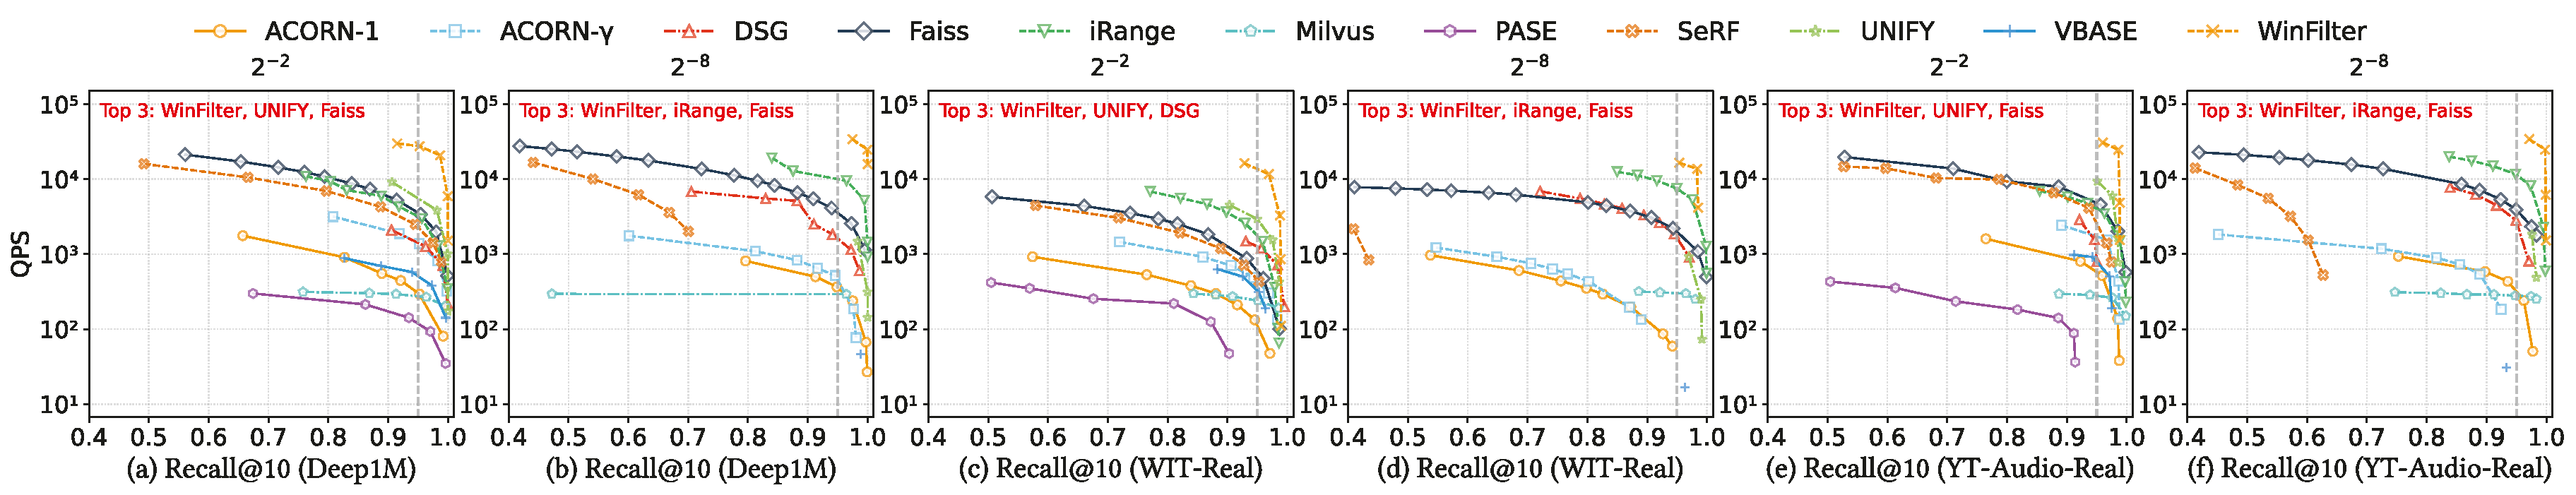
\includegraphics[width=0.92\textwidth]{figures/exp/exp_8_2.pdf}
		\caption{Performance of RF-ANN Search}
		\label{fig:exp_8_2}
	\end{figure*}
	
	
	\subsubsection{Performance Evaluation. }
	
	In this experiment, we follow the query range definition adopted by prior work~\cite{HQI}. \textcolor{red}{Specifically, for a given query, the range ratio is defined as $2^{-i}$	when the query range covers $\frac{n}{2^i}$ data points, where $n$ is the total dataset size.}
	% Based on this definition, we evaluate algorithm performance under 4 query range settings: $2^{-2}$, $2^{-4}$, $2^{-6}$, and $2^{-8}$. \textcolor{blue}{Due to the limitations of existing range filtering algorithms, the range filtering experiment only uses one attribute, and the dataset is sorted in ascending order according to the attribute value size. WIT-Real and YT-Audio-Real use real attribute values, and the rest use randomly generated attribute values.}
	%\textcolor{red}{Some algorithms don't support using actual attributes as search keys, instead requiring an ID (the primary key, ranging from $0$ to $n-1$). Therefore, we uniformly use this ID as the search key. This ID is pre-sorted according to its corresponding real attribute, allowing us to map an attribute to its ID without loss of generality for efficient range queries.} 
	Based on this definition, we evaluate algorithm performance under four query range settings: $2^{-2}$, $2^{-4}$, $2^{-6}$, and $2^{-8}$. For space considerations, Figure~\ref{fig:exp_8_2} reports results for only the largest ($2^{-2}$) and smallest ($2^{-8}$) range ratios. The experimental results show consistent performance across all datasets and query ranges.
	
	%Due to space constraints, Figure~\ref{fig:exp_8_2} reports results for only the largest ($2^{-2}$) and smallest ($2^{-8}$) range ratios. The experimental results show that across all datasets (YT-Audio-Real, WIT-Real, and Deep1M) and query ranges.
	
	\textcolor{blue}{
	WinFilter maintains optimal performance by building an index for each tree node. It then performs an ANN search on the relevant nodes and post-filters the results, ensuring high recall and QPS.
	In contrast, iRange dynamically constructs a search graph during query time. This method has low overhead and performs well in small-range queries, but its performance degrades as the query range increases.
	UNIFY utilizes a skip list for localization followed by a linear scan for searching in small-range query scenarios. Its performance is generally lower than graph-based structures like iRange in these cases.
	Interestingly, Faiss, aided by its efficient ID selector for filtering, calculates distances for only a small subset of points in small-range scenarios. Consequently, it can outperform algorithms specifically designed for range searches.
	}
%	WinFilter consistently delivers the best performance. This highlights its robustnes, which performs ANN search over only relevant tree nodes and merges results efficiently, making it highly effective for static range query scenarios.
%	
%	iRange offers a good balance between query efficiency and recall, demonstrating stable performance across both datasets and range sizes. In contrast, UNIFY experiences a notable drop in performance under narrow query ranges, suggesting that its HSIG structure—despite incorporating skip lists for pre-filtering—still has limitations in such scenarios. However, by leveraging HNSW and bitmap-based post-filtering, UNIFY performs competitively under broader range conditions, demonstrating strong scalability.
	
%	SeRF exhibits relatively weak overall performance, with a significant drop in recall under small-range query scenarios. This suggests that while its compressed graph structure is space-efficient, it has a substantial negative impact on query performance.

	\textcolor{blue}{SeRF demonstrates relatively weak overall performance, with a pronounced drop in recall under small-range query scenarios. This is because SeRF compresses the entire HNSW graph by attaching range information to its edges. However, during small-range queries, its multi-filtering mechanism requires scanning a large number of edge entries that are irrelevant to the current query range, introducing fixed computational and memory access overhead. Additionally, graph traversal may lead to the exploration of numerous invalid neighbors, increasing the likelihood of the search becoming trapped in local optima and further degrading performance.
	}
	
	%	 修改此处
	ACORN performs similarly on both large and small range queries, but its overall performance is worse than the other methods. Unlike other range filtering algorithms, ACORN is not designed with specialized data structures  to achieve efficient range filtering. In fact, the graph structure used by ACORN for attribute filtering is the same as that used for range filtering.
	
%	For third-party library and databases, Figure~\ref{fig:exp_8_2} shows that Faiss performs well in range filtering and even outperforms some specialized range query algorithms in certain cases. 
%	%\textcolor{blue}{since attributes are pre-sorted in range filtering scenarios, the filtering overhead is minimal, leading to improved query performance. Similar to the selectivity observed in attribute filtering. }
%	Faiss performs better in small-range filtering scenarios because it searches over the filtered vectors. With a smaller range, fewer points remain after filtering, resulting in lower computational cost. In addition, the performance of Faiss is influenced by data dimensionality; the higher the dimensionality, the worse the performance.
	
	Vector databases  show relatively poor performance on range queries. Among them, Milvus performs more balanced across both small-range and large-range queries, even surpassing ACORN under high recall settings. PASE performs poorly on small-range queries, with recall lower than 0.1, due to its post-filtering strategy. 
	VBASE performs moderately; it works well for large-range queries, but for small-range queries, although it achieves high recall, its QPS is quite  low.
	
	
	
%	\sout{It is important to note that this range query experiment is conducted under a fully static setting. Under such conditions, UNIFY, iRange, SeRF, and WinFilter require the dataset to be sorted by attribute prior to index construction. In contrast, DSG  supports dynamic index construction with unordered attribute insertions, making it more suitable for streaming or incremental data scenarios. This flexibility highlights its superior extensibility in real-world applications.}
	
	%\subsubsection{Robustness.}
	
	
	%\begin{figure*}[htbp]
	%	\centering
	%	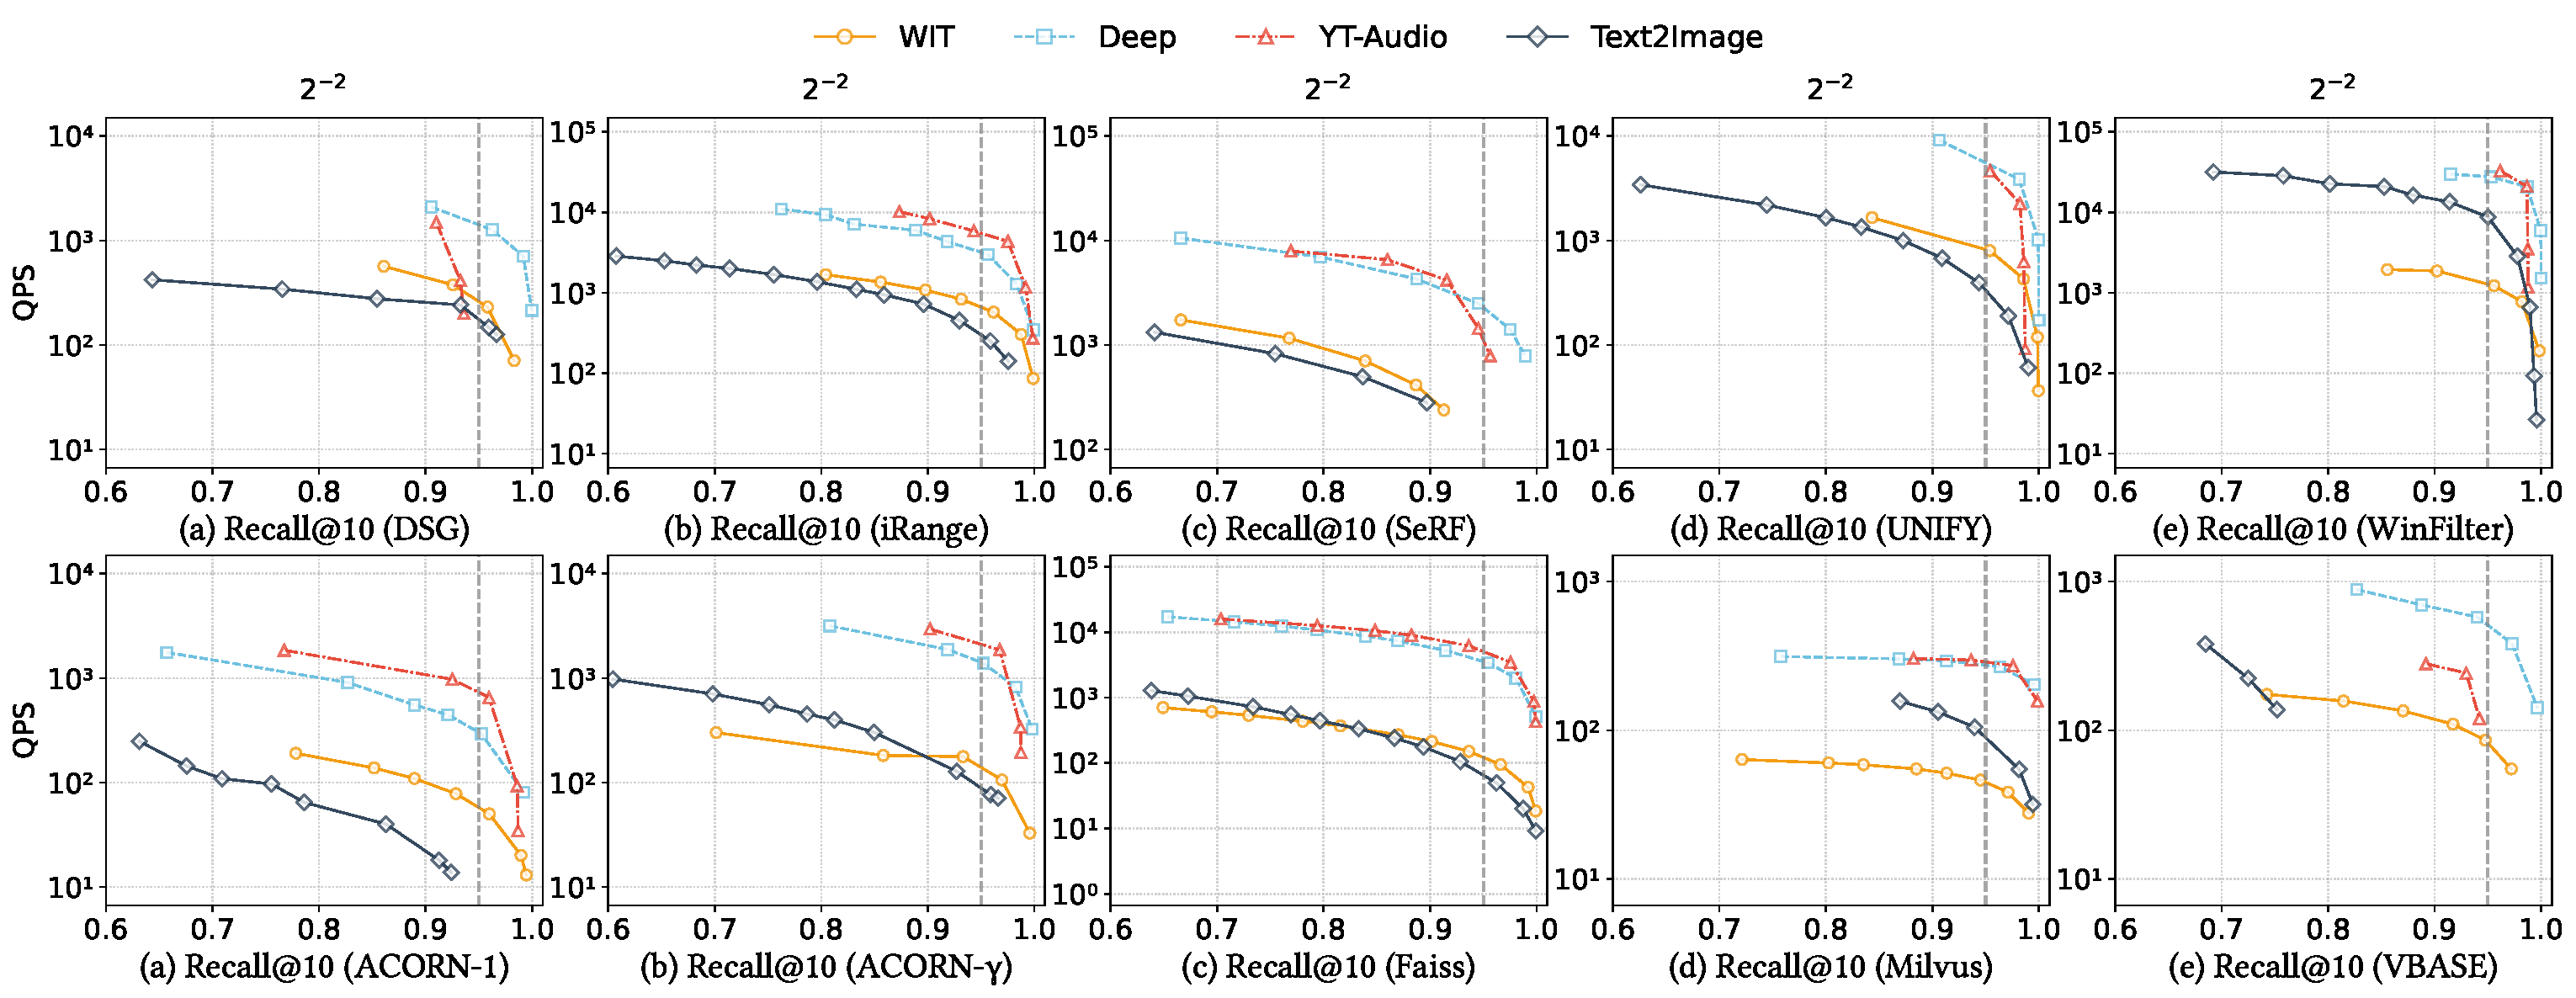
\includegraphics[width=0.80\textwidth]{figures/exp/exp_8_3.pdf}
	%	\caption{Effect of Different Datasets on RF-ANN Search}
	%	\label{fig:exp_8_3}
	%\end{figure*}
	
%	\textcolor{green}{To evaluate the robustness of the RF-ANNS algorithms in different scenarios, we add an OOD dataset in the experiments. As shown in Figure~\ref{fig:exp_8_3}, most methods perform worst on the Text2Image dataset. This is because OOD queries make the $k$-nearest neighbor distribution more sparse. As a result, the search needs to visit more nodes, which leads to an exponential growth in the search space and a sharp drop in efficiency.}
	
%	\sout{WinFilter shows the worst performance on the WIT dataset. This suggests that its performance is sensitive to the data dimensionality. ACORN has large performance differences across datasets, indicating weak robustness.
	
%	Among vector databases, Milvus performs well. VBASE is sensitive to datasets and achieved recall below 0.8 on Text2Image. PASE is excluded from this round of tests because it does not support datasets with dimensions over 512 and performed poorly in earlier experiments.
	
%	It is worth noting that most methods achieve similar performance on the Deep and YT-Audio datasets, which have similar LID values. This shows that RF-ANNS performance is largely affected by both the LID and the dimensionality of the dataset. A high LID and high dimensionality make hybrid queries more difficult.
	
%	However, even though Deep and YT-Audio have similar LID values, the DSG algorithm shows large performance differences between them. This means that DSG is more sensitive to changes in data distribution. }
	%	Its robustness is lower than that of other methods, possibly because it depends not only on LID but also on other complex data characteristics.
	%	To examine the robustness of RF-ANNS algorithms, we analyze their performance across different datasets. As shown in Figure~\ref{fig:exp_8_3}, the performance differences. All methods perform worst on WIT, which has the highest LID. On Deep and YT-Audio, which have similar LID, most algorithms achieve comparable performance. 
	%	This suggests that the effectiveness of RF-ANN search is mainly influenced by LID of the dataset. A higher LID inherently increases the difficulty of hybrid query.
	%	
	%	However, the DSG algorithm shows a noticeable performance gap between the Deep and YT-Audio datasets, despite their comparable LID. This indicates that DSG is less robust than other methods when facing dataset-dependent variations, possibly due to its sensitivity to data distribution beyond LID alone.
	
\begin{figure*}[t]
	\centering
	
	% 1. 全局图例 (Legend) - 位置保持不变
	
\includegraphics[width=0.9\textwidth]{figures/exp/range_legend.pdf}
	
	% --- 主要改动:将以下三个 subfigure 全部放在同一行 ---
	
	% 2. 第一部分:两张图,共用标题
	% [b]表示按底部对齐,在一行内通常比顶部对齐[t]效果好
	% 宽度从\textwidth缩小到0.32\textwidth
	\begin{subfigure}[b]{0.39\textwidth}
		\centering
		% 内部图片宽度使用\linewidth,它会自适应为容器宽度(0.32\textwidth)
		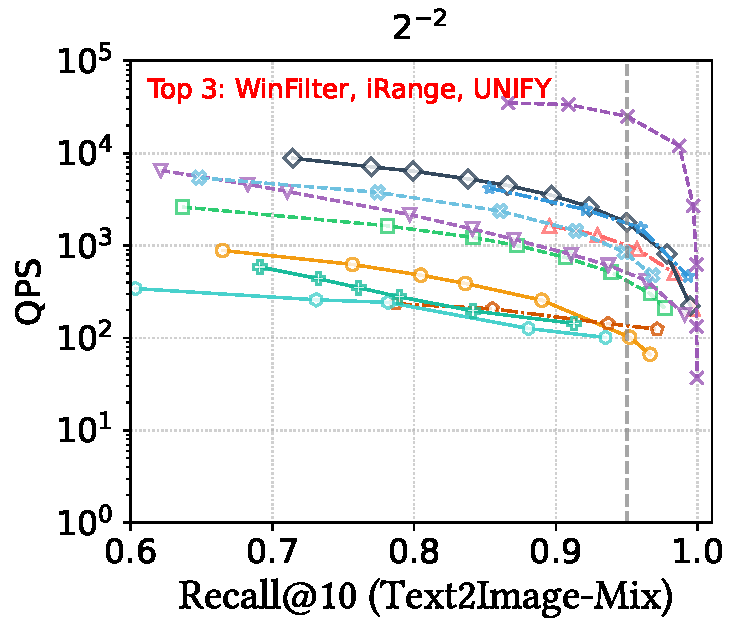
\includegraphics[width=0.495\linewidth]{figures/exp/range_multimodel.pdf}
		\hfill 
		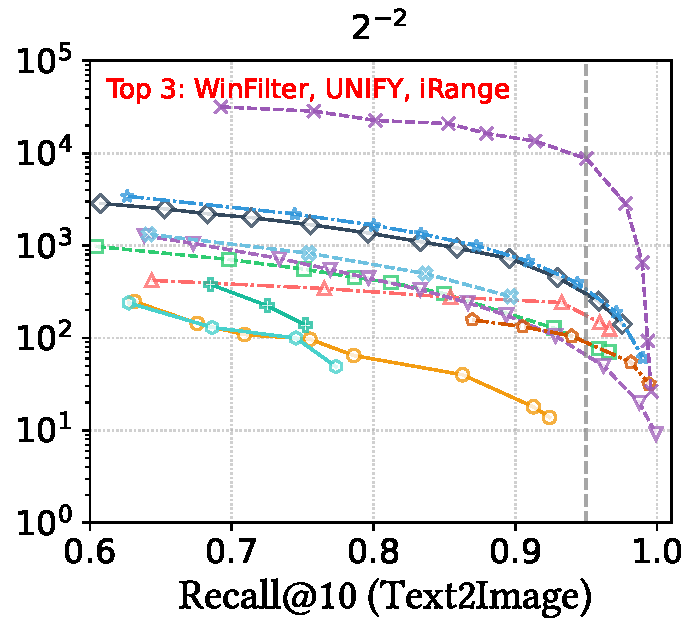
\includegraphics[width=0.47\linewidth]{figures/exp/range_multimodel_1.pdf}
		\caption{Multi-Modal}
		\label{fig:range-multimodal} 
	\end{subfigure}
	\hfill % 在第一部分和第二部分之间添加弹性间距
	% 3. 第二部分:两张图,共用标题
	\begin{subfigure}[b]{0.39\textwidth}
		\centering
		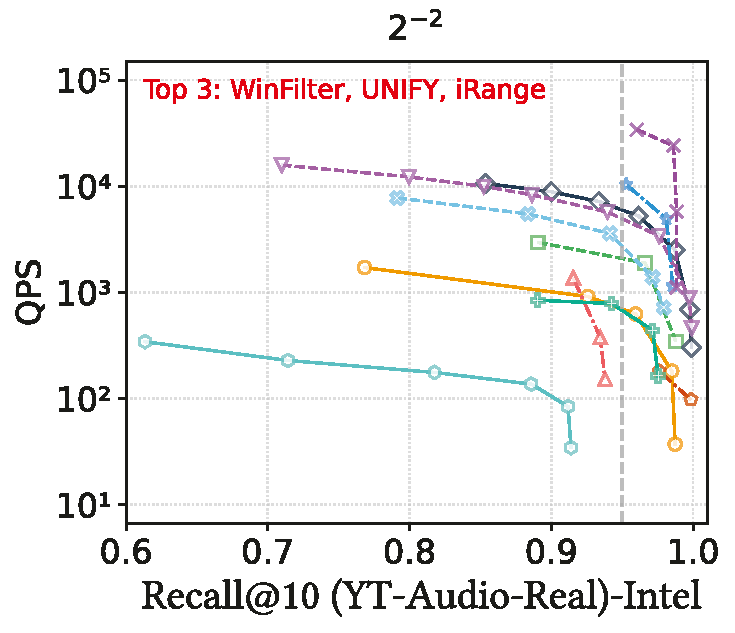
\includegraphics[width=0.495\linewidth]{figures/exp/range_85.pdf}
		\hfill
		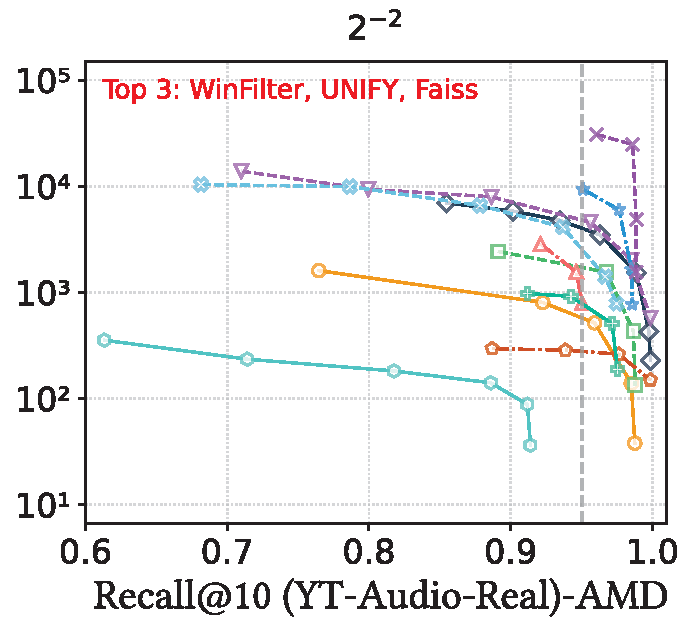
\includegraphics[width=0.47\linewidth]{figures/exp/range_71.pdf}
		\caption{Cross-Platform}
		\label{fig:range-cross-platform}
	\end{subfigure}
	\hfill % 在第二部分和第三部分之间添加弹性间距
	% 4. 第三部分:只有一张图
	\begin{subfigure}[b]{0.203\textwidth}
		\centering
		% !!! 注意:这是一个占位符,请替换成您自己的第五张图 !!!
		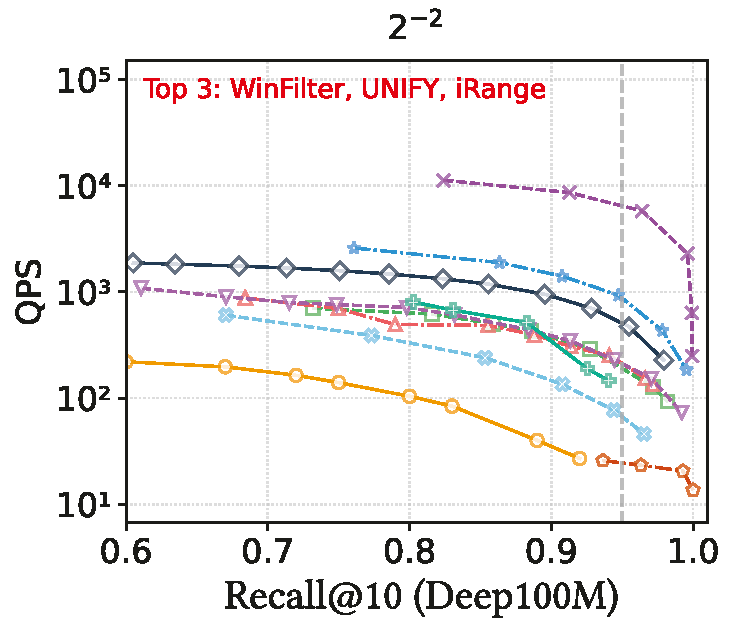
\includegraphics[width=0.96\linewidth]{figures/exp/range_deep100M.pdf} 
		\caption{Big Dataset}
		\label{fig: range big dataset}
	\end{subfigure}
	
	% 5. 全局总标题
	\caption{\textcolor{violet}Scalability Study——Range}
	\label{fig:TrinityExtension——Attribution_main}
\end{figure*}
	
	\subsubsection{Scalability Study}
	
	\textit{\textbf{\textcolor{blue}{Multi-Modal Queries.}}}
	\textcolor{blue}{
		Similar to attribute filtering, the performance of multimodal queries with range filtering shown in Figure~\ref{fig:range-multimodal} is also consistent with the single-modality results in Figure~\ref{fig:exp_8_2}. As shown in Figure~\ref{fig:exp_8_3}, the algorithms still perform the worst on multimodal datasets like Text2Image. This is because these range query algorithms are almost graph-based. Graph algorithms need more iterations to find true neighbors in OOD datasets.}
		
	\textit{\textbf{\textcolor{blue}{Different Hardware Environments.}}} 
	\textcolor{cyan}{Consistent with Section 4.2.4, we conduct additional range filtering experiments on the YT-Audio-Real dataset using the same server configuration, with results presented in Figure~\ref{fig:range-cross-platform}. Although the third-ranked algorithm differs, we consider the ranking order essentially unchanged since the performance of the third and fourth algorithms is comparable. So our findings remain consistent with those reported in Section 4.2.4. For brevity and due to space limitations, we omit further discussion of these redundant results.}
%	\textcolor{cyan}{Consistent with Section 4.2.4, we conducted additional range filtering experiments using the YT-Audio-Real dataset on the same server, with results shown in Figure \ref{fig:Different Computer range}. Compared with the original server's experimental results (Figure \ref{fig:exp_8_2}($e$)), the conclusions remain identical to those described in Section 4.2.4. Due to space constraints, these details are not reiterated here.}
	
	\textit{\textbf{\textcolor{red}{Large-scale Datasets.}}} \textcolor{red}{As shown in the figure~\ref{fig: range big dataset}, On the 100M dataset, the top 3 ranked algorithms (WinFilter, UNIFY, and iRange) remain unchanged. However, their high performance is achieved at the cost of extremely high memory consumption, as detailed in Figure~\ref{fig:rangeFilter_search_memory_mb}. Meanwhile, VBASE and Faiss demonstrate moderate performance but significantly lower memory consumption than the top three algorithms}.
	
	
%	\textit{\textbf{Multimodel, 85 and Deep100M.}} \textcolor{red}{The fig is Figure \ref{fig:TrinityExtension——Range}}
	\section{DISCUSSION}
	Based on the performance of the algorithms on different experimental scenarios, we discuss our findings as follows.
	
	
	\subsection{Recommendations.}
	%Based on the performance of different algorithms in experiments, we recommend algorithms suitable for different scenarios, as shown in the table \ref{tab:algo_scenarios}.
	
\begin{table*}[htbp]
	\caption{Algorithm Recommendation}
	\resizebox{\textwidth}{!}{
\begin{tabular}{|l|*{16}{c|}}
	\hline
	\multirow{2}{*}{\textbf{Application Scenarios / Algorithms}} 
	& \multicolumn{6}{c|}{\textbf{AF}} 
	& \multicolumn{5}{c|}{\textbf{RF}} 
	& \multicolumn{5}{c|}{\textbf{AF / RF}} \\
	\cline{2-17}
	& \textbf{NHQ} & \textbf{Filtered} & \textbf{Stitched} & \textbf{CAPS}  & \textbf{UNG} & \textbf{Puck} 
	& \textbf{DSG} & \textbf{iRange} & \textbf{SeRF} & \textbf{UNIFY} & \textbf{Win} 
	& \textbf{ACORN}& \textbf{Faiss} & \textbf{Milvus} & \textbf{VBASE} & \textbf{PASE} \\
	\hline
	\textbf{Query Performance} & S & M & S & M &\textbf{S} & S & M & M & W & M & S & M/M & M/M & M/M & W/W & W/W \\
	\textbf{Index Time} &M  &M  &M  &M  &M  &S  &W  &M  &S  &W  &W  &W/W &\textbf{S}/\textbf{S} &S/S  &W/M  &W/W  \\
	\textbf{Peak Memory} &W  &M  &M  &M  &M  &S  &W  &W  &M  &W  &W  &W/W  &\textbf{S}/\textbf{S}  &S/M  &S/M  &S/S \\
	\textbf{Large-Scale Dataset} & S & S & W & W &\textbf{S} &S  &M  &S  &M  &S  &\textbf{S}  &M/W  &W/M  &W/W  &M/M  &-  \\
	\textbf{Rare Attribute \& Low Range} &M  &M  &S  &S &\textbf{S}  &S  &S  &S  &W  &M  &\textbf{S} &M/M  &M/M  &W/W  &W/W  &W/W  \\
	\textbf{Robust to MultiModal Dataset} &S  &S  &W  &S  &\textbf{S}  &M  &M  &S  &M  &S  &\textbf{S}  &M/M  &W/M  &W/W  &W/W  &W/W  \\
%	\textbf{Robust to Attribute Distribution} &W  &W  &S  &S  &S  &S  &-  &-  &-  &-  &-  &S/-  &W/-  &\textbf{S}/-  &W/-  &W/-  \\
	\textbf{High LID Dataset} &S  &M  &S  &M  &\textbf{S}  &M  &M  &S  &M  &S  &\textbf{S}  &W/W  &M/S  &W/W  &W/M  &W/W  \\
	\textbf{General-Purpose} &\faCheck  &\faCheck  &\faTimes  &\faTimes  &\faCheck  &\faTimes  &\faTimes  &\faTimes &\faTimes  & \faCheck &\faCheck&\faTimes  &\faCheck  &\faCheck  &\faCheck&\faTimes  \\
	\hline
\end{tabular}
	}
	\vspace{1mm}
\begin{flushleft}
	\textbf{Performance Levels:} \quad \textbf{S} = Strongest, S = Strong, M = Medium, W = Weak, - = Not Supported \\
	\textbf{Recommendation:} \quad \faCheck = Recommended, \faTimes = Not Recommended
\end{flushleft}
	\centering

\end{table*}

	
	\subsubsection{\textbf{Attribute Filtering}}
%	We summarize the applicability of different algorithms across various attribute filtering scenarios in Table~\ref{tab:algo_scenarios}. Puck and UNG excel on large-scale datasets (S1). ACORN-1 and UNG achieve fast index construction (S2). UNG performs well on different datasets (S3, S4). In addition, CAPS performs well on hard datasets with high LID (S3), while NHQ and StitchedVamana perform better on easy datasets with low LID (S4).
%	Faiss and CAPS can generate relatively compact indexes with low memory usage, which is suitable for resource-constrained situations (S6). Milvus and Faiss serve as general-purpose solutions (S5). UNG stands out for its higher recall, precision, and QPS, and performs well in the OOD scenario (S7, S8).
\textcolor{orange}{
Overall, UNG, NHQ, and FilteredDisk\\-ANN demonstrate strong performance. However, UNG suffers from performance degradation when the attribute count differs between indexing and querying. NHQ, due to its distance fusion design, also experiences performance drops when there is a significant mismatch in attribute numbers between indexing and querying, and its performance is sensitive to attribute distribution. }

\textcolor{orange}{The two variants of FilteredDiskANN (FilteredVamana and StitchedVamana) support only single-attribute queries and multi-attribute OR queries. FilteredVamana supports dynamic insertion and disk-based indexing, making it suitable for memory-constrained scenarios. However, its disk-based construction significantly increases indexing time, and its performance is highly sensitive to attribute distribution. In contrast, StitchedVamana offers better search performance but performs poorly on 100M-scale datasets and OOD datasets.}

\textcolor{orange}{
CAPS, based on clustering, features low index space overhead. It offers flexible support for varying numbers of attributes and is optimized for low-selectivity attribute scenarios, but its overall performance is relatively moderate.
Puck is well-suited for large-scale datasets such as those with 100 million points. It offers fast index construction and low memory consumption in such scenarios. Moreover, it delivers high search performance in multi-threaded environments, making it an excellent choice for deployment on extremely large datasets.}


	\subsubsection{\textbf{Range Filtering}}
\textcolor{orange}{
	WinFilter achieves the best search performance but requires high time and memory resources during index construction. For large-scale datasets (e.g., with 100 million points), parameter tuning—particularly of tree height—is needed to prevent excessive index growth. When QPS and recall are not strict requirements, its basic variant, Vamana-WST, offers a more efficient alternative with significantly lower indexing overhead.
		}
	
	\textcolor{orange}{
	iRange has relatively low time and space costs for index construction; however, its search performance declines significantly with increasing query range. Despite offering threading parameters for indexing, it does not effectively utilize multi-core parallelism in practical scenarios.
	SeRF incurs low time and space overhead but achieves only moderate overall query performance, with notably weaker results in small-range query scenarios.
	DSG supports unordered dynamic insertions and range queries, but its index construction is limited to single-threaded execution, resulting in long build times and poor practical applicability.}
	
		\textcolor{orange}{
	UNIFY adopts multiple filtering strategies tailored to different query range sizes, avoiding the limitations of a single strategy in specific scenarios. It requires only one index to support all queries, allows dynamic insertions, and features low time and space overhead during index construction, making it a more general-purpose solution.}
%	Table~\ref{tab:algo_scenarios} also shows the application scenarios of range filtering. iRange performs well on large-scale datasets, combining efficient construction and excellent query capabilities (S1). Faiss performs well in fast index construction (S2). When processing hard datasets, WinFilter, iRange, and DSG are recommended (S3), while WinFilter and iRange also perform well on easy datasets (S4). For general applications, DSG supports dynamic updates, while UNIFY provides flexible filtering strategies (S5). Faiss and SeRF show superior memory efficiency (S6). For static queries with high recall, WinFilter is the best choice (S7). In addition, WinFilter also performs well in OOD scenarios (S8).

	\subsubsection{\textbf{General Algorithm}}
\textcolor{orange}{All of the following methods support both attribute filtering and range filtering.}

\textcolor{orange}{
ACORN demonstrates average overall performance. Among its variants, ACORN-1 shows significant advantages in indexing speed on billion-scale datasets, but suffers from high memory consumption and delivers only moderate performance.}

\textcolor{orange}{
Faiss, Milvus, and VBASE handle complex scenarios with advanced filtering operations more effectively. While they offer strong flexibility, their overall search performance is relatively modest. Relatively speaking, PASE performs less well across various aspects.}
	
	\subsection{Challenges}
	\subsubsection{\textbf{Attribute Filtering}}
	Most existing attribute filtering algorithms are graph-based, they typically outperform other methods in terms of query accuracy and efficiency. FilteredDiskANN leverages disk-based storage, making it more suitable for extremely large-scale datasets even in memory-constrained environments. Moreover, the index construction phase of graph-based algorithms is computationally intensive. Therefore, exploring GPU-based acceleration for graph construction and vector computation during indexing is promising. It can significantly improve the performance of graph-based methods.
	
	\textcolor{blue}{In addition, existing attribute filtering algorithms face two major limitations: strict requirements on attribute format and limited support for complex filtering conditions. }
%	For example, NHQ organizes attributes by column, which is suitable for uniformly structured data, but performs poorly in scenarios where the number of attributes varies across data points, resulting in poor scalability. Furthermore, NHQ only supports multi-attribute filtering with conjunctions ("AND" conditions). UNG is relatively more flexible in this regard, as it supports both "AND" and "OR" logic; however, it still cannot handle more complex Boolean expressions involving combinations of conjunctions and disjunctions.
%	In contrast, FilterDiskANN imposes no restrictions on the number of attributes per data point, offering better scalability. However, it currently supports only single-attribute filtering and disjunctions ("OR" conditions) across multiple attributes. Enhancing its capability to support more flexible Boolean combinations would effectively overcome the limitations of current approaches and significantly improve its practicality for diverse and complex query requirements.
%		}
		\textcolor{orange}{
For example, in multi-attribute scenarios, some algorithms only support Boolean OR logic (e.g., FilterDiskANN), while others only support Boolean AND logic (e.g., NHQ and CAPS). Although algorithms such as ACORN, UNG, and Puck support both AND and OR logic across multiple attributes, they still struggle to handle complex Boolean expressions that involve nested combinations of conjunctions (AND) and disjunctions (OR). In contrast, while databases and the vector search library Faiss support more expressive Boolean logic, their performance is often suboptimal in queries involving only basic attribute filtering.
Therefore, designing algorithms that can support complex filtering expressions while maintaining high query efficiency remains a key challenge to be addressed.
		}
		
	\textcolor{blue}{
	Besides, our research findings indicate that the distribution and selectivity of attributes significantly impact the performance of attribute filtering methods. Therefore, when designing algorithms, efforts should be made to minimize the coupling with specific attribute value distributions, in order to enhance the robustness and generalization ability of the algorithms under varying data conditions.}
	
%	Furthermore, current attribute filtering algorithms offer limited support for complex filtering conditions. For example, Filtered-DiskANN  supports single-attribute filtering, and in multi-attribute scenarios, it only supports OR conditions between attributes. 
%	%The original implementations of 
%	NHQ imposes strict constraints on the number of base and query attributes and only support AND conditions. While UNG is relatively flexible—supporting both AND and OR logic—it still lacks support for arbitrary Boolean expressions (e.g., combinations of AND and OR). The lack of flexible Boolean filtering remains a key challenge, limiting the practicality of hybrid query methods in real-world systems with diverse and complex query requirements.
	
	\subsubsection{\textbf{Range Filtering}}
	
	Except for DSG and UNIFY, most range filtering algorithms require the dataset to be pre-sorted before building the index. \textcolor{green}{Moreover, these methods do not support multi-attribute range queries. }Enhancing these methods to support an arbitrary number of range filterable attributes remains an open research challenge.
	
%	Our experiments show that graph compression methods often lead to poor query performance in RF-ANN search. To address this problem, subsequent algorithms usually optimize the index processing at the segment tree nodes. UNIFY newly proposes segment graphs and integrates multiple data structures to process queries. Although UNIFY performs slightly worse on small-range queries, its proposed index structure broadens the research direction.

\textcolor{blue}{
Experimental results show that different algorithms exhibit varying strengths under different query ranges. Therefore, designing a general range query algorithm that can adapt to diverse query conditions holds significant research value. For example, UNIFY demonstrates strong generality by dynamically selecting execution strategies based on the query range. Building on this idea, further exploration of more adaptive and high-performance range query algorithms is a promising direction for future research.}
	
		In our experiments, many range filtering algorithms perform worse than Faiss at high recall (0.95), showing that current algorithm designs still need improvement. We suggest future future range filtering algorithms include Faiss as a baseline.
	
	
	It is also worth noting that range filtering and attribute filtering are both forms of hybrid query. However, aside from vector databases and ACORN, few existing algorithms support both modalities simultaneously. Designing unified frameworks that simultaneously support both is an important research frontier. 
	
	\textcolor{blue}{
	Lastly, existing algorithms suffer from significant performance degradation on out-of-distribution (OOD) datasets. Exploring how to improve these algorithms to better adapt to more complex query conditions is a worthwhile direction for further research.}
	
%	our findings show that the distribution and the number of attributes, as well as dataset properties (e.g., dimensionality and LID), significantly impact the performance of attribute filtering methods. Enhancing the robustness of these algorithms under diverse data conditions is another key challenge that warrants further investigation.
%	
	
	\section{CONCLUSION}
	In this paper, we systematically evaluate hybrid query methods, including various algorithms, vector databases, and libraries. We enrich the attribute information of the dataset and design a variety of experimental scenarios, and comprehensively analyze the performance of each algorithm. Experiments show that these algorithms still have shortcomings in scenarios such as large-scale data, complex queries, and resource constraints. There are still significant deficiencies in the flexibility and Boolean logic support of attribute filtering algorithms. Additionally, the performance of range filtering algorithms remains limited under high-recall requirements and lacks support for multi-attribute queries. Notably, some algorithms even perform worse than the baseline method (e.g., Faiss) in high recall scenarios.  In the future, it is essential to further explore the flexibility and robustness of attribute filtering algorithms, and improving the performance of range filtering algorithms remains an important direction.
%	\textcolor{blue}{
%		In this paper, we evaluate hybrid query methods, including algorithms, vector databases, and libraries. We design experiments to assess the performance of attribute filtering algorithms. We enrich existing datasets with attribute values and create various experimental scenarios to ensure fair comparisons. We run experiments on 7 real-world datasets to analyze the effectiveness of attribute filtering algorithms. We also compare range filtering algorithms using 4 range query datasets. Finally, we analyze the results, summarize key findings, and identify areas for improvement. Our study validates previous research and provides insights for future work.
%	}
%	
	
	
	
	\clearpage
	
	\bibliographystyle{ACM-Reference-Format}
	\bibliography{sample}
	%\end{sloppypar}
\end{document}
\endinput